\documentclass[12pt,]{book}
\usepackage{lmodern}
\usepackage{amssymb,amsmath}
\usepackage{ifxetex,ifluatex}
\usepackage{fixltx2e} % provides \textsubscript
\ifnum 0\ifxetex 1\fi\ifluatex 1\fi=0 % if pdftex
  \usepackage[T1]{fontenc}
  \usepackage[utf8]{inputenc}
\else % if luatex or xelatex
  \ifxetex
    \usepackage{mathspec}
  \else
    \usepackage{fontspec}
  \fi
  \defaultfontfeatures{Ligatures=TeX,Scale=MatchLowercase}
    \setmonofont[Mapping=tex-ansi,Scale=0.7]{Source Code Pro}
\fi
% use upquote if available, for straight quotes in verbatim environments
\IfFileExists{upquote.sty}{\usepackage{upquote}}{}
% use microtype if available
\IfFileExists{microtype.sty}{%
\usepackage{microtype}
\UseMicrotypeSet[protrusion]{basicmath} % disable protrusion for tt fonts
}{}
\usepackage[margin=1in]{geometry}
\usepackage{hyperref}
\PassOptionsToPackage{usenames,dvipsnames}{color} % color is loaded by hyperref
\hypersetup{unicode=true,
            pdftitle={Python pour les économistes},
            pdfauthor={Ewen Gallic},
            colorlinks=true,
            linkcolor=Maroon,
            citecolor=Blue,
            urlcolor=Blue,
            breaklinks=true}
\urlstyle{same}  % don't use monospace font for urls
\usepackage{color}
\usepackage{fancyvrb}
\newcommand{\VerbBar}{|}
\newcommand{\VERB}{\Verb[commandchars=\\\{\}]}
\DefineVerbatimEnvironment{Highlighting}{Verbatim}{commandchars=\\\{\}}
% Add ',fontsize=\small' for more characters per line
\usepackage{framed}
\definecolor{shadecolor}{RGB}{248,248,248}
\newenvironment{Shaded}{\begin{snugshade}}{\end{snugshade}}
\newcommand{\KeywordTok}[1]{\textcolor[rgb]{0.13,0.29,0.53}{\textbf{#1}}}
\newcommand{\DataTypeTok}[1]{\textcolor[rgb]{0.13,0.29,0.53}{#1}}
\newcommand{\DecValTok}[1]{\textcolor[rgb]{0.00,0.00,0.81}{#1}}
\newcommand{\BaseNTok}[1]{\textcolor[rgb]{0.00,0.00,0.81}{#1}}
\newcommand{\FloatTok}[1]{\textcolor[rgb]{0.00,0.00,0.81}{#1}}
\newcommand{\ConstantTok}[1]{\textcolor[rgb]{0.00,0.00,0.00}{#1}}
\newcommand{\CharTok}[1]{\textcolor[rgb]{0.31,0.60,0.02}{#1}}
\newcommand{\SpecialCharTok}[1]{\textcolor[rgb]{0.00,0.00,0.00}{#1}}
\newcommand{\StringTok}[1]{\textcolor[rgb]{0.31,0.60,0.02}{#1}}
\newcommand{\VerbatimStringTok}[1]{\textcolor[rgb]{0.31,0.60,0.02}{#1}}
\newcommand{\SpecialStringTok}[1]{\textcolor[rgb]{0.31,0.60,0.02}{#1}}
\newcommand{\ImportTok}[1]{#1}
\newcommand{\CommentTok}[1]{\textcolor[rgb]{0.56,0.35,0.01}{\textit{#1}}}
\newcommand{\DocumentationTok}[1]{\textcolor[rgb]{0.56,0.35,0.01}{\textbf{\textit{#1}}}}
\newcommand{\AnnotationTok}[1]{\textcolor[rgb]{0.56,0.35,0.01}{\textbf{\textit{#1}}}}
\newcommand{\CommentVarTok}[1]{\textcolor[rgb]{0.56,0.35,0.01}{\textbf{\textit{#1}}}}
\newcommand{\OtherTok}[1]{\textcolor[rgb]{0.56,0.35,0.01}{#1}}
\newcommand{\FunctionTok}[1]{\textcolor[rgb]{0.00,0.00,0.00}{#1}}
\newcommand{\VariableTok}[1]{\textcolor[rgb]{0.00,0.00,0.00}{#1}}
\newcommand{\ControlFlowTok}[1]{\textcolor[rgb]{0.13,0.29,0.53}{\textbf{#1}}}
\newcommand{\OperatorTok}[1]{\textcolor[rgb]{0.81,0.36,0.00}{\textbf{#1}}}
\newcommand{\BuiltInTok}[1]{#1}
\newcommand{\ExtensionTok}[1]{#1}
\newcommand{\PreprocessorTok}[1]{\textcolor[rgb]{0.56,0.35,0.01}{\textit{#1}}}
\newcommand{\AttributeTok}[1]{\textcolor[rgb]{0.77,0.63,0.00}{#1}}
\newcommand{\RegionMarkerTok}[1]{#1}
\newcommand{\InformationTok}[1]{\textcolor[rgb]{0.56,0.35,0.01}{\textbf{\textit{#1}}}}
\newcommand{\WarningTok}[1]{\textcolor[rgb]{0.56,0.35,0.01}{\textbf{\textit{#1}}}}
\newcommand{\AlertTok}[1]{\textcolor[rgb]{0.94,0.16,0.16}{#1}}
\newcommand{\ErrorTok}[1]{\textcolor[rgb]{0.64,0.00,0.00}{\textbf{#1}}}
\newcommand{\NormalTok}[1]{#1}
\usepackage{longtable,booktabs}
\usepackage{graphicx,grffile}
\makeatletter
\def\maxwidth{\ifdim\Gin@nat@width>\linewidth\linewidth\else\Gin@nat@width\fi}
\def\maxheight{\ifdim\Gin@nat@height>\textheight\textheight\else\Gin@nat@height\fi}
\makeatother
% Scale images if necessary, so that they will not overflow the page
% margins by default, and it is still possible to overwrite the defaults
% using explicit options in \includegraphics[width, height, ...]{}
\setkeys{Gin}{width=\maxwidth,height=\maxheight,keepaspectratio}
\IfFileExists{parskip.sty}{%
\usepackage{parskip}
}{% else
\setlength{\parindent}{0pt}
\setlength{\parskip}{6pt plus 2pt minus 1pt}
}
\setlength{\emergencystretch}{3em}  % prevent overfull lines
\providecommand{\tightlist}{%
  \setlength{\itemsep}{0pt}\setlength{\parskip}{0pt}}
\setcounter{secnumdepth}{5}
% Redefines (sub)paragraphs to behave more like sections
\ifx\paragraph\undefined\else
\let\oldparagraph\paragraph
\renewcommand{\paragraph}[1]{\oldparagraph{#1}\mbox{}}
\fi
\ifx\subparagraph\undefined\else
\let\oldsubparagraph\subparagraph
\renewcommand{\subparagraph}[1]{\oldsubparagraph{#1}\mbox{}}
\fi

%%% Use protect on footnotes to avoid problems with footnotes in titles
\let\rmarkdownfootnote\footnote%
\def\footnote{\protect\rmarkdownfootnote}

%%% Change title format to be more compact
\usepackage{titling}

% Create subtitle command for use in maketitle
\newcommand{\subtitle}[1]{
  \posttitle{
    \begin{center}\large#1\end{center}
    }
}

\setlength{\droptitle}{-2em}

  \title{Python pour les économistes}
    \pretitle{\vspace{\droptitle}\centering\huge}
  \posttitle{\par}
    \author{Ewen Gallic}
    \preauthor{\centering\large\emph}
  \postauthor{\par}
      \predate{\centering\large\emph}
  \postdate{\par}
    \date{Octobre 2018}

\usepackage{etex} %vers l'infini et au-dela
%\reserveinserts{28} % (et plus loin encore)

\usepackage[utf8]{inputenc} 
\usepackage[T1]{fontenc} % pour taper les lettres accentuees
\usepackage[french, english]{babel} %le rapport est en franÁais 
\usepackage{amsthm,amssymb,amsbsy,amsmath,amsfonts,amssymb,amscd,mathrsfs}
%Mise en page
\usepackage{geometry} %pour la modification des marges
\usepackage{fancyhdr} %pour modification des pieds de page
\usepackage{lastpage} %numero de la derniËre page
\usepackage{lscape} % Pour pouvoir activer le mode landscape
\usepackage{lmodern}
%Images, figures, etc.
\usepackage{booktabs} %tableaux
\usepackage{float}	%pour forcer le placement des images.
\usepackage{graphicx} %pour afficher des images
\usepackage{longtable} %tables sur plusieurs pages
\usepackage{animate} %transformer des gifs
\usepackage{caption}
%\usepackage{subcaption}
\captionsetup{labelformat=simple}
\usepackage[scriptsize]{subfigure}
\usepackage{multirow} 			%fusionner lignes
\usepackage{tikz}
\usepackage{adjustbox}
\usetikzlibrary{arrows,positioning}
\usetikzlibrary{mindmap,trees,shadows,backgrounds}
\usepackage{tabularx}
%Code
\usepackage{verbatim}%insertion de code
\usepackage{listings}
%Polices, format,couleurs
\usepackage{dsfont} % Pour les lettres mathematiques

\usepackage[nottoc]{tocbibind}

\usepackage{hyperref} %pour que les references soient des liens hypertextes
\usepackage{natbib}
\usepackage{bibentry}
%\usepackage{color}
\usepackage{xcolor,colortbl}
\definecolor{light-gray}{gray}{0.85}
\usepackage{ragged2e} % Pour justifier
%Symboles, theoremes
\newcommand{\iid}{\stackrel{\mathrm{iid}}{\sim}}
\newtheorem{theorem}{Theorem}[part]
\newtheorem{lemma}[theorem]{Lemma}
\newtheorem{hypothese}{Hypoth\`ese}
\newtheorem{corollary}[theorem]{Corollary}
\usepackage{enumerate}%listes
\usepackage[subnum]{cases}% cas numerotes
%\newtheorem{laRemarque}{Remarque}[section]
 \newtheorem{rmarque}{Remarque}[section]
\newtheorem{exmp}{Exemple}[section]
\numberwithin{equation}{section}

\usepackage[official,right]{eurosym} % symbols euro
\usepackage{gensymb} % symbole degre \degre
\usepackage{rotating}
\usepackage{multicol}
% Bibliographie
%\usepackage{bib entry}
%\nobibliography*
%\let\newblock\relax

%\usepackage[notocbib]{apacite}
%\usepackage[style=apa]{biblatex}
%\usepackage[round]{natbib}
%\usepackage[style=authoryear]{biblatex}
%\usepackage[backend=bibtex, style=authoryear-comp]{biblatex}
%\usepackage{biblatex}
\renewcommand*{\bibfont}{\scriptsize} % Pour avoir la biblio en plus petit
%\usepackage{apacite}
%\bibliographystyle{apacite}

%\titlegraphic{
%\centering
%\includegraphics[height=2em]{/Users/ewengallic/Dropbox/Universite_Aix_Marseille/Enseignements/template/assets/images/logo_amu_rvb_blanc.png}\hskip 3em
%%\colorbox{white}{
\includegraphics[height=3em]{../../images/logo_feg.png}}
%\includegraphics[height=2em]{/Users/ewengallic/Dropbox/Universite_Aix_Marseille/Enseignements/template/assets/images/logo_feg_blanc.png}\hskip 3em
%%\colorbox{white}{
\includegraphics[height=3em]{../../images/logo_amse.png}}
%
\includegraphics[height=2em]{/Users/ewengallic/Dropbox/Universite_Aix_Marseille/Enseignements/template/assets/images/logo_amse.png}
%}

\justifying %on justifie le texte du document


% Pour les codes Python
\lstset{
language=Python,
basicstyle=\small\ttfamily,
commentstyle=\ttfamily\color{gray},
backgroundcolor=\color{white},
showspaces=false,
showstringspaces=false,
showtabs=false,
tabsize=4,
captionpos=b,
breaklines=true,
breakatwhitespace=false,
title=\lstname,
escapeinside={},
keywordstyle={},
morekeywords={},
literate=%
         {á}{{\'a}}1
         {à}{{\`a}}1
         {^a}{{\^a}}1
         {í}{{\'i}}1
         {ï}{{\"\i}}1
         {é}{{\'e}}1
         {è}{{\`e}}1
         {ê}{{\^e}}1
         {ë}{{\"e}}1
         {ý}{{\'y}}1
         {ú}{{\'u}}1
         {ù}{{\`u}}1
         {ó}{{\'o}}1
         {ô}{{\^o}}1         
         {ě}{{\v{e}}}1
         {š}{{\v{s}}}1
         {č}{{\v{c}}}1
         {ř}{{\v{r}}}1
         {ž}{{\v{z}}}1
         {ď}{{\v{d}}}1
         {ť}{{\v{t}}}1
         {ň}{{\v{n}}}1                
         {ů}{{\r{u}}}1
         {Á}{{\'A}}1
         {Í}{{\'I}}1
         {É}{{\'E}}1
         {Ý}{{\'Y}}1
         {Ú}{{\'U}}1
         {Ó}{{\'O}}1
         {Ě}{{\v{E}}}1
         {É}{{\'E}}1
         {È}{{\`E}}1
         {Ê}{{\^E}}1
         {Š}{{\v{S}}}1
         {Č}{{\v{C}}}1
         {Ř}{{\v{R}}}1
         {Ž}{{\v{Z}}}1
         {Ď}{{\v{D}}}1
         {Ť}{{\v{T}}}1
         {Ň}{{\v{N}}}1                
         {Ů}{{\r{U}}}1 
}




%\graphicspath{{../images}}


\usepackage{array,dcolumn}
\newcolumntype{C}[1]{>{\centering\arraybackslash}m{#1}}
\newcolumntype{R}[1]{>{\raggedleft\arraybackslash}m{#1}}
\newcolumntype{L}[1]{>{\raggedright\arraybackslash}m{#1}}




\definecolor{vert}{RGB}{0,157,87}
\definecolor{Lime}{RGB}{191,255,0}
\definecolor{limegreen}{RGB}{50,205,50}
\definecolor{vertsombre}{RGB}{27,68,21}
\definecolor{vertclair}{HTML}{06D6A0}

%
\definecolor{Camel}{RGB}{193,154,107}
\definecolor{rouge}{HTML}{EF476F}
\definecolor{orange}{RGB}{199,118,34}
%
\definecolor{ProcessYellow}{RGB}{255, 239, 0}
\definecolor{jauneAMSE}{RGB}{240, 171, 0}
\definecolor{jaune}{HTML}{FFD166}


%
\definecolor{bleu}{HTML}{118AB2}
\definecolor{LBlue}{RGB}{173, 216, 230}
\definecolor{bleusombre}{RGB}{18, 37, 67}
\definecolor{bleufonce}{RGB}{91,112,170}
\definecolor{bleuAMSE}{RGB}{0,101,189}
%
\definecolor{DPurple}{RGB}{48,25,52}
\definecolor{Indigo}{RGB}{75, 0, 130}
\definecolor{Periwinkle}{RGB}{204, 204, 255}
\definecolor{ElectricViolet}{RGB}{143, 0, 255}
\definecolor{AfricanViolet}{RGB}{178, 132, 190}
\definecolor{ChineseViolet}{RGB}{133, 96, 136}
\definecolor{Grape}{RGB}{111, 45, 168}
\definecolor{RussianViolet}{RGB}{50, 23, 77}
\definecolor{EnglishViolet}{RGB}{86, 60, 92}
%

\definecolor{bottomcolour}{rgb}{0.32,0.3,0.38}
\definecolor{middlecolour}{rgb}{0.08,0.08,0.16}



%\hypersetup{
%    colorlinks = true,
%    linkcolor = ProcessYellow
%}




\newcommand*\grasO[1]{\textbf{\textcolor{Camel}{#1}}} 
\newcommand*\grasR[1]{\textbf{\textcolor{rouge}{#1}}}
\newcommand*\grasV[1]{\textbf{\textcolor{vertclair}{#1}}} 
\newcommand*\grasB[1]{\textbf{\textcolor{bleu}{#1}}} 
\newcommand*\grasJ[1]{\textbf{\textcolor{jaune}{#1}}} 
\newcommand*\grasP[1]{\textbf{\textcolor{AfricanViolet}{#1}}} 

\definecolor{rcp26}{RGB}{39, 55, 122}
\definecolor{rcp45}{RGB}{112, 159, 200}
\definecolor{rcp60}{RGB}{222, 99, 43}
\definecolor{rcp85}{RGB}{205, 16, 32}

\newcommand*\grasRCPa[1]{\textbf{\textcolor{rcp26}{#1}}}
\newcommand*\grasRCPb[1]{\textbf{\textcolor{rcp45}{#1}}} 
\newcommand*\grasRCPc[1]{\textbf{\textcolor{rcp60}{#1}}} 
\newcommand*\grasRCPd[1]{\textbf{\textcolor{rcp85}{#1}}}

\usepackage{tcolorbox}

\makeatletter
\let\@@magyar@captionfix\relax
\makeatother


\definecolor{deepblue}{RGB}{0,110,160}



\usepackage{xparse}
\NewDocumentCommand\afun{v}{%
\texttt{#1}\index[fonctions]{#1@\ifun{#1}}%
}
\NewDocumentCommand\afunDeux{v}{%
\index[fonctions]{#1@\ifun{#1}}%
}


\NewDocumentCommand{\ifun}{v}{\texttt{#1}}


 \newcounter{countremarque}


\newenvironment{remarque}{%
 \refstepcounter{countremarque}
    \begin{tcolorbox}[width=\linewidth, colback=blue!3, boxrule=0.5pt,arc=0pt,title = Remarque \thecountremarque]
    }%
    {
    \end{tcolorbox}
    }
\numberwithin{countremarque}{section}


\newcounter{exercices}[section]

\definecolor{shadecolorex}{HTML}{CFE3D1}
\makeatletter
\newenvironment{exframe}{%
 \def\at@end@of@exframe{}%
 \ifinner\ifhmode%
  \def\at@end@of@exframe{\end{minipage}}%
  \begin{minipage}{\columnwidth}%
 \fi\fi%
 \def\FrameCommand##1{\hskip\@totalleftmargin \hskip-\fboxsep
 \colorbox{shadecolorex}{##1}\hskip-\fboxsep
     % There is no \\@totalrightmargin, so:
     \hskip-\linewidth \hskip-\@totalleftmargin \hskip\columnwidth}%
 \MakeFramed {\advance\hsize-\width
   \@totalleftmargin\z@ \linewidth\hsize
   \@setminipage}}%
 {\par\unskip\endMakeFramed%
 \at@end@of@exframe}
\makeatother




\hypersetup{
bookmarks=true,
pdfauthor={Ewen Gallic},
unicode=false,
pdftoolbar=true,
pdfmenubar=true,
pdffitwindow=false
pdfnewwindow=true,
colorlinks=true,
linkcolor=bleuAMSE,
citecolor=bleuAMSE,
filecolor=bleuAMSE,
urlcolor=bleuAMSE,}

\let\BeginKnitrBlock\begin \let\EndKnitrBlock\end
\begin{document}
\maketitle

{
\hypersetup{linkcolor=black}
\setcounter{tocdepth}{1}
\tableofcontents
}
\listoftables
\listoffigures
\chapter*{Propos liminaires}\label{propos-liminaires}
\addcontentsline{toc}{chapter}{Propos liminaires}

\begin{Shaded}
\begin{Highlighting}[]
\OperatorTok{>}\StringTok{ }\DecValTok{1} \OperatorTok{+}\StringTok{ }\DecValTok{1}
\end{Highlighting}
\end{Shaded}

\begin{lstlisting}
## [1] 2
\end{lstlisting}

Ici, on va parler de ce qu'est un algorithme, et pourquoi c'est cool de
savoir en rédiger.

\chapter{Introduction}\label{introduction}

Ce document est construit principalement à l'aide de différentes
références, parmi lesquelles :

\begin{itemize}
\tightlist
\item
  des livres : Briggs
  (\protect\hyperlink{ref-briggs_2013_python}{2013}), Grus
  (\protect\hyperlink{ref-grus_2015_data}{2015}), VanderPlas
  (\protect\hyperlink{ref-vanderplas2016python}{2016}), McKinney
  (\protect\hyperlink{ref-mckinney_2017_python}{2017}) ;
\item
  des (excellents) notebooks : Navaro
  (\protect\hyperlink{ref-navaro_python}{2018}).
\end{itemize}

\section{Historique}\label{historique}

Python est un langage de programmation multi plates-formes, écrit en
\texttt{C}, placé sous une licence libre. Il s'agit d'un langage
interprété, c'est-à-dire qu'il nécessite un interprète pour exécuter les
commandes, et n'a pas de phase de compilation. Sa première version
publique date de 1991. L'auteur principal,
\href{https://en.wikipedia.org/wiki/Guido_van_Rossum}{Guido van Rossum}
avait commencé à travailler sur ce langage de programmation durant la
fin des années 1980. Le nom accordé au langage Python provient de
l'intérêt de son créateur principal pour une série télévisée britannique
diffusée sur la BBC intitulée ``\emph{Monty Python's Flying Circus}''.

La popularité de Python a connu une croissance forte ces dernières
années, comme le confirment les résultats de sondages proposés par
\href{https://stackoverflow.com/}{Stack Overflow} depuis 2011. Stack
Overflow propose à ses utilisateurs de répondre à une enquête dans
laquelle de nombreuses questions leur sont proposées, afin de décrire
leur expérience en tant que développeur.
\href{https://insights.stackoverflow.com/survey/2018\#technology}{Les
résultats de l'enquête de 2018} montrent une nouvelle avancée de
l'utilisation de Python par les développeurs. En effet, comme le montre
la Figure~\ref{fig:intro-stack-langages}, 38.8\% des répondants
indiquent développer en Python, soit 6.8 points de pourcentage de plus
qu'un an auparavant, ce qui fait de ce langage de programmation celui
dont la croissance a été la plus importante entre 2017 et 2018.

\begin{figure}

{\centering 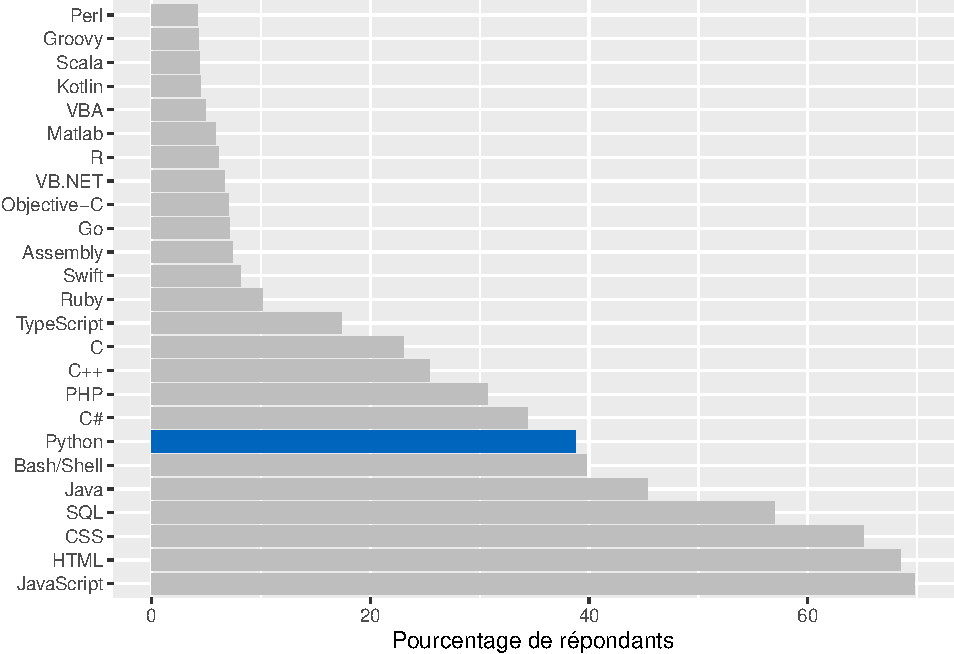
\includegraphics{_main_files/figure-latex/intro-stack-langages-1} 

}

\caption{Langages de programmation, de scripting et de balisage.}\label{fig:intro-stack-langages}
\end{figure}

\section{Versions}\label{versions}

Ces notes de cours visent à fournir une introduction à Python, dans sa
version 3.x. En ce sens, les exemples fournis corresponderont à cette
version, non pas aux précédentes.

Comparativement à la version 2.7, la version 3.0 a apporté des
modofications profondes. Il faut noter que Python 2.7 prendra
``\href{https://pythonclock.org/}{sa retraite}'' le premier janvier
2020. Passée cette date, le support ne sera plus assuré.

\section{Espace de travail}\label{espace-de-travail}

Il existe de nombreux environnements dans lesquels programmer en Python.
Nous allons en présenter succinctement quelques uns.

Il est supposé ici que vous vous avez installé
\href{https://www.anaconda.com/}{Anaconda} sur votre poste. Anaconda est
une distribution gratuite et open source des langages de programmation
Python et R pour les applications en \emph{data science} et
apprentissage automatique. Par ailleurs, lorsqu'il est fait mention du
terminal dans les notes, il est supposé que le système d'exploitation de
votre machine est soit Linux, soit Mac OS.

\subsection{Python dans un terminal}\label{python-dans-un-terminal}

Il est possible d'appeler Python depuis un terminal, en exécutant la
commande suivante (sous Windows : dans le menu démarrer, lancer le
logiciel ``Python 3.6'') :

\begin{lstlisting}
> python
\end{lstlisting}

Ce qui donne le rendu visible sur la
Figure~\ref{fig:intro-python-terminal} :

\begin{figure}[H]

{\centering 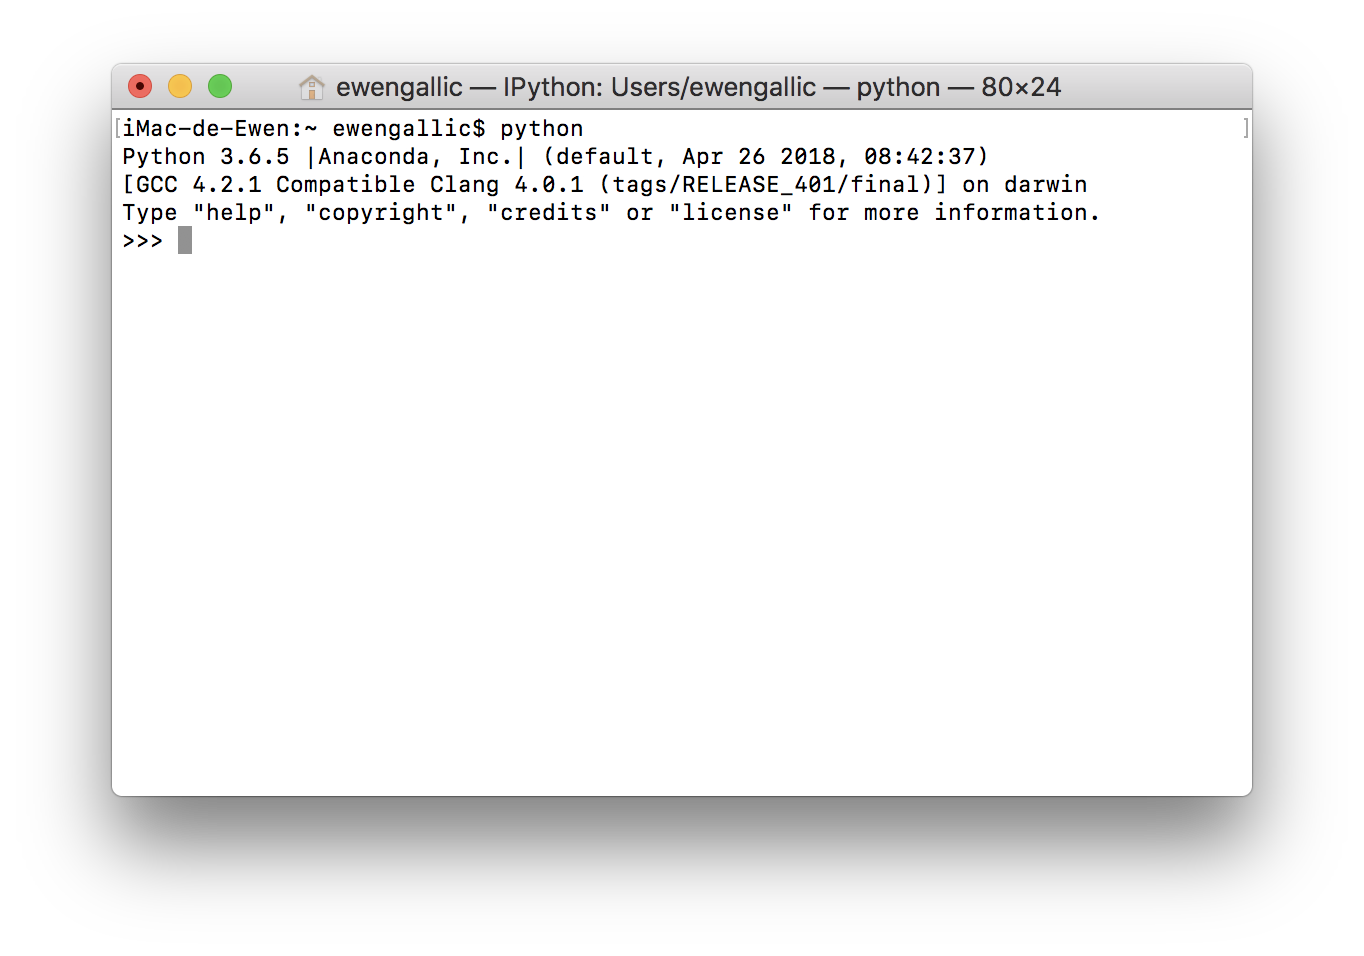
\includegraphics[width=0.7\linewidth]{figs/python_terminal} 

}

\caption{Python dans un terminal.}\label{fig:intro-python-terminal}
\end{figure}

On note la présence des caractères
\texttt{\textgreater{}\textgreater{}\textgreater{}} (\emph{prompt}), qui
invitent l'utilisateur à inscrie une commande. Les expressions sont
évaluées une fois qu'elle sont soumises (à l'aide de la touche
\texttt{ENTREE}) et le résultat est donné, lorsqu'il n'y a pas d'erreur
dans le code.

Par exemple, lorsque l'on évalue \texttt{2+1} :

\begin{lstlisting}
> >>> 2+1
+ 3
+ >>>
\end{lstlisting}

On note la présence du \emph{prompt} à la fin, indiquant que Python est
prêt à recevoir de nouvelles instructions.

\subsection{IPython}\label{ipython}

Il existe un environnement un peu plus chaleureux que Python dans le
terminal : IPython. Il s'agit également d'un terminal interactif, mais
avec davantages de fonctionnalités, notamment la coloration syntaxique
ou l'auto-complétion (en utilisant la touche de tabulation).

Pour lancer IPython, on peut ouvrir un terminal et taper (puis valider)
:

\begin{lstlisting}
> ipython
\end{lstlisting}

On peut également lancer IPython depuis la fenêtre d'accueil d'Anaconda,
en cliquant sur le bouton \texttt{Launch} de l'application
\texttt{qtconsole}, visible sur la
Figure~\ref{fig:intro-anaconda-navigator}.

\begin{figure}[H]

{\centering 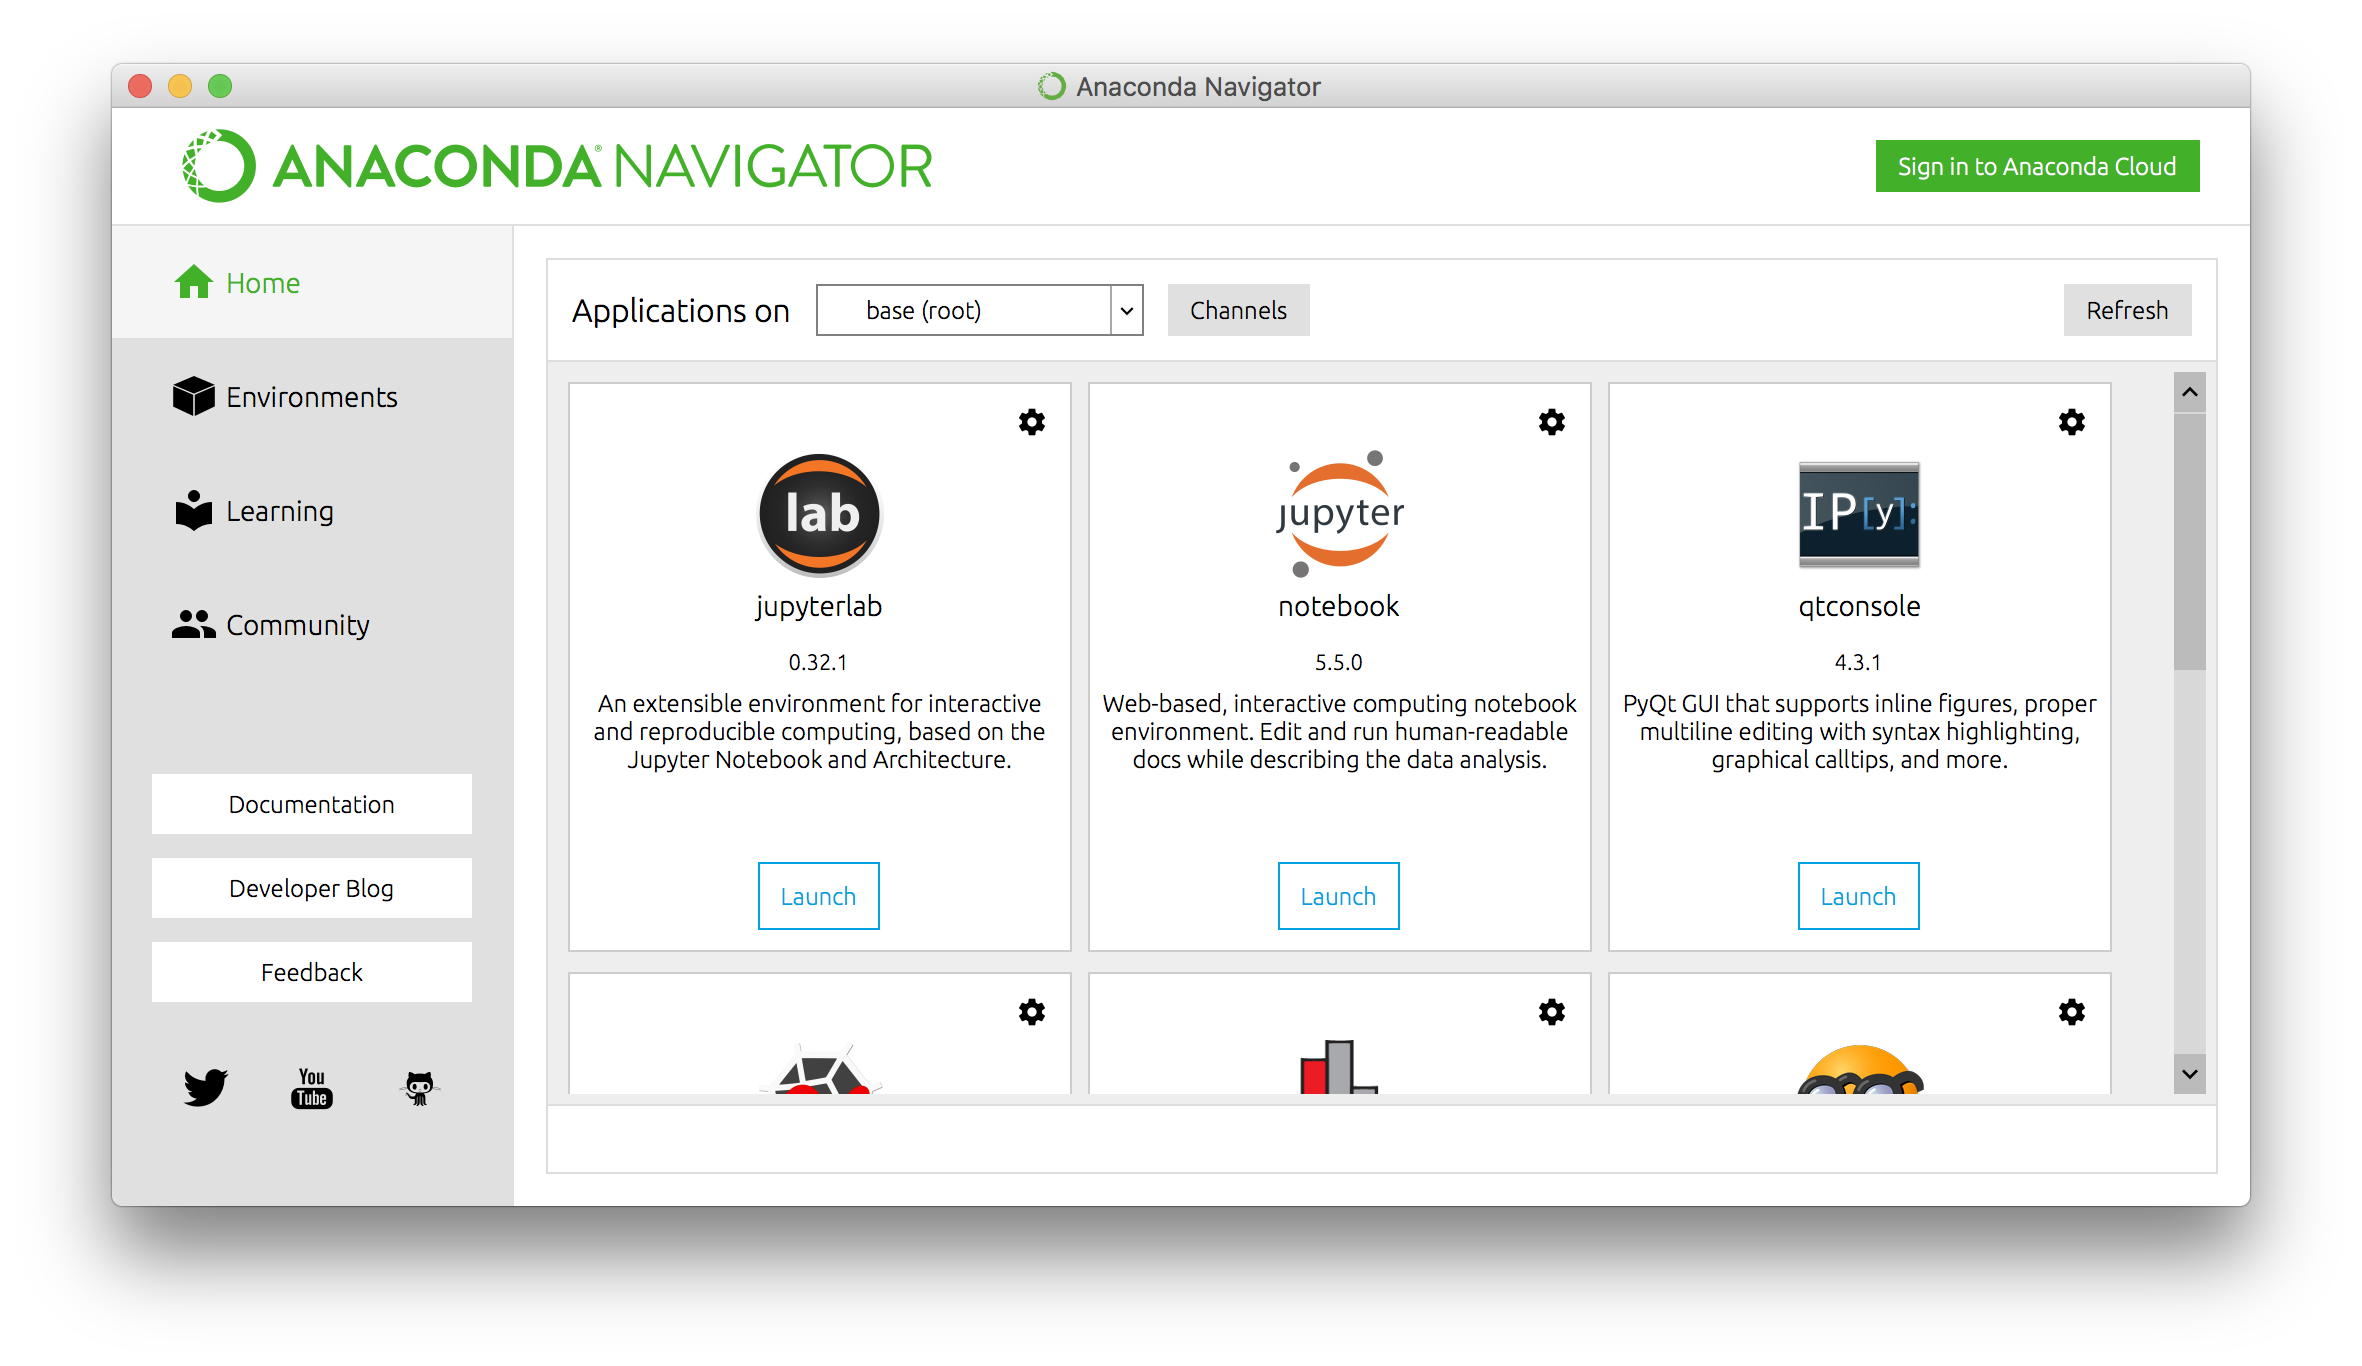
\includegraphics[width=1\linewidth]{figs/anaconda_navigator} 

}

\caption{Fenêtre d'accueil d'Anaconda.}\label{fig:intro-anaconda-navigator}
\end{figure}

La console IPython, une fois lancée, ressemble à ceci :

\begin{figure}[H]

{\centering 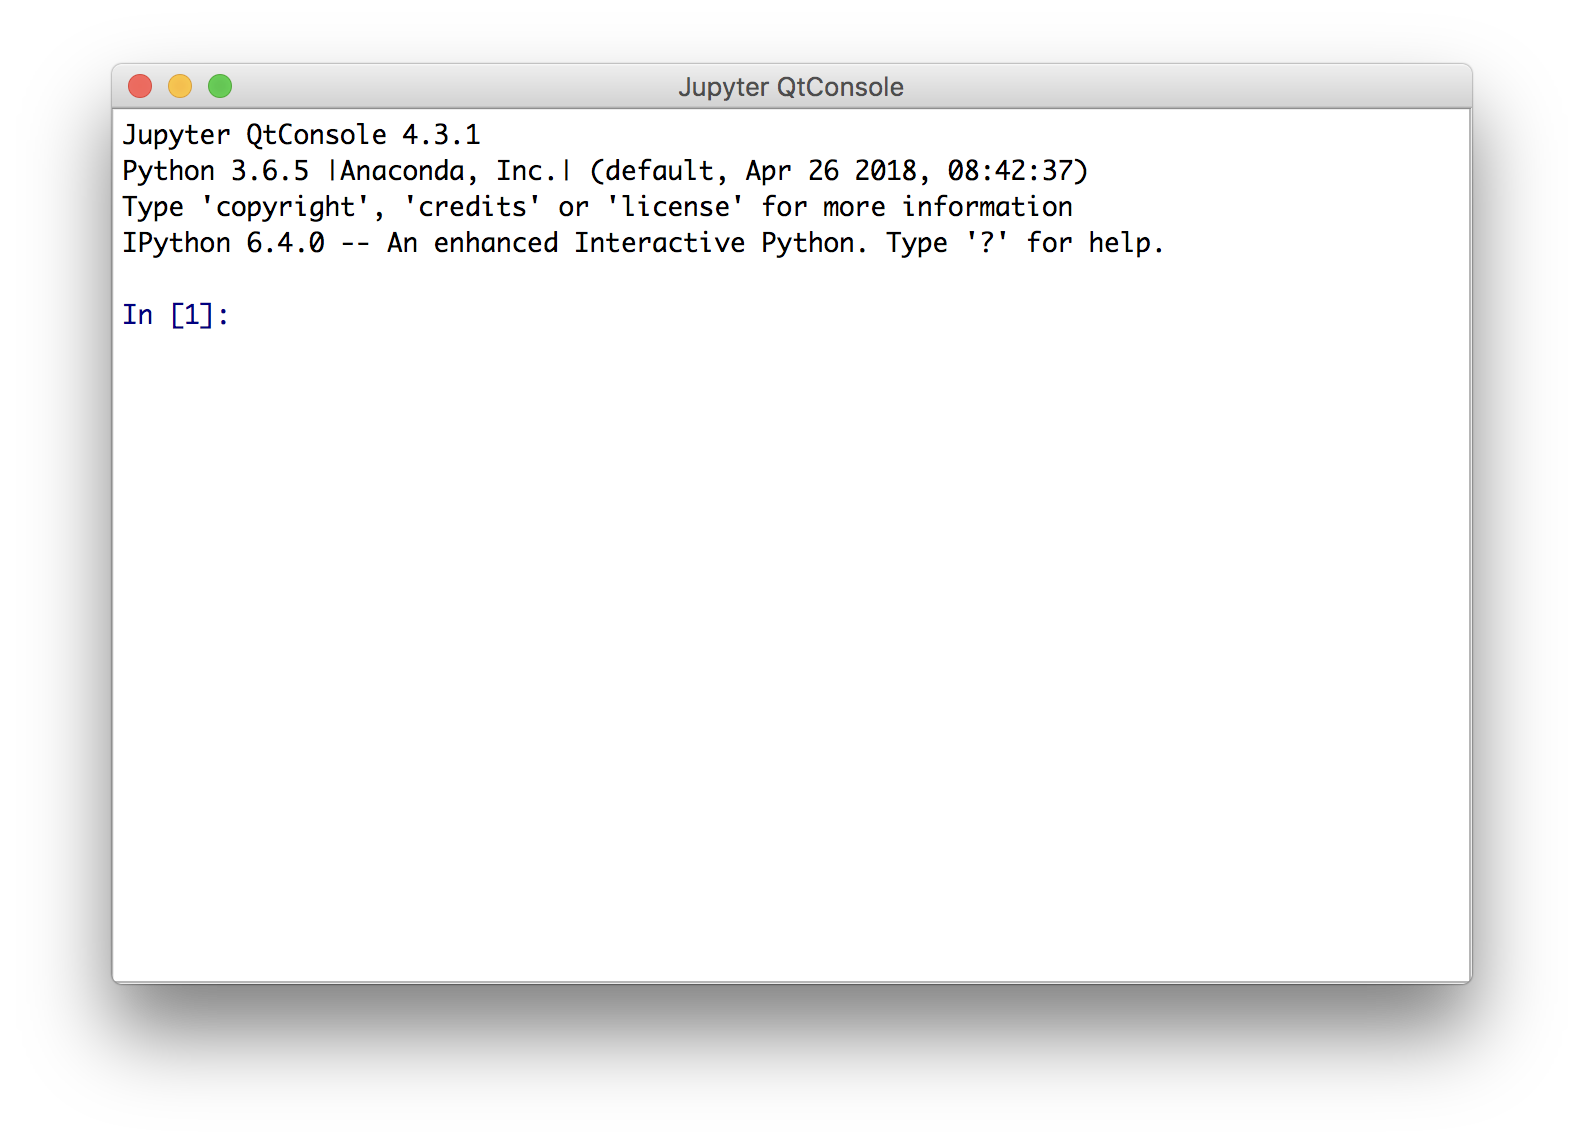
\includegraphics[width=0.7\linewidth]{figs/ipython} 

}

\caption{Console IPython.}\label{fig:unnamed-chunk-5}
\end{figure}

Soumettons une instruction simple pour évaluation à Python :

\begin{Shaded}
\begin{Highlighting}[]
\OperatorTok{>} \BuiltInTok{print}\NormalTok{(}\StringTok{"Hello World"}\NormalTok{)}
\end{Highlighting}
\end{Shaded}

Le résultat donne :

\begin{lstlisting}
> In [1]: print("Hello World")
+ Hello World
+ 
+ In [2]:
\end{lstlisting}

Plusieurs choses sont à noter. Premièrement, on note qu'à la fin de
l'exécution de l'instruction, IPython nous indique qu'il est prêt à
recevoir de nouvelles instruction, par la présence du \emph{prompt}
\texttt{In\ {[}2{]}:}. Le numéro entre les crochets désigne le numéro de
l'instruction. On note qu'il est passé de 1 à 2 après l'exécution.
Ensuite, on note que le résultat de l'appel à la fonction
\texttt{print()}, avec la chaîne de caractères (délimitée par des
guillemets), affiche à l'écran ce qui était contenu entre les
parenthèses.

\subsection{Spyder}\label{spyder}

Tandis que lorsqu'on utilise Python via un terminal, il est préférable
d'avoir un éditeur de texte ouvert à côté (pour pouvoir sauvegarder les
instructions), comme, par exemple,
\href{https://www.sublimetext.com/}{Sublime Text} sous Linux ou Mac OS,
ou \href{https://notepad-plus-plus.org/}{notepad++} sous Windows.

Une autre alternative consiste à utiliser un environnement de
développement (IDE, pour \emph{Integrated development environment})
unique proposant notamment, à la fois un éditeur et une console. C'est
ce que propose \href{https://www.spyder-ide.org/}{Spyder}, avec en outre
de nombreuses fonctionnalités supplémentaires, comme la gestion de
projet, un explorateur de fichier, un historique des commandes, un
débugger, etc.

Pour lancer Spyder, on peut passer par un terminal, en évaluant tout
simplement \texttt{Spyder} (ou en lançant le logiciel depuis le menu
démarrer sous Windows). Il est également possible de lancer Spyder
depuis Anaconda.

L'environnement de développement, comme visible sur la
Figure~\ref{fig:intro-spyder}, se décompose en plusieurs fenêtres :

\begin{itemize}
\tightlist
\item
  à gauche : l'éditeur de script ;
\item
  en haut à droite : une fenêtre permettant d'afficher l'aide de Python,
  l'arborescence du système ou encore les variables créées ;
\item
  en bas à droite : une ou plusieurs consoles.
\end{itemize}

\begin{figure}[H]

{\centering 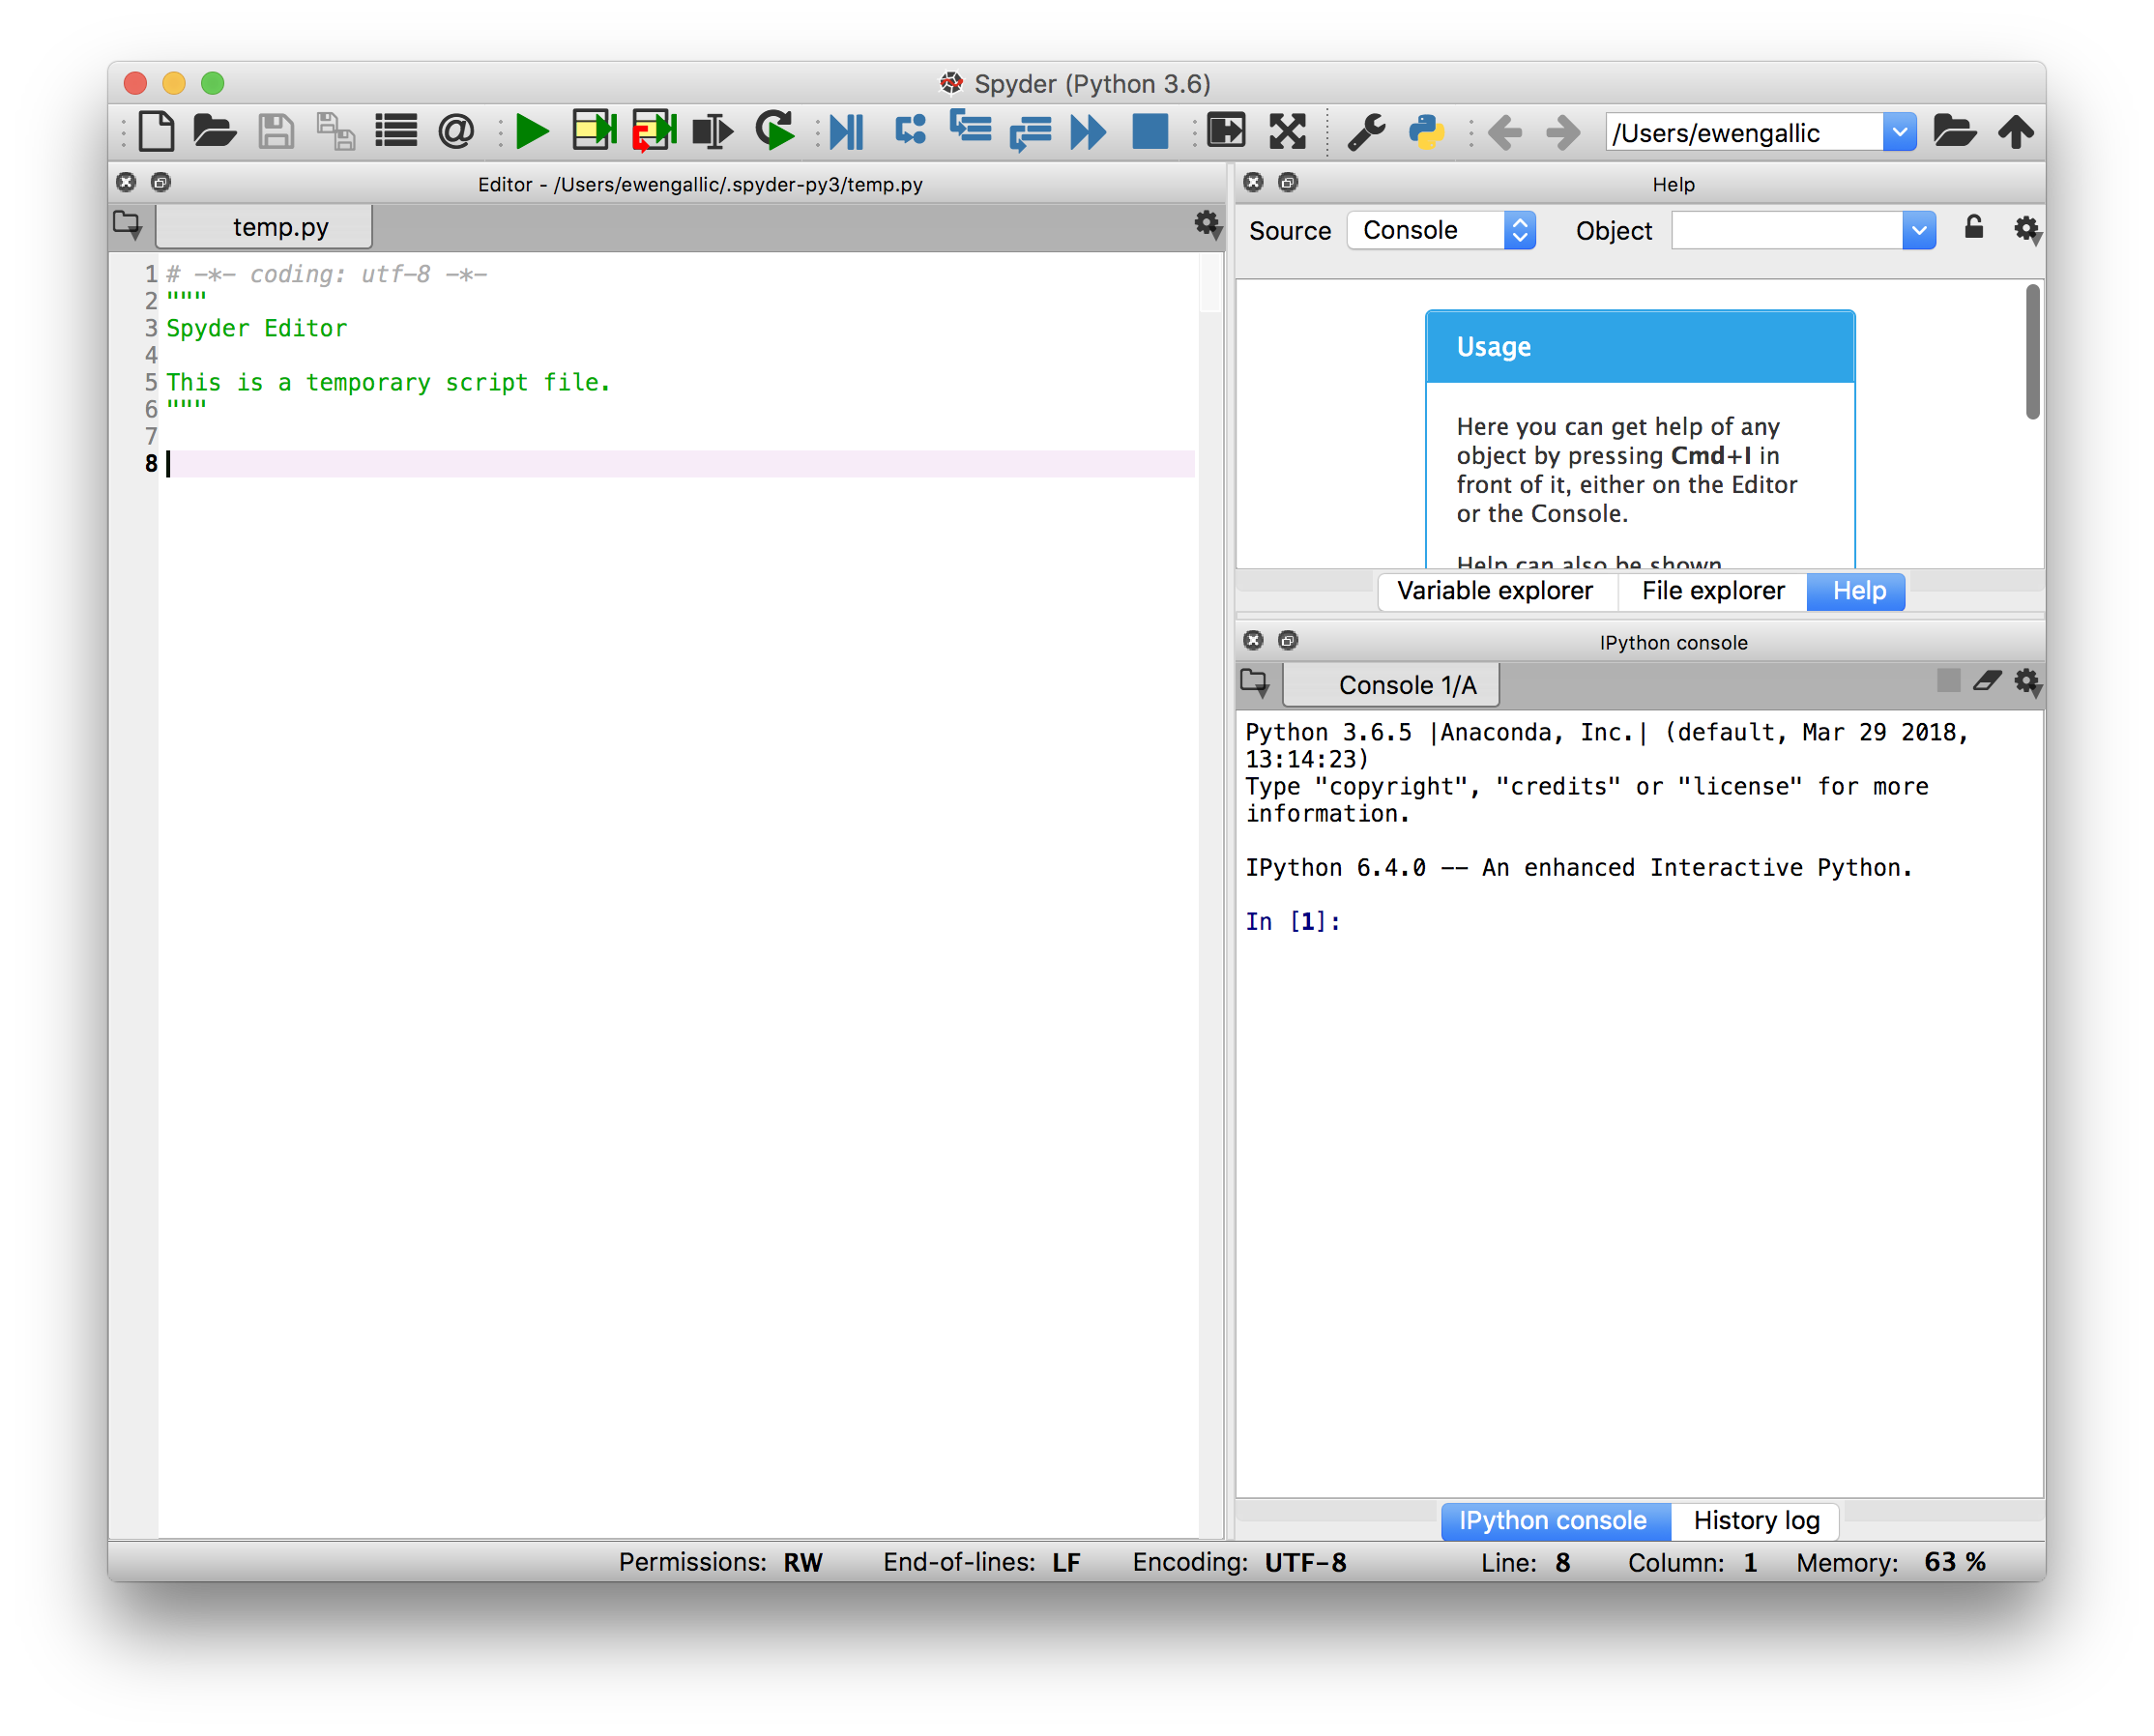
\includegraphics[width=1\linewidth]{figs/spyder} 

}

\caption{Spyder.}\label{fig:intro-spyder}
\end{figure}

\subsection{Jupyter}\label{jupyter}

Il existe une interface graphique par navigateur d'IPython, appelée
\href{http://jupyter.org/}{Jupyter Notebook}. Il s'agit d'une
application en open-source permettant de créer et partager des documents
qui contiennent du code, des équations, des représentations graphiques
et du texte. Il est possible de faire figurer et exécuter des codes de
langages différents dans les notebook Jupyter.

Pour lancer Jupyter, on peut passer par Anaconda. Après avoir cliqué sur
le bouton \texttt{Launch}, de Jupyter Notebook, le navigateur web se
lance et propose une arborescence, comme montré sur la
Figure~\ref{fig:intro-jupyter}. Sans que l'on s'en rendiez compte, un
serveur local web a été lancé ainsi qu'un processus Python (un
\emph{kernel}).

Si le navigateur en se lance pas automatiquement, on peut accéder à la
page qui aurait dû s'afficher, en se rendant à l'adresse suivante :
\url{http://localhost:8890/tree}?.

\begin{figure}[H]

{\centering 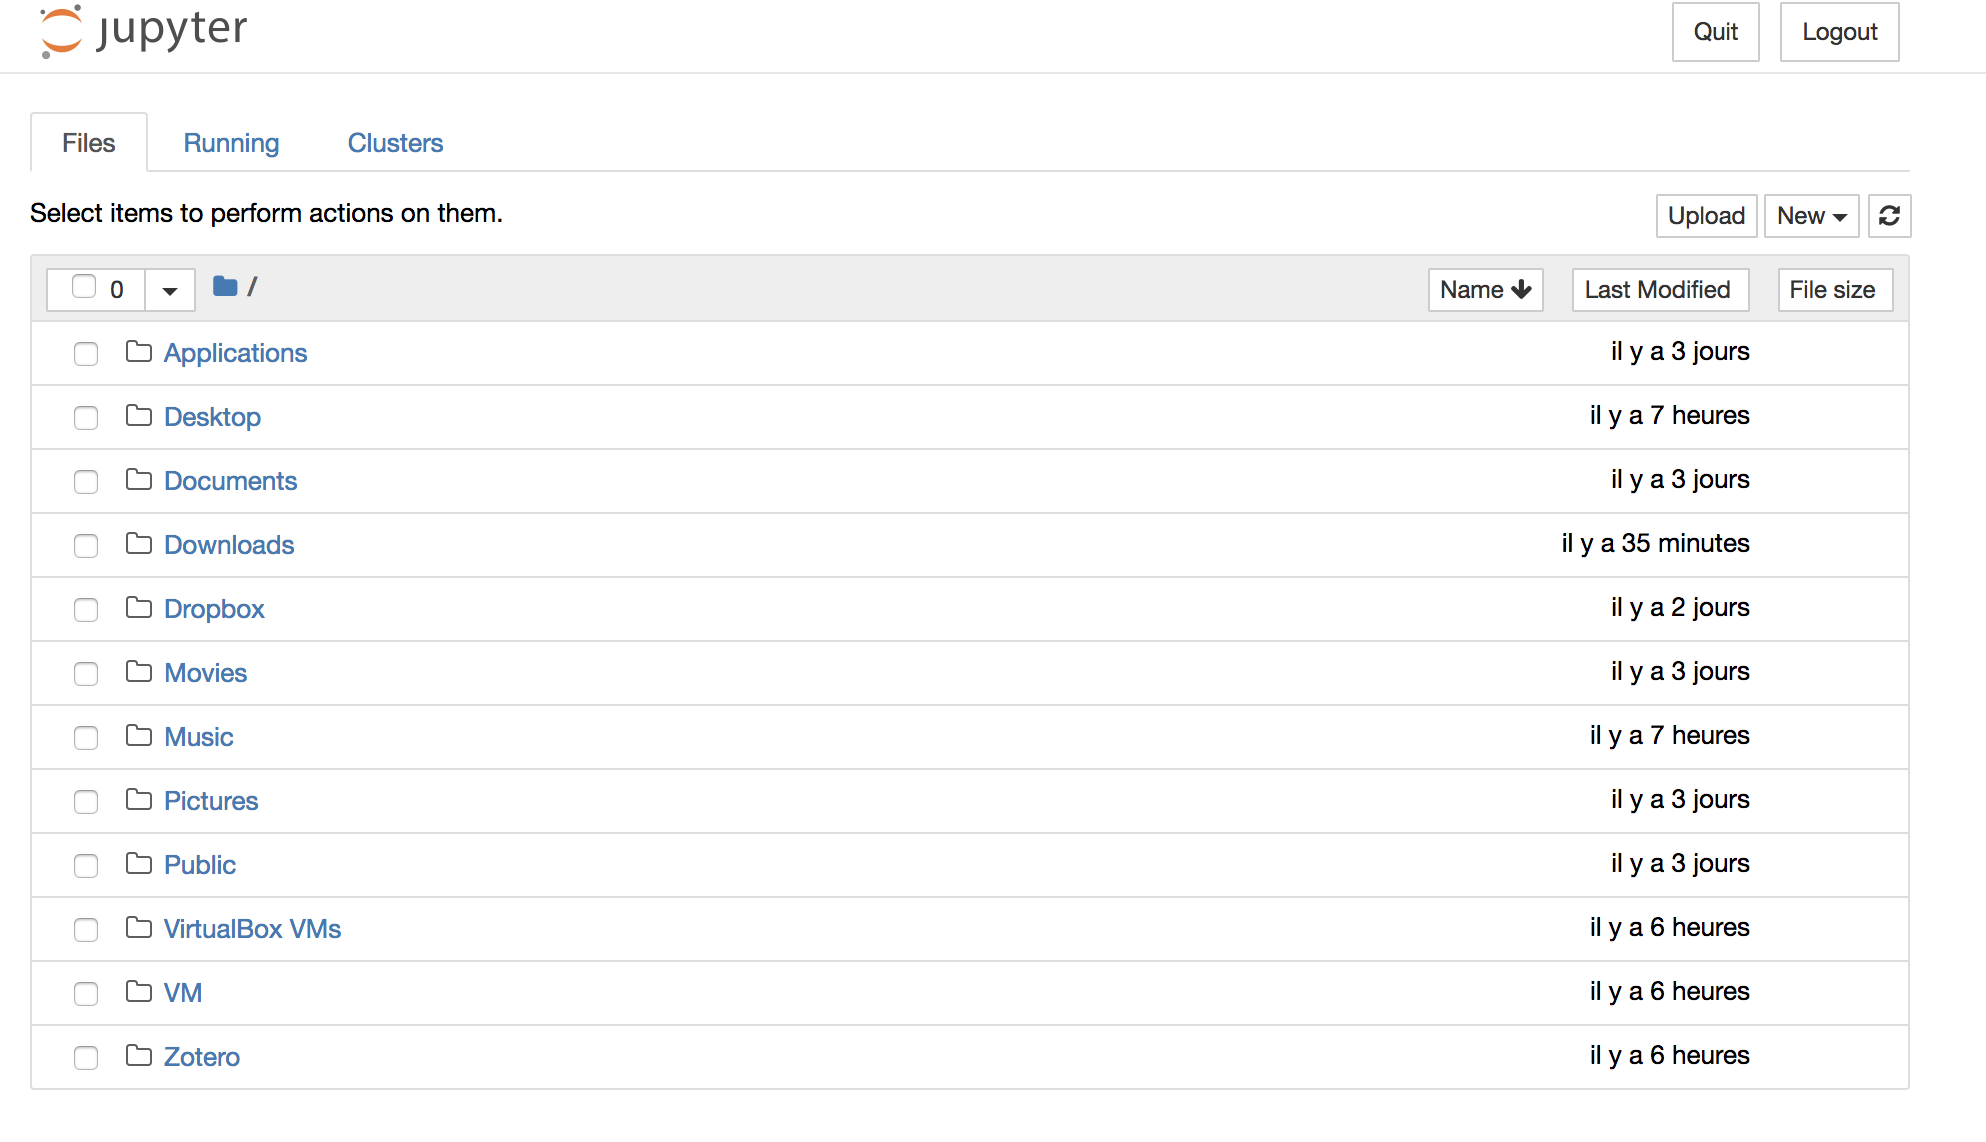
\includegraphics[width=1\linewidth]{figs/jupyter} 

}

\caption{Jupyter.}\label{fig:intro-jupyter}
\end{figure}

Pour aborder les principales fonctions de Jupyter, nous allons créer un
dossier \texttt{jupyter} dans un répertoire de notre choix. Une fois ce
dossier créé, y naviguer à travers l'arborescence de Jupyter, dans le
navigateur web.

Une fois dans le dossier, créer un nouveau Notebook \texttt{Python\ 3}
(en cliquant sur le bouton \texttt{New} en haut à gauche de la fenêtre,
puis sur Python 3`).

Un notebook intitulé \texttt{Untitled} vient d'être créé, la page
affiche un document vide, comme visible sur la
Figure~\ref{fig:intro-jupyter-notebook}.

\begin{figure}[H]

{\centering 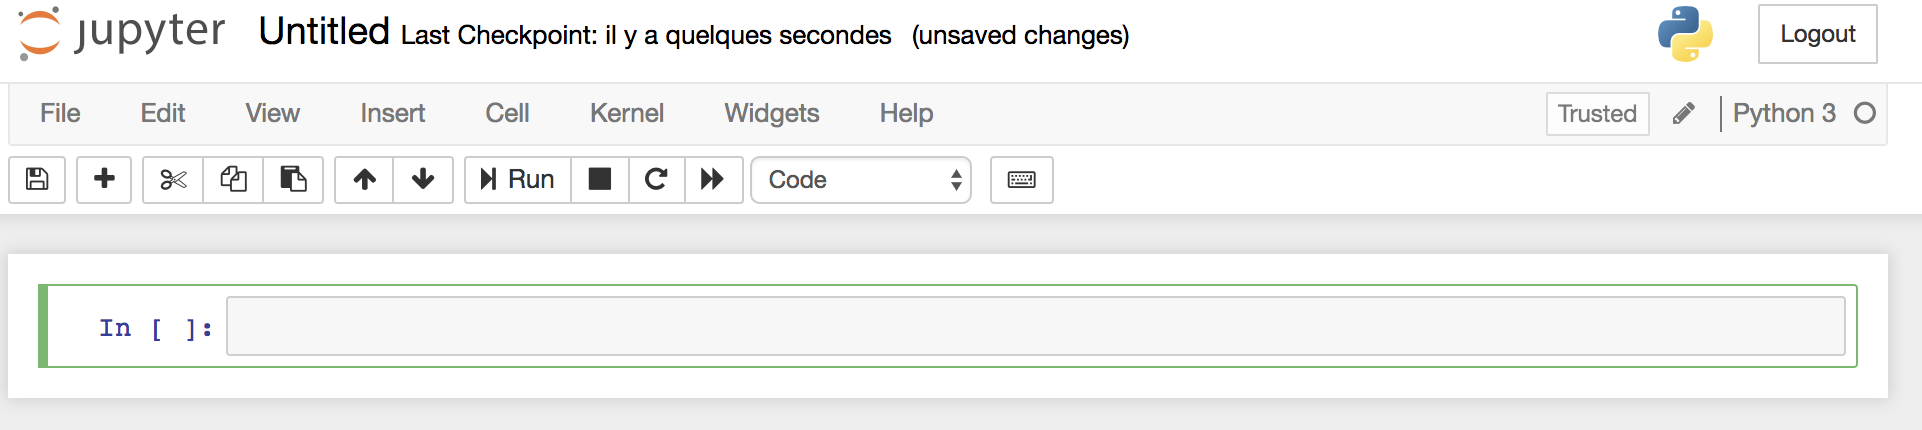
\includegraphics[width=1\linewidth]{figs/jupyter_notebook} 

}

\caption{Un notebook vide.}\label{fig:intro-jupyter-notebook}
\end{figure}

Si on regarde dans notre explorateur de fichier, dans le dossier
\texttt{jupyter} fraîchement créé, un nouveau fichier est apparu :
\texttt{Untitled.ipynb}.

\subsubsection{Évaluation d'une
instruction}\label{evaluation-dune-instruction}

Retournons dans le navigateur web, sur la page affichant notre
\emph{notebook}.

En dessous de la barre des menus, on note la présence d'une zone
encadrée, \textbf{une cellule}, commençant, à l'instar de ce que l'on
voyait dans la console sur IPython, par \texttt{IN\ {[}{]}:}. À droite,
la zone grisée nous invite à soumettre des instructions en Python.

Inscrivons :

\begin{Shaded}
\begin{Highlighting}[]
\OperatorTok{>} \DecValTok{2}\OperatorTok{+}\DecValTok{1}
\end{Highlighting}
\end{Shaded}

Pour soumettre l'instruction à évaluation, il existe plusieurs manières
(il s'assurer d'avoir cliqué à l'intérieur de la cellule) :

\begin{itemize}
\tightlist
\item
  dans la barre des menus : \texttt{Cell\ \textgreater{}\ Run\ Cells} ;
\item
  dans la barre des raccourcis : bouton \texttt{Run} ;
\item
  avec le clavier : maintenir la touche \texttt{CTRL}et presser sur
  \texttt{Entree}.
\end{itemize}

\begin{figure}[H]

{\centering 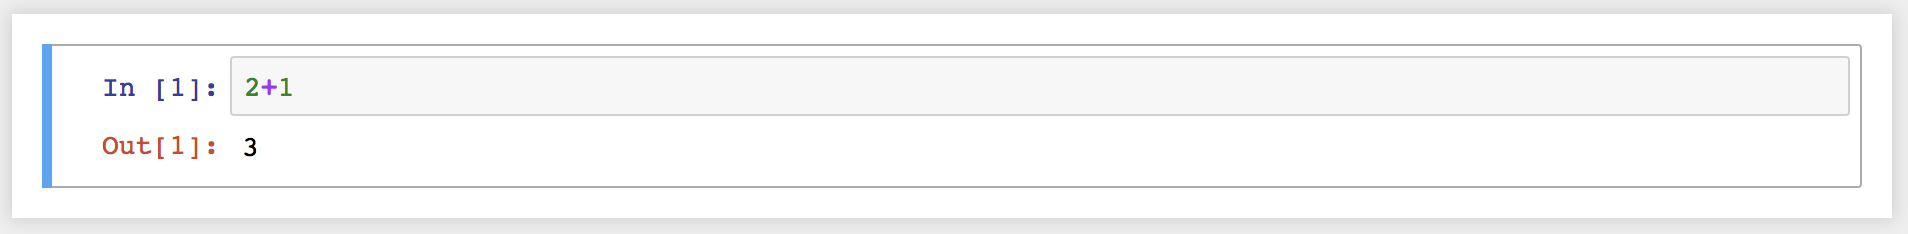
\includegraphics[width=1\linewidth]{figs/jupyter_notebook_2} 

}

\caption{Cellule évaluée.}\label{fig:unnamed-chunk-9}
\end{figure}

\subsubsection{Cellules de texte}\label{cellules-de-texte}

Un des intérêts des \emph{notebooks} est qu'il est possible d'ajouter
des cellules de texte.

Ajoutons une cellule en-dessous de la première. Pour ce faire, on peut
procéder soit :

\begin{itemize}
\tightlist
\item
  par la barre de menu :
  \texttt{Insert\ \textgreater{}\ Insert\ Cell\ Below} (pour insérer une
  cellule en-dessous ; si on désire une insertion au-dessus, il suffit
  de choisir \texttt{Insert\ Cell\ Above}) ;
\item
  en cliquant dans le cadre de la cellule à partir de laquelle on désire
  faire un ajout (n'importe où, sauf dans la zone grisée de code, de
  manière à passer en mode \texttt{commande}), puis en appuyant sur la
  touche \texttt{B} du clavier (\texttt{A} pour une insertion
  au-dessus).
\end{itemize}

La nouvelle cellule appelle à nouveau à inscrire une instruction en
Python. Pour indiquer que le contenu doit être interprété comme du
texte, il est nécessaire de le préciser. Encore une fois, plusieurs
méthodes permettent de le faire :

\begin{itemize}
\tightlist
\item
  par la barre de menu :
  \texttt{Cell\ \textgreater{}\ Cell\ Type\ \textgreater{}\ Markdown} ;
\item
  par la barre des raccourcis : dans le menu déroulant où est inscrit
  \texttt{Code}, en sélectionnant \texttt{Markdown} ;
\item
  en mode commande (après avoir cliqué à l'intérieur du cadre de la
  cellule, mais pas dans la zone de code), en appuyant sur la touche
  \texttt{M} du clavier.
\end{itemize}

La cellule est alors prête à recevoir du texte, rédigé en markdown. Pour
plus d'informations sur la rédaction en Markdown, se référer à cette
\href{https://github.com/adam-p/markdown-here/wiki/Markdown-Cheatsheet}{antisèche}
par exemple.

Entrons quelques lignes de texte pour voir très rapidement le
fonctionnement des cellules rédigées en Markdown.

\begin{lstlisting}
> # Un titre de niveau 1
+ 
+ Je vais écrire *du texte en italique* et aussi **en gras**.
+ 
+ ## Un titre de niveau 2
+ 
+ Je peux faire des listes :
+ 
+ - avec un item ;
+ - un second ;
+ - et un troisième imbriquant une nouvelle liste :
+     - avec un sous-item,
+     - et un second ;
+ - un quatrième incluant une liste imbriquée numérotée :
+     1. avec un sous-item,
+     1. et un autre.
+ 
+ ## Un autre titre de niveau 2
+ 
+ 
+ Je peux même faire figurer des équation $\LaTeX$.
+ Comme par exemple $X \sim \mathcal{N}(0,1)$.
+ 
+ Pour en savoir plus sur $\LaTeX$, on peut se référer à cette :
+   [page Wikipédia](https://en.wikibooks.org/wiki/LaTeX/Mathematics).
\end{lstlisting}

Ce qui donne, dans Jupyter :

\begin{figure}[h]

{\centering 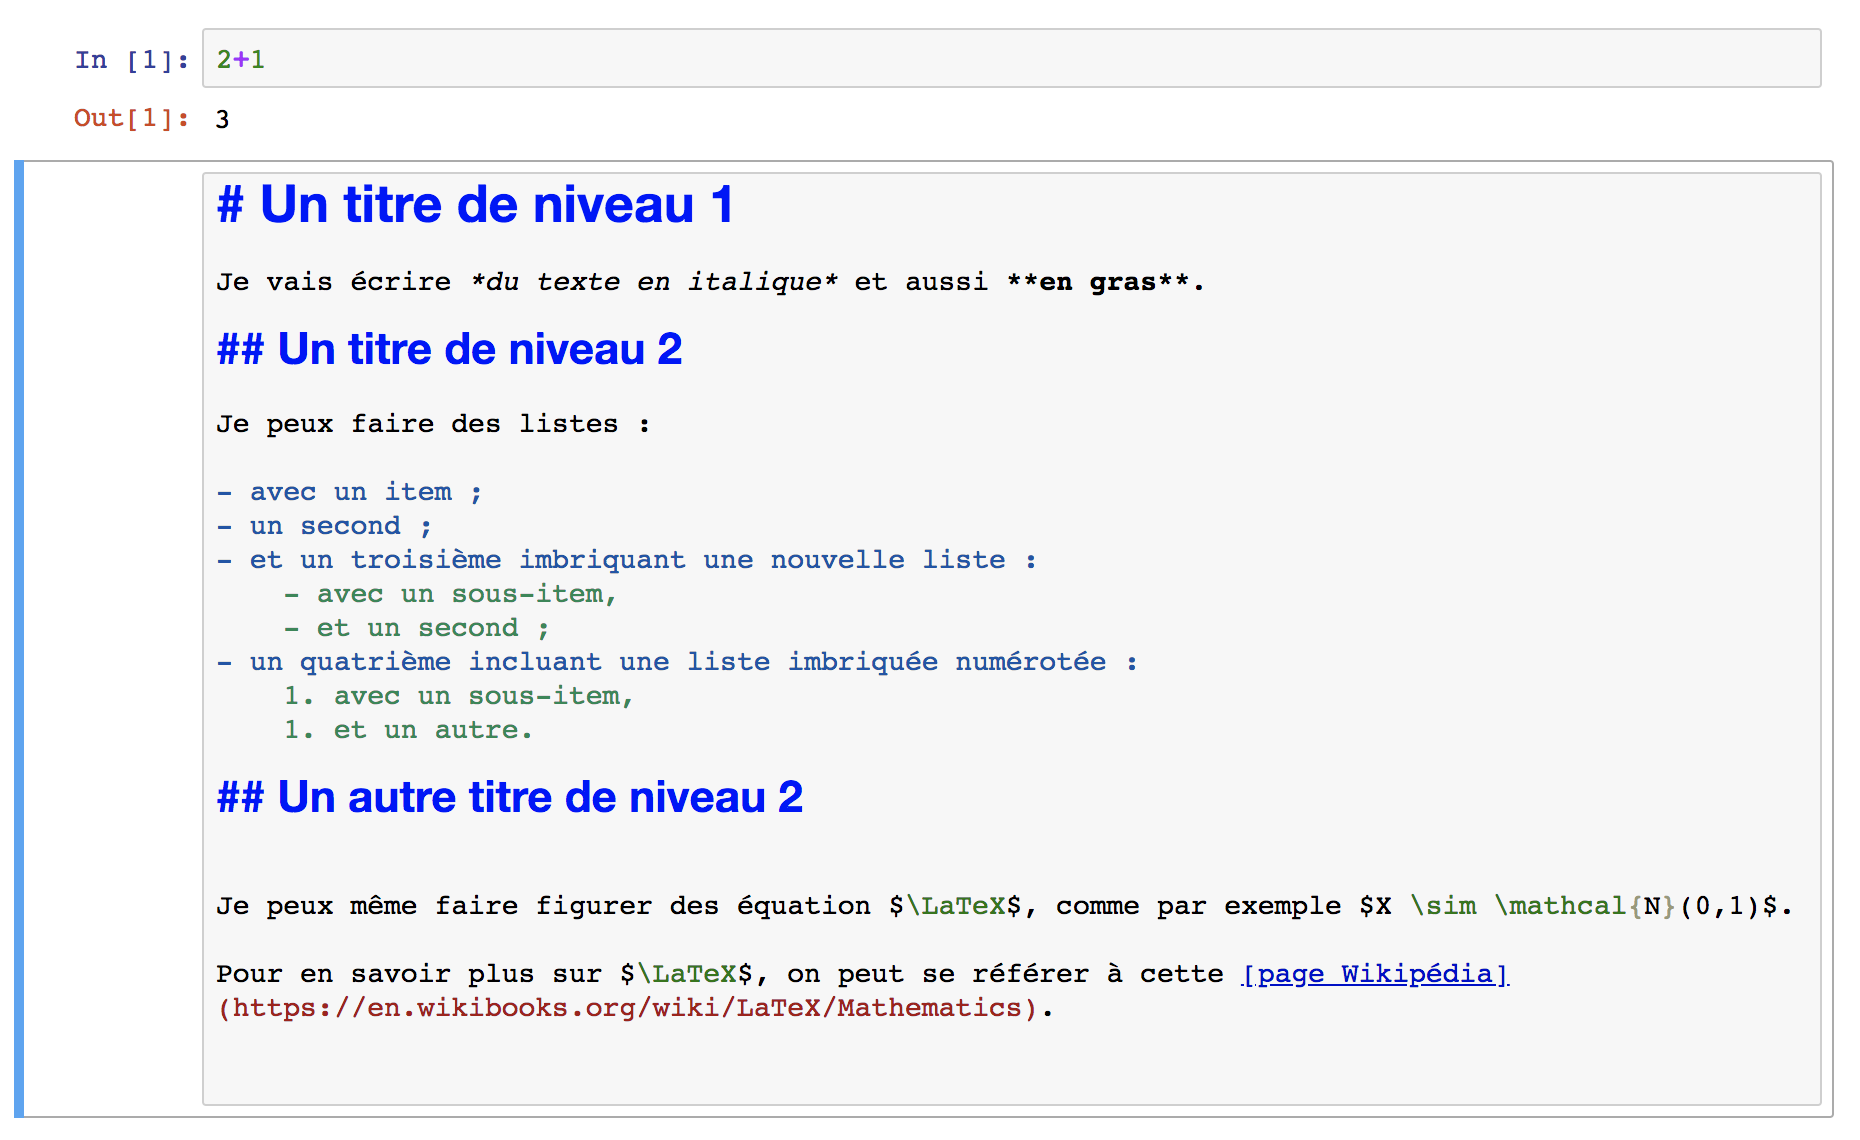
\includegraphics[width=1\linewidth]{figs/jupyter_notebook_3} 

}

\caption{Cellule textuelle non évaluée.}\label{fig:unnamed-chunk-11}
\end{figure}

Reste alors à l'évaluer, comme s'il s'agissait d'une cellule contenant
une instruction Python, pour basculer vers un affichage Markdown
(\texttt{CTRL} et \texttt{ENTREE}).

Pour \textbf{éditer le texte} une fois que l'on a basculé en markdown,
un simple double-clic dans la zone de texte de la cellule fait
l'affaire.

Pour \textbf{changer le type de la cellule pour qu'elle devienne du
code} :

\begin{itemize}
\tightlist
\item
  par la barre de menu :
  \texttt{Cell\ \textgreater{}\ Cell\ Type\ \textgreater{}\ Code} ;
\item
  par la barre des raccourcis : dans le menu déroulant où est inscrit
  \texttt{Code}, en sélectionnant \texttt{Code} ;
\item
  en mode commande, appuyer sur la touche du clavier \texttt{Y}.
\end{itemize}

\subsubsection{Suppression d'une
cellule}\label{suppression-dune-cellule}

Pour supprimer une cellule :

\begin{itemize}
\tightlist
\item
  par la barre de menu : \texttt{Edit\ \textgreater{}\ Delete\ Cells} ;
\item
  par la barre des raccourcis : icône en forme de ciseaux ;
\item
  en mode commande, appuyer deux fois sur la touche du clavier
  \texttt{D}.
\end{itemize}

\section{Les variables}\label{les-variables}

\subsection{Assignation et
suppression}\label{assignation-et-suppression}

Lorsque nous avons évalué les instructions \texttt{2+1} précédemment, le
résultat s'est affiché dans la console, mais il n'a pas été enregistré.
Dans de nombreux cas, il est utile de conserver le contenu du résultat
dans un objet, pour pouvoir le réutiliser par la suite. Pour ce faire,
on utilise des \emph{variables}. Pour créer une variable, on utilise le
signe d'égalité (\texttt{=}), que l'on fait suivre par ce que l'on veut
sauvegarder (du texte, un nombre, plusieurs nombres, etc.) et précéder
par le nom que l'on utilisera pour désigner cette variable.

Par exemple, si on souhaite stocker le résultat du calcul \texttt{2+1}
dans une variable que l'on nommera \texttt{x}, il faudra écrire :

\begin{Shaded}
\begin{Highlighting}[]
\OperatorTok{>}\NormalTok{ x }\OperatorTok{=} \DecValTok{2}\OperatorTok{+}\DecValTok{1}
\end{Highlighting}
\end{Shaded}

Pour afficher la valeur de notre variable \texttt{x}, on fait appel à la
fonction \texttt{print()} :

\begin{Shaded}
\begin{Highlighting}[]
\OperatorTok{>} \BuiltInTok{print}\NormalTok{(x)}
\end{Highlighting}
\end{Shaded}

\begin{lstlisting}
## 3
\end{lstlisting}

Pour changer la valeur de la variable, il suffit de faire une nouvelle
assignation :

\begin{Shaded}
\begin{Highlighting}[]
\OperatorTok{>}\NormalTok{ x }\OperatorTok{=} \DecValTok{4}
\OperatorTok{+} \BuiltInTok{print}\NormalTok{(x)}
\end{Highlighting}
\end{Shaded}

\begin{lstlisting}
## 4
\end{lstlisting}

Il est également possible de donner plus d'un nom à un même contenu (on
réalise une copie de \texttt{x}) :

\begin{Shaded}
\begin{Highlighting}[]
\OperatorTok{>}\NormalTok{ x }\OperatorTok{=} \DecValTok{4}\OperatorTok{;}
\OperatorTok{+}\NormalTok{ y }\OperatorTok{=}\NormalTok{ x}\OperatorTok{;}
\OperatorTok{+} \BuiltInTok{print}\NormalTok{(y)}
\end{Highlighting}
\end{Shaded}

\begin{lstlisting}
## 4
\end{lstlisting}

Si on modifie la copie, l'original ne sera pas affecté :

\begin{Shaded}
\begin{Highlighting}[]
\OperatorTok{>}\NormalTok{ y }\OperatorTok{=} \DecValTok{0}
\OperatorTok{+} \BuiltInTok{print}\NormalTok{(y)}
\end{Highlighting}
\end{Shaded}

\begin{lstlisting}
## 0
\end{lstlisting}

\begin{Shaded}
\begin{Highlighting}[]
\OperatorTok{>} \BuiltInTok{print}\NormalTok{(x)}
\end{Highlighting}
\end{Shaded}

\begin{lstlisting}
## 4
\end{lstlisting}

Pour \textbf{supprimer} une variable, on utilise l'instruction
\texttt{del} :

\begin{Shaded}
\begin{Highlighting}[]
\OperatorTok{>} \KeywordTok{del}\NormalTok{ y}
\end{Highlighting}
\end{Shaded}

L'affichage du contenu de \texttt{y} renvoit une erreur :

\begin{Shaded}
\begin{Highlighting}[]
\OperatorTok{>} \BuiltInTok{print}\NormalTok{(y)}
\end{Highlighting}
\end{Shaded}

\begin{lstlisting}
## NameError: name 'y' is not defined
## 
## Detailed traceback: 
##   File "<string>", line 1, in <module>
\end{lstlisting}

Mais on note que la variable \texttt{x} n'a pas été supprimée :

\begin{Shaded}
\begin{Highlighting}[]
\OperatorTok{>} \BuiltInTok{print}\NormalTok{(x)}
\end{Highlighting}
\end{Shaded}

\begin{lstlisting}
## 4
\end{lstlisting}

\subsection{Conventions de nommage}\label{conventions-de-nommage}

Le nom d'une variable peut être composé de caractères alphanumériques
ainsi que du trait de soulignement (\texttt{\_}) (il n'y a pas de limite
sur la longueur du nom). Il est proscrit de faire commencer le nom de la
variable par un nombre. Il est également interdit de faire figurer une
espace dans le nom d'une variable.

Pour accroitre la lisibilité du nom des variables, plusieurs méthodes
existes. Nous adopterons la suivante :

\begin{itemize}
\tightlist
\item
  toutes les lettres en minuscule ;
\item
  la séparation des termes par un trait de soulignement.
\end{itemize}

Exemple, pour une variable contenant la valeur de l'identifiant d'un
utilisateur : \texttt{id\_utilisateur}.

Il faut noter que le nom des variables est \textbf{sensible à la casse}
:

\begin{Shaded}
\begin{Highlighting}[]
\OperatorTok{>}\NormalTok{ x }\OperatorTok{=} \StringTok{"toto"}
\OperatorTok{+} \BuiltInTok{print}\NormalTok{(x)}
\end{Highlighting}
\end{Shaded}

\begin{lstlisting}
## toto
\end{lstlisting}

\begin{Shaded}
\begin{Highlighting}[]
\OperatorTok{>} \BuiltInTok{print}\NormalTok{(X)}
\end{Highlighting}
\end{Shaded}

\begin{lstlisting}
## NameError: name 'X' is not defined
## 
## Detailed traceback: 
##   File "<string>", line 1, in <module>
\end{lstlisting}

\section{Les commentaires}\label{les-commentaires}

Pour ajouter des commentaires en python, il existe plusieurs façons.

Une des manières de faire est d'utiliser le symbole dièse (\texttt{\#})
pour effectuer un \textbf{commentaire sur une seule ligne}. Tout ce qui
suit le dièse jusqu'à la fin de la ligne ne sera pas évalué par Python.
En revanche, ce qui vient avant le dièse le sera.

\begin{Shaded}
\begin{Highlighting}[]
\OperatorTok{>} \CommentTok{# Un commentaire print("Bonjour")}
\OperatorTok{+} \BuiltInTok{print}\NormalTok{(}\StringTok{"Hello"}\NormalTok{) }\CommentTok{# Un autre commentaire}
\end{Highlighting}
\end{Shaded}

\begin{lstlisting}
## Hello
\end{lstlisting}

L'introduction d'un \textbf{bloc de commentaires} (des commentaires sur
plusieurs lignes) s'effectue quant à elle en entourant ce qui est )
commenter d'un délimiteur : trois guillemets simples ou doubles :

\begin{Shaded}
\begin{Highlighting}[]
\OperatorTok{>} \StringTok{"""}
\StringTok{+ Un commentaire qui commencer sur une ligne}
\StringTok{+ et qui continue sur une autre}
\StringTok{+ et s'arrête à la troisième}
\StringTok{+ """}
\end{Highlighting}
\end{Shaded}

\section{Les modules et les packages}\label{les-modules-et-les-packages}

Certaines fonctions de base en Python sont chargées par défaut.
D'autres, nécessitent de charger un \textbf{module}. Ces modules sont
des fichiers qui contiennent des \textbf{définitions} ainsi que des
\textbf{instructions}.

Lorsque plusieurs modules sont réunis pour offrir un ensemble de
fonctions, on parle alors de \emph{\textbf{package}}.

Parmi les \emph{packages} qui seront utilisés dans ces notes, on peut
citer :

\begin{itemize}
\tightlist
\item
  \href{http://www.numpy.org/}{NumPy}, un \emph{package} fondamental
  pour effectuer des calculs scientifiques ;
\item
  \href{https://pandas.pydata.org/}{pandas}, un \emph{package}
  permettant de manipuler facilement les données et de les analyser ;
\item
  \href{https://matplotlib.org/}{Matplotlib}, un \emph{package}
  permettant de réaliser des graphiques.
\end{itemize}

Pour charger un module (ou un \emph{package}), on utilise la commande
\texttt{import}. Par exemple, pour charger le \emph{package}
\texttt{pandas} :

\begin{Shaded}
\begin{Highlighting}[]
\OperatorTok{>} \ImportTok{import}\NormalTok{ pandas}
\end{Highlighting}
\end{Shaded}

Ce qui permet de faire appel à des fonctions contenues dans le module ou
le \emph{package}. Par exemple, ici, on peut faire appel à la fonction
\texttt{Series()}, contenue dans le \emph{package} \texttt{pandas},
permettant de créer un tableau de données indexées à une dimension :

\begin{Shaded}
\begin{Highlighting}[]
\OperatorTok{>}\NormalTok{ x }\OperatorTok{=}\NormalTok{ pandas.Series([}\DecValTok{1}\NormalTok{, }\DecValTok{5}\NormalTok{, }\DecValTok{4}\NormalTok{])}
\OperatorTok{+} \BuiltInTok{print}\NormalTok{(x)}
\end{Highlighting}
\end{Shaded}

\begin{lstlisting}
## 0    1
## 1    5
## 2    4
## dtype: int64
\end{lstlisting}

Il est possible de donner un alias au module ou au \emph{package} que
l'on importe, en le précisant à l'aide de la syntaxe suivante :

\begin{Shaded}
\begin{Highlighting}[]
\OperatorTok{>} \ImportTok{import}\NormalTok{ module }\ImportTok{as}\NormalTok{ alias}
\end{Highlighting}
\end{Shaded}

Cette pratique est courante pour abréger les noms des modules que l'on
va être amené à utiliser beaucoup. Par exemple, pour \texttt{pandas}, il
est coutume d'écourter le nom en \texttt{pd} :

\begin{Shaded}
\begin{Highlighting}[]
\OperatorTok{>} \ImportTok{import}\NormalTok{ pandas }\ImportTok{as}\NormalTok{ pd}
\OperatorTok{+}\NormalTok{ x }\OperatorTok{=}\NormalTok{ pd.Series([}\DecValTok{1}\NormalTok{, }\DecValTok{5}\NormalTok{, }\DecValTok{4}\NormalTok{])}
\OperatorTok{+} \BuiltInTok{print}\NormalTok{(x)}
\end{Highlighting}
\end{Shaded}

\begin{lstlisting}
## 0    1
## 1    5
## 2    4
## dtype: int64
\end{lstlisting}

On peut également importer une seule fonction d'un module, et lui
attribuer (optionnellement) un alias. Par exemple, avec la fonction
\texttt{pyplot} du \emph{package} \texttt{matplotlib}, il est coutume de
faire comme suit :

\begin{Shaded}
\begin{Highlighting}[]
\OperatorTok{>} \ImportTok{import}\NormalTok{ matplotlib}
\OperatorTok{+} \ImportTok{import}\NormalTok{ matplotlib.pyplot  }\ImportTok{as}\NormalTok{ plt}
\OperatorTok{+} \ImportTok{import}\NormalTok{ numpy  }\ImportTok{as}\NormalTok{ np}
\OperatorTok{+}\NormalTok{ x }\OperatorTok{=}\NormalTok{ np.arange(}\DecValTok{0}\NormalTok{, }\DecValTok{5}\NormalTok{, }\FloatTok{0.1}\NormalTok{)}\OperatorTok{;}
\OperatorTok{+}\NormalTok{ y }\OperatorTok{=}\NormalTok{ np.sin(x)}
\OperatorTok{+}\NormalTok{ plt.plot(x, y)}
\end{Highlighting}
\end{Shaded}

\begin{center}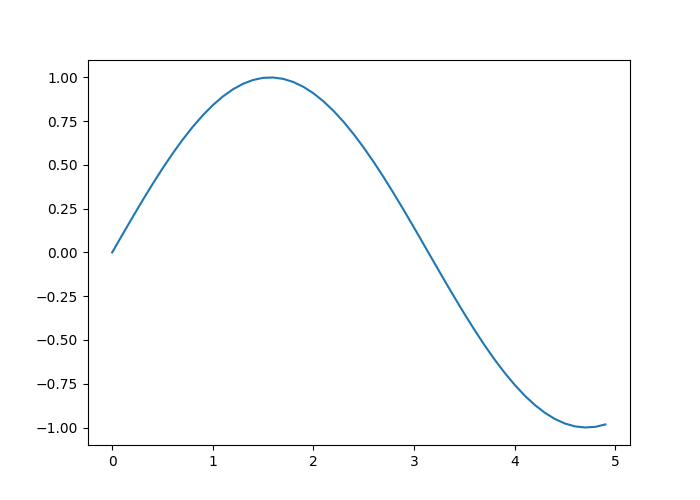
\includegraphics[width=9.03in]{figs/intro_pyplot} \end{center}

\section{L'aide}\label{laide}

Pour conclure cette introduction, il semble important de mentionner la
présence de l'\textbf{aide} et de la \textbf{documentation} en Python.

Pour obtenir des informations sur des fonctions, il est possible de se
référer à la \href{https://docs.python.org/3/}{documentation en ligne}.
Il est également possible d'obtenir de l'aide à l'intérieur de
l'environnement que l'on utilise, en utilisant le point d'interrogation
(\texttt{?}).

Par exemple, lorsque l'on utilise IPython (ce qui, rappelons-le, est le
cas dans Jupyter), on peut accéder à l'aide à travers différentes
syntaxes :

\begin{itemize}
\tightlist
\item
  \texttt{?} : fournit une introduction et un aperçu des fonctionnalités
  offertes en Python (on la quitte avec la touche \texttt{ESC} par
  exemple);
\item
  \texttt{object?} : fournit des détails au sujet de
  \texttt{\textquotesingle{}object\textquotesingle{}} (par exemple
  \texttt{x?} ou encore \texttt{plt.plot?}) ;
\item
  \texttt{object??} : plus de détails à propos de
  \texttt{\textquotesingle{}object\textquotesingle{}} ;
\item
  \texttt{\%quickref} : référence courte sur les syntaxes en Python ;
\item
  \texttt{help()} : accès à l'aide de Python.
\end{itemize}

\emph{Note} : la touche de \textbf{tabulation} du clavier permet non
seulement une \textbf{autocomplétion}, mais aussi une
\textbf{exploration du contenu} d'un objet ou module.

Par ailleurs, lorsqu'il s'agit de trouver de l'aide sur un problème plus
complèxe, le bon réflèxe à adopter est de ne pas hésiter à chercher sur
un moteur de recherche, dans des mailing-lists et bien évidemment sur
les nombreuses questions sur \href{https://stackoverflow.com}{Stack
Overflow}.

\chapter{Types de données}\label{types-de-donnees}

Il existe quelques types de données intégrés dans Python. Nous allons
dans cette partie évoquer les chaînes de caractères, les valeurs
numériques, les bouléens (\texttt{TRUE}/\texttt{FALSE}), la valeur
\texttt{null} et les dates et temps.

\section{Chaînes de caractères}\label{chaines-de-caracteres}

Une chaîne de caractères, ou \emph{string} en anglais, est une
collection de caractères comme des lettres, des nombres, des espaces,
des signes de ponctuation, etc.

Les chaînes de caractères sont repérées à l'aide de guillemets simples,
doubles, ou triples.

Voici un exemple :

\begin{Shaded}
\begin{Highlighting}[]
\OperatorTok{>}\NormalTok{ x }\OperatorTok{=} \StringTok{"Hello World"}
\end{Highlighting}
\end{Shaded}

Pour afficher dans la console le contenu de notre variable \texttt{x}
contenant la chaîne de caractères, on fait appel à la fonction
\texttt{print()} :

\begin{Shaded}
\begin{Highlighting}[]
\OperatorTok{>} \BuiltInTok{print}\NormalTok{(x)}
\end{Highlighting}
\end{Shaded}

\begin{lstlisting}
## Hello World
\end{lstlisting}

Comme indiqué juste avant, des guillemets simples peuvent être utilisés
pour créer une chaîne de caractères :

\begin{Shaded}
\begin{Highlighting}[]
\OperatorTok{>}\NormalTok{ y }\OperatorTok{=} \StringTok{'How are you?'}
\OperatorTok{+} \BuiltInTok{print}\NormalTok{(y)}
\end{Highlighting}
\end{Shaded}

\begin{lstlisting}
## How are you?
\end{lstlisting}

Pour faire figurer des apostrophes dans une chaîne de caractères créée à
l'aide de guillemets simples, il est nécessaire d'utiliser un caracrère
d'échappement : une barre oblique inversée (\texttt{\textbackslash{}}) :

\begin{Shaded}
\begin{Highlighting}[]
\OperatorTok{>}\NormalTok{ z }\OperatorTok{=} \StringTok{'I}\CharTok{\textbackslash{}'}\StringTok{m fine'}
\OperatorTok{+} \BuiltInTok{print}\NormalTok{(z)}
\end{Highlighting}
\end{Shaded}

\begin{lstlisting}
## I'm fine
\end{lstlisting}

On peut noter que si la chaîne de caractères est créée à l'aide de
guillemets doubles, il n'est pas nécessaire d'avoir recours au caractère
d'échappement :

\begin{Shaded}
\begin{Highlighting}[]
\OperatorTok{>}\NormalTok{ z }\OperatorTok{=} \StringTok{"I'm }\CharTok{\textbackslash{}"}\StringTok{fine}\CharTok{\textbackslash{}"}\StringTok{"}
\OperatorTok{+} \BuiltInTok{print}\NormalTok{(z)}
\end{Highlighting}
\end{Shaded}

\begin{lstlisting}
## I'm "fine"
\end{lstlisting}

Pour indiquer un retour à la ligne, on utilise la chaîne
\texttt{\textbackslash{}n} :

\begin{Shaded}
\begin{Highlighting}[]
\OperatorTok{>}\NormalTok{ x }\OperatorTok{=} \StringTok{"Hello, }\CharTok{\textbackslash{}n}\StringTok{World"}
\OperatorTok{+} \BuiltInTok{print}\NormalTok{(x)}
\end{Highlighting}
\end{Shaded}

\begin{lstlisting}
## Hello, 
## World
\end{lstlisting}

Dans le cas de chaînes de caractères sur \textbf{plusieurs lignes}, le
fait d'utiliser des guillemets simples ou doubles renverra une erreur
(\emph{EOL while scanning trial literal}, \emph{i.e.}, détection d'une
erreur de syntaxe, Python s'attendait à quelque chose d'autre à la fin
de la ligne). Pour écrire une chaîne de caractères sur plusieurs lignes,
Python propose d'utiliser trois fois des guillemets (simples ou doubles)
en début et fin de chaîne :

\begin{Shaded}
\begin{Highlighting}[]
\OperatorTok{>}\NormalTok{ x }\OperatorTok{=} \StringTok{"""Hello,}
\StringTok{+ World"""}
\OperatorTok{+} \BuiltInTok{print}\NormalTok{(x)}
\end{Highlighting}
\end{Shaded}

\begin{lstlisting}
## Hello,
## World
\end{lstlisting}

\BeginKnitrBlock{remarque}
Le caractère \texttt{\textbackslash{}} (barre oblique inversée, ou
\emph{backslash}) est le caractère d'échappement. Il permet d'afficher
certains caractères, comme les guillemets dans une chaîne elle-même
définie à l'aide de guillemets, ou bien les caractères de contrôle,
comme la tabulation, le saut de ligne, etc. Voici quelques exemples
courants :

\begin{longtable}[]{@{}cccc@{}}
\toprule
Code & Description & Code & Description\tabularnewline
\midrule
\endhead
\texttt{\textbackslash{}n} & Nouvelle ligne & \texttt{\textbackslash{}r}
& Retour à la ligne\tabularnewline
\texttt{\textbackslash{}t} & Tabulation & \texttt{\textbackslash{}b} &
Retour arrière\tabularnewline
\texttt{\textbackslash{}} & Barre oblique inversée &
\texttt{\textbackslash{}\textquotesingle{}} & Apostrophe\tabularnewline
\texttt{\textbackslash{}"} & Apostrophe double &
\texttt{\textbackslash{}\textasciigrave{}} & Accent grave\tabularnewline
\bottomrule
\end{longtable}
\EndKnitrBlock{remarque}

Pour récupérer la \textbf{longueur d'une chaîne de caractères}, Python
propose la fonction \texttt{len()} :

\begin{Shaded}
\begin{Highlighting}[]
\OperatorTok{>}\NormalTok{ x }\OperatorTok{=} \StringTok{"Hello World !"}
\OperatorTok{+} \BuiltInTok{print}\NormalTok{(}\BuiltInTok{len}\NormalTok{(x))}
\end{Highlighting}
\end{Shaded}

\begin{lstlisting}
## 13
\end{lstlisting}

\begin{Shaded}
\begin{Highlighting}[]
\OperatorTok{>} \BuiltInTok{print}\NormalTok{(x, }\BuiltInTok{len}\NormalTok{(x))}
\end{Highlighting}
\end{Shaded}

\begin{lstlisting}
## Hello World ! 13
\end{lstlisting}

\subsection{Concaténation de chaînes}\label{type-chaines-concatenation}

Pour concaténer des chaînes de caractères, c'est-à-dire les mettre bout
à bout, Python propose d'utiliser l'opérateur \texttt{+} :

\begin{Shaded}
\begin{Highlighting}[]
\OperatorTok{>} \BuiltInTok{print}\NormalTok{(}\StringTok{"Hello"} \OperatorTok{+} \StringTok{" World"}\NormalTok{)}
\end{Highlighting}
\end{Shaded}

\begin{lstlisting}
## Hello World
\end{lstlisting}

L'opérateur \texttt{*} permet quant à lui de répéter plusieurs fois une
chaîne :

\begin{Shaded}
\begin{Highlighting}[]
\OperatorTok{>} \BuiltInTok{print}\NormalTok{( }\DecValTok{3} \OperatorTok{*} \StringTok{"Go Habs Go! "} \OperatorTok{+} \StringTok{"Woo Hoo!"}\NormalTok{)}
\end{Highlighting}
\end{Shaded}

\begin{lstlisting}
## Go Habs Go! Go Habs Go! Go Habs Go! Woo Hoo!
\end{lstlisting}

Lorsque deux littéraux de chaînes sont côte à côte, Python les concatène
:

\begin{Shaded}
\begin{Highlighting}[]
\OperatorTok{>}\NormalTok{ x }\OperatorTok{=}\NormalTok{ (}\StringTok{'You shall '} \StringTok{'not '} \StringTok{"pass!"}\NormalTok{)}
\OperatorTok{+} \BuiltInTok{print}\NormalTok{(x)}
\end{Highlighting}
\end{Shaded}

\begin{lstlisting}
## You shall not pass!
\end{lstlisting}

Il est également possible d'\textbf{ajouter à une chaîne de caractères
le contenu d'une variable}, à l'aide du marqueur \texttt{\%s} :

\begin{Shaded}
\begin{Highlighting}[]
\OperatorTok{>}\NormalTok{ x }\OperatorTok{=} \StringTok{"J'aime coder en }\SpecialCharTok\NormalTok{ langage_1}
\OperatorTok{+} \BuiltInTok{print}\NormalTok{(preference_1)}
\end{Highlighting}
\end{Shaded}

\begin{lstlisting}
## J'aime coder en R
\end{lstlisting}

\begin{Shaded}
\begin{Highlighting}[]
\OperatorTok{>}\NormalTok{ preference_2 }\OperatorTok{=}\NormalTok{ x }\OperatorTok{%}\NormalTok{ langage_2}
\OperatorTok{+} \BuiltInTok{print}\NormalTok{(preference_2)}
\end{Highlighting}
\end{Shaded}

\begin{lstlisting}
## J'aime coder en Python
\end{lstlisting}

Il est tout à fait possible d'ajouter \textbf{plus d'un contenu de
variable} dans une chaîne de caractères, toujours avec le marqueur
\texttt{\%s} :

\begin{Shaded}
\begin{Highlighting}[]
\OperatorTok{>}\NormalTok{ x }\OperatorTok{=} \StringTok{"J'aime coder en }\SpecialCharTok{%s}\StringTok{ et en }\SpecialCharTok\NormalTok{ (langage_1, langage_2)}
\OperatorTok{+} \BuiltInTok{print}\NormalTok{(preference_3)}
\end{Highlighting}
\end{Shaded}

\begin{lstlisting}
## J'aime coder en R et en Python
\end{lstlisting}

\subsection{Indexation et extraction}\label{indexation-et-extraction}

Les chaînes de caractères peuvent être indexées. Attention, **l'indice
du premier caractère commence à 0*.

Pour obtenir le ie caractère d'une chaîne, on utilise des crochets. La
syntaxe est la suivante :

\begin{Shaded}
\begin{Highlighting}[]
\OperatorTok{>}\NormalTok{ x[i}\OperatorTok{-}\DecValTok{1}\NormalTok{]}
\end{Highlighting}
\end{Shaded}

Par exemple, pour afficher le premier caractère, puis le cinquième de la
chaîne \texttt{Hello} :

\begin{Shaded}
\begin{Highlighting}[]
\OperatorTok{>}\NormalTok{ x }\OperatorTok{=} \StringTok{"Hello"}
\OperatorTok{+} \BuiltInTok{print}\NormalTok{(x[}\DecValTok{0}\NormalTok{])}
\end{Highlighting}
\end{Shaded}

\begin{lstlisting}
## H
\end{lstlisting}

\begin{Shaded}
\begin{Highlighting}[]
\OperatorTok{>} \BuiltInTok{print}\NormalTok{(x[}\DecValTok{4}\NormalTok{])}
\end{Highlighting}
\end{Shaded}

\begin{lstlisting}
## o
\end{lstlisting}

L'extraction peut s'effectuer en partant par la fin de la chaîne, en
faisant précéder la veleur de l'indice par le signe moins (\texttt{-}).

Par exemple, pour afficher l'avant-dernier caractère de notre chaîne
\texttt{x} :

\begin{Shaded}
\begin{Highlighting}[]
\OperatorTok{>} \BuiltInTok{print}\NormalTok{(x[}\OperatorTok{-}\DecValTok{2}\NormalTok{])}
\end{Highlighting}
\end{Shaded}

\begin{lstlisting}
## l
\end{lstlisting}

L'extraction d'une sous-chaîne en précisant sa position de début et de
fin (implicitement ou non) s'effectue avec les crochets également. Il
suffit de préciser les deux valeurs d'indices :
\texttt{{[}debut:fin{]}}.

\begin{Shaded}
\begin{Highlighting}[]
\OperatorTok{>}\NormalTok{ x }\OperatorTok{=} \StringTok{"You shall not pass!"}
\OperatorTok{+} \CommentTok{# Du quatrième caractère (non inclus) au neuvième (inclus)}
\OperatorTok{+} \BuiltInTok{print}\NormalTok{(x[}\DecValTok{4}\NormalTok{:}\DecValTok{9}\NormalTok{])}
\end{Highlighting}
\end{Shaded}

\begin{lstlisting}
## shall
\end{lstlisting}

Lorsque l'on ne précise pas la première valeur, le début de la chaîne
est pris par défaut ; lorsque le second n'est pas précisé, la fin de la
chaîne est prise par défaut.

\begin{Shaded}
\begin{Highlighting}[]
\OperatorTok{>} \CommentTok{# Du 4e caractère (non inclus) à la fin de la chaîne}
\OperatorTok{+} \BuiltInTok{print}\NormalTok{(x[}\DecValTok{4}\NormalTok{:])}
\OperatorTok{+} \CommentTok{# Du début de la chaîne à l'avant dernier caractère (inclus)}
\OperatorTok{+} \BuiltInTok{print}\NormalTok{(x[:}\OperatorTok{-}\DecValTok{1}\NormalTok{])}
\OperatorTok{+} \CommentTok{# Du 3e caractère avant la fin (inclus) jusqu'à la fin}
\OperatorTok{+} \BuiltInTok{print}\NormalTok{(x[}\OperatorTok{-}\DecValTok{5}\NormalTok{:])}
\end{Highlighting}
\end{Shaded}

\begin{lstlisting}
## shall not pass!
\end{lstlisting}

\begin{lstlisting}
## You shall not pass
\end{lstlisting}

\begin{lstlisting}
## pass!
\end{lstlisting}

Il est possible de rajouter un troisième indice dans les crochets :
\textbf{le pas}.

\begin{Shaded}
\begin{Highlighting}[]
\OperatorTok{>} \CommentTok{# Du 4e caractère (non inclus), jusqu'à la fin de la chaîne,}
\OperatorTok{+} \CommentTok{# par pas de 3.}
\OperatorTok{+} \BuiltInTok{print}\NormalTok{(x[}\DecValTok{4}\NormalTok{::}\DecValTok{3}\NormalTok{])}
\end{Highlighting}
\end{Shaded}

\begin{lstlisting}
## sln s
\end{lstlisting}

Pour obtenir la chaîne en dans le sens opposé :

\begin{Shaded}
\begin{Highlighting}[]
\OperatorTok{>} \BuiltInTok{print}\NormalTok{(x[::}\OperatorTok{-}\DecValTok{1}\NormalTok{])}
\end{Highlighting}
\end{Shaded}

\begin{lstlisting}
## !ssap ton llahs uoY
\end{lstlisting}

\subsection{Méthodes disponibles avec les chaînes de
caractères}\label{methodes-disponibles-avec-les-chaines-de-caracteres}

De nombreuses méthodes sont disponibles pour les chaînes de caractères.
En ajoutant un point (\texttt{.}) après le nom d'un objet désignant une
chaîne de caractères puis en appuyant sur la touche de tabulation, les
méthodes disponibles s'affichent dans un menu déroulant.

Par exemple, la méthode \texttt{count()} permet de compter le nombre
d'occurrences d'un motif dans la chaîne. Pour compter le nombre
d'occurrence de \texttt{in} dans la chaîne suivante :

\begin{Shaded}
\begin{Highlighting}[]
\OperatorTok{>}\NormalTok{ x }\OperatorTok{=} \StringTok{"le train de tes injures roule sur le rail de mon indifférence"}
\OperatorTok{+} \BuiltInTok{print}\NormalTok{(x.count(}\StringTok{"in"}\NormalTok{))}
\end{Highlighting}
\end{Shaded}

\begin{lstlisting}
## 3
\end{lstlisting}

\BeginKnitrBlock{remarque}
Une fois l'appel à méthode écrit, en plaçant le curseur à la fin de la
ligne et en appuyant sur les touches \texttt{Shift} et
\texttt{Tabulation}, on peut afficher des explications.
\EndKnitrBlock{remarque}

\subsubsection{Conversion en majuscules ou en
minuscules}\label{conversion-en-majuscules-ou-en-minuscules}

Les méthodes \texttt{lower()} et \texttt{upper()} permettent de passer
une chaîne de caractères en caractères minuscules et majuscules,
respectivement.

\begin{Shaded}
\begin{Highlighting}[]
\OperatorTok{>}\NormalTok{ x }\OperatorTok{=} \StringTok{"le train de tes injures roule sur le rail de mon indifférence"}
\OperatorTok{+} \BuiltInTok{print}\NormalTok{(x.lower())}
\OperatorTok{+} \BuiltInTok{print}\NormalTok{(x.upper())}
\end{Highlighting}
\end{Shaded}

\begin{lstlisting}
## le train de tes injures roule sur le rail de mon indifférence
\end{lstlisting}

\begin{lstlisting}
## LE TRAIN DE TES INJURES ROULE SUR LE RAIL DE MON INDIFFÉRENCE
\end{lstlisting}

\subsubsection{Recherche de chaînes de
caractères}\label{recherche-de-chaines-de-caracteres}

Quand on souhaite \textbf{retrouver un motif} dans une chaîne de
caractères, on peut utiliser la méthode \texttt{find()}. On fournit en
paramètres un motif à rechercher. La méthode \texttt{find()} retourne le
plus petit indice dans la chaîne où le motif est trouvé. Si le motif
n'est pas retrouvé, la valeur retournée est \texttt{-1}.

\begin{Shaded}
\begin{Highlighting}[]
\OperatorTok{>} \BuiltInTok{print}\NormalTok{(x.find(}\StringTok{"in"}\NormalTok{))}
\OperatorTok{+} \BuiltInTok{print}\NormalTok{(x.find(}\StringTok{"bonjour"}\NormalTok{))}
\end{Highlighting}
\end{Shaded}

\begin{lstlisting}
## 6
\end{lstlisting}

\begin{lstlisting}
## -1
\end{lstlisting}

Il est possible d'ajouter en option une indication permettant de
\textbf{limiter la recherche sur une sous-chaîne}, en précisant l'indice
de début et de fin :

\begin{Shaded}
\begin{Highlighting}[]
\OperatorTok{>} \BuiltInTok{print}\NormalTok{(x.find(}\StringTok{"in"}\NormalTok{, }\DecValTok{7}\NormalTok{, }\DecValTok{20}\NormalTok{))}
\end{Highlighting}
\end{Shaded}

\begin{lstlisting}
## 16
\end{lstlisting}

Note : on peut omettre l'indice de fin ; en ce cas, la fin de la chaîne
est utilisée :

\begin{Shaded}
\begin{Highlighting}[]
\OperatorTok{>} \BuiltInTok{print}\NormalTok{(x.find(}\StringTok{"in"}\NormalTok{, }\DecValTok{20}\NormalTok{))}
\end{Highlighting}
\end{Shaded}

\begin{lstlisting}
## 49
\end{lstlisting}

\BeginKnitrBlock{remarque}
Si on ne désire pas connaître la position de la sous-chaîne, mais
uniquement sa présence ou son absence, on peut utiliser l'opérateur
\texttt{in} : \texttt{print("train"\ in\ x)}
\EndKnitrBlock{remarque}

Pour effectuer une recherche \textbf{sans prêter attention à la casse},
on peut utiliser la méthode \texttt{capitalize()} :

\begin{Shaded}
\begin{Highlighting}[]
\OperatorTok{>}\NormalTok{ x }\OperatorTok{=} \StringTok{"Mademoiselle Deray, il est interdit de manger de la choucroute ici."}
\OperatorTok{+} \BuiltInTok{print}\NormalTok{(x.find(}\StringTok{"deray"}\NormalTok{))}
\end{Highlighting}
\end{Shaded}

\begin{lstlisting}
## -1
\end{lstlisting}

\begin{Shaded}
\begin{Highlighting}[]
\OperatorTok{>} \BuiltInTok{print}\NormalTok{(x.capitalize().find(}\StringTok{"deray"}\NormalTok{))}
\end{Highlighting}
\end{Shaded}

\begin{lstlisting}
## 13
\end{lstlisting}

\subsubsection{Découpage en
sous-chaînes}\label{decoupage-en-sous-chaines}

Pour \textbf{découper une chaîne de caractères en sous-chaînes}, en
fonction d'un motif servant à la délimitation des sous-chaînes (par
exemple une virgule, ou une espace), on utilise la méthode
\texttt{split()} :

\begin{Shaded}
\begin{Highlighting}[]
\OperatorTok{>} \BuiltInTok{print}\NormalTok{(x.split(}\StringTok{" "}\NormalTok{))}
\end{Highlighting}
\end{Shaded}

\begin{lstlisting}
## ['Mademoiselle', 'Deray,', 'il', 'est', 'interdit', 'de', 'manger', 'de', 'la', 'choucroute', 'ici.']
\end{lstlisting}

En indiquant en paramètres une valeur numérique, on peut limiter le
nombre de sous-chaînes retournées :

\begin{Shaded}
\begin{Highlighting}[]
\OperatorTok{>} \CommentTok{# Le nombre de sous-chaînes maximum sera de 3}
\OperatorTok{+} \BuiltInTok{print}\NormalTok{(x.split(}\StringTok{" "}\NormalTok{, }\DecValTok{3}\NormalTok{))}
\end{Highlighting}
\end{Shaded}

\begin{lstlisting}
## ['Mademoiselle', 'Deray,', 'il', 'est interdit de manger de la choucroute ici.']
\end{lstlisting}

La méthode \texttt{splitlines()} permet également de séparer une chaîne
de caractères en fonction d'un motif, ce motif étant un caractère de fin
de ligne, comme un saut de ligne ou un retour chariot par exemple.

\begin{Shaded}
\begin{Highlighting}[]
\OperatorTok{>}\NormalTok{ x }\OperatorTok{=} \StringTok{'''"Luke, je suis ton pere !}
\StringTok{+ - Non... ce n'est pas vrai ! C'est impossible !}
\StringTok{+ - Lis dans ton coeur, tu sauras que c'est vrai.}
\StringTok{+ - Noooooooon ! Noooon !"'''}
\OperatorTok{+} \BuiltInTok{print}\NormalTok{(x.splitlines())}
\end{Highlighting}
\end{Shaded}

\begin{lstlisting}
## ['"Luke, je suis ton pere !', "- Non... ce n'est pas vrai ! C'est impossible !", "- Lis dans ton coeur, tu sauras que c'est vrai.", '- Noooooooon ! Noooon !"']
\end{lstlisting}

\subsubsection{Nettoyage, complétion}\label{nettoyage-completion}

Pour retirer des caractères blancs (\emph{e.g.}, des espaces, sauts de
ligne, quadratins, etc.) présents en début et fin de chaîne, on peut
utiliser la méthode \texttt{strip()}, ce qui est parfois très utile pour
nettoyer des chaînes.

\begin{Shaded}
\begin{Highlighting}[]
\OperatorTok{>}\NormalTok{ x }\OperatorTok{=} \StringTok{"}\CharTok{\textbackslash{}n\textbackslash{}n}\StringTok{    Pardon, du sucre ?     }\CharTok{\textbackslash{}n}\StringTok{  }\CharTok{\textbackslash{}n}\StringTok{"}
\OperatorTok{+} \BuiltInTok{print}\NormalTok{(x.strip())}
\end{Highlighting}
\end{Shaded}

\begin{lstlisting}
## Pardon, du sucre ?
\end{lstlisting}

On peut préciser en paramètre quels caractères retirer en début et fin
de chaîne :

\begin{Shaded}
\begin{Highlighting}[]
\OperatorTok{>}\NormalTok{ x }\OperatorTok{=} \StringTok{"www.egallic.fr"}
\OperatorTok{+} \BuiltInTok{print}\NormalTok{(x.strip(}\StringTok{"wrf."}\NormalTok{))}
\end{Highlighting}
\end{Shaded}

\begin{lstlisting}
## egallic
\end{lstlisting}

Parfois, il est nécessaire de s'assurer d'obtenir une \textbf{chaîne
d'une longueur donnée} (lorsque l'on doit fournir un fichier avec des
largeurs fixes pour chaque colonne par exemple). La méthode
\texttt{rjust()} est alors d'un grand secours. En lui renseignant une
longueur de chaîne et un caractère de remplissage, elle retourne la
chaîne de caractères avec une complétion éventuelle (si la longueur de
la chaîne retournée n'est pas assez longue au regard de la valeur
demandée), en répétant le caractère de remplissage autant de fois que
nécessaire.

Par exemple, pour avoir une coordonnée de longitude, stockée dans une
chaîne de caractères de longueur 7, en rajoutant des espaces si
nécessaire :

\begin{Shaded}
\begin{Highlighting}[]
\OperatorTok{>}\NormalTok{ longitude }\OperatorTok{=} \StringTok{"48.11"}
\OperatorTok{+} \BuiltInTok{print}\NormalTok{(x.rjust(}\DecValTok{7}\NormalTok{,}\StringTok{" "}\NormalTok{))}
\end{Highlighting}
\end{Shaded}

\begin{lstlisting}
## www.egallic.fr
\end{lstlisting}

\subsubsection{Remplacements}\label{remplacements}

La méthode \texttt{replace()} permet d'effectuer des
\textbf{remplacements de motifs} dans une chaîne de caractères.

\begin{Shaded}
\begin{Highlighting}[]
\OperatorTok{>}\NormalTok{ x }\OperatorTok{=} \StringTok{"Criquette ! Vous, ici ? Dans votre propre salle de bain ? Quelle surprise !"}
\OperatorTok{+} \BuiltInTok{print}\NormalTok{(x.replace(}\StringTok{"Criquette"}\NormalTok{, }\StringTok{"Ridge"}\NormalTok{))}
\end{Highlighting}
\end{Shaded}

\begin{lstlisting}
## Ridge ! Vous, ici ? Dans votre propre salle de bain ? Quelle surprise !
\end{lstlisting}

Cette méthode est très pratique pour \textbf{retirer des espaces} par
exemple :

\begin{Shaded}
\begin{Highlighting}[]
\OperatorTok{>} \BuiltInTok{print}\NormalTok{(x.replace(}\StringTok{" "}\NormalTok{, }\StringTok{""}\NormalTok{))}
\end{Highlighting}
\end{Shaded}

\begin{lstlisting}
## Criquette!Vous,ici?Dansvotrepropresalledebain?Quellesurprise!
\end{lstlisting}

Voici un tableau répertoriant quelques méthodes disponibles
(\href{https://docs.python.org/3/library/stdtypes.html\#string-methods}{liste
exhaustive dans la documentation}) :

\begin{longtable}[]{@{}rr@{}}
\toprule
\begin{minipage}[b]{0.15\columnwidth}\raggedleft\strut
Méthode\strut
\end{minipage} & \begin{minipage}[b]{0.79\columnwidth}\raggedleft\strut
Description\strut
\end{minipage}\tabularnewline
\midrule
\endhead
\begin{minipage}[t]{0.15\columnwidth}\raggedleft\strut
\texttt{capitalize()}\strut
\end{minipage} & \begin{minipage}[t]{0.79\columnwidth}\raggedleft\strut
Mise en majuscule du premier caractère et en minuscile du reste\strut
\end{minipage}\tabularnewline
\begin{minipage}[t]{0.15\columnwidth}\raggedleft\strut
\texttt{casefold()}\strut
\end{minipage} & \begin{minipage}[t]{0.79\columnwidth}\raggedleft\strut
retire les distinctions de casse (utile pour la comparaison de chaînes
sans faire attention à la casse)\strut
\end{minipage}\tabularnewline
\begin{minipage}[t]{0.15\columnwidth}\raggedleft\strut
\texttt{count()}\strut
\end{minipage} & \begin{minipage}[t]{0.79\columnwidth}\raggedleft\strut
Compte le nombre d'occurrence (sans chevauchement) d'un motif\strut
\end{minipage}\tabularnewline
\begin{minipage}[t]{0.15\columnwidth}\raggedleft\strut
\texttt{encode()}\strut
\end{minipage} & \begin{minipage}[t]{0.79\columnwidth}\raggedleft\strut
Encode une chaîne de caractères dans un encodage spécifique\strut
\end{minipage}\tabularnewline
\begin{minipage}[t]{0.15\columnwidth}\raggedleft\strut
\texttt{find()}\strut
\end{minipage} & \begin{minipage}[t]{0.79\columnwidth}\raggedleft\strut
Retourne le plus petit indice où une sous-chaîne est trouvée\strut
\end{minipage}\tabularnewline
\begin{minipage}[t]{0.15\columnwidth}\raggedleft\strut
\texttt{lower()}\strut
\end{minipage} & \begin{minipage}[t]{0.79\columnwidth}\raggedleft\strut
Retourne la chaîne en ayant passé chaque caractère alphabétique en
minuscules\strut
\end{minipage}\tabularnewline
\begin{minipage}[t]{0.15\columnwidth}\raggedleft\strut
\texttt{replace()}\strut
\end{minipage} & \begin{minipage}[t]{0.79\columnwidth}\raggedleft\strut
Remplace un motif par un autre\strut
\end{minipage}\tabularnewline
\begin{minipage}[t]{0.15\columnwidth}\raggedleft\strut
\texttt{split()}\strut
\end{minipage} & \begin{minipage}[t]{0.79\columnwidth}\raggedleft\strut
Sépare la chaîne en sous-chaînes en fonction d'un motif\strut
\end{minipage}\tabularnewline
\begin{minipage}[t]{0.15\columnwidth}\raggedleft\strut
\texttt{title()}\strut
\end{minipage} & \begin{minipage}[t]{0.79\columnwidth}\raggedleft\strut
Retourne la chaîne en ayant passé chaque première lettre de mot par une
majuscule\strut
\end{minipage}\tabularnewline
\begin{minipage}[t]{0.15\columnwidth}\raggedleft\strut
\texttt{upper()}\strut
\end{minipage} & \begin{minipage}[t]{0.79\columnwidth}\raggedleft\strut
Retourne la chaîne en ayant passé chaque caractère alphabétique en
majuscules\strut
\end{minipage}\tabularnewline
\bottomrule
\end{longtable}

\subsection{Conversion en chaînes de
caractères}\label{conversion-en-chaines-de-caracteres}

Lorsque l'on veut concaténer une chaîne de caractères avec un nombre,
Python retourne une erreur.

\begin{Shaded}
\begin{Highlighting}[]
\OperatorTok{>}\NormalTok{ nb_followers }\OperatorTok{=} \DecValTok{0}
\OperatorTok{+}\NormalTok{ message }\OperatorTok{=} \StringTok{"He has "} \OperatorTok{+}\NormalTok{ nb_followers }\OperatorTok{+} \StringTok{"followers."}
\end{Highlighting}
\end{Shaded}

\begin{lstlisting}
## TypeError: must be str, not int
## 
## Detailed traceback: 
##   File "<string>", line 1, in <module>
\end{lstlisting}

\begin{Shaded}
\begin{Highlighting}[]
\OperatorTok{>} \BuiltInTok{print}\NormalTok{(message)}
\end{Highlighting}
\end{Shaded}

\begin{lstlisting}
## NameError: name 'message' is not defined
## 
## Detailed traceback: 
##   File "<string>", line 1, in <module>
\end{lstlisting}

Il est alors nécessaire de convertir au préalable l'objet n'étant pas
une chaîne en une chaîne de caractères. Pour ce faire, Python propose la
fonction \texttt{str()} :

\begin{Shaded}
\begin{Highlighting}[]
\OperatorTok{>}\NormalTok{ message }\OperatorTok{=} \StringTok{"He has "} \OperatorTok{+} \BuiltInTok{str}\NormalTok{(nb_followers) }\OperatorTok{+} \StringTok{" followers."}
\OperatorTok{+} \BuiltInTok{print}\NormalTok{(message)}
\end{Highlighting}
\end{Shaded}

\begin{lstlisting}
## He has 0 followers.
\end{lstlisting}

\subsection{Exercice}\label{exercice}

\BeginKnitrBlock{exframe}
\begin{enumerate}
\def\labelenumi{\arabic{enumi}.}
\tightlist
\item
  Créer deux variables nommées \texttt{a} et \texttt{b} afin qu'elles
  contiennent respectivement les chaînes de caractères suivantes :
  \texttt{23\ à\ 0} et
  \texttt{C\textquotesingle{}est\ la\ piquette,\ Jack!}.
\item
  Afficher le nombre de caractères de \texttt{a}, puis de \texttt{b}.
\item
  Concaténer \texttt{a} et \texttt{b} dans une seule chaîne de
  caractères, en ajoutant une virgule comme caractère de séparation.
\item
  Même question en choisissant une séparation permettant un retour à la
  ligne entre les deux phrases.
\item
  À l'aide de la méthode appropriée, mettre en majuscules \texttt{a} et
  \texttt{b}.
\item
  À l'aide de la méthode appropriée, mettre en minuscules \texttt{a} et
  \texttt{b}.
\item
  Extraire le mot \texttt{la} et \texttt{Jack} de la chaîne \texttt{b},
  en utilisant les indices.
\item
  Rechercher si la sous-chaîne \texttt{piqu} est présente dans
  \texttt{b}, puis faire de même avec la sous-chaîne \texttt{mauvais}.
\item
  Retourner la position (indice) du premier caractère \texttt{a}
  retrouvé dans la chaîne \texttt{b}, puis essayer avec le caractère
  \texttt{w}.
\item
  Remplacer les occurrences du motif \texttt{a} par le motif \texttt{Z}
  dans la sous-chaîne \texttt{b}.
\item
  Séparer la chaîne \texttt{b} en utilisant la virgule comme séparateur
  de sous-chaînes.
\item
  (Bonus) Retirer tous les caractères de ponctuation de la chaîne b,
  puis utiliser une méthode appropriée pour retirer les caractères
  blancs en début et fin de chaîne. (Utiliser la librairie
  \texttt{regex}).
\end{enumerate}
\EndKnitrBlock{exframe}

\section{Valeurs numériques}\label{valeurs-numeriques}

Il existe quatre catégories de nombres en Python : les entiers, les
nombres à virgule flottante et les complèxes.

\subsection{Entiers}\label{entiers}

Les entiers (\texttt{ints}), en Python, sont des nombres entiers signés.

\BeginKnitrBlock{remarque}
On accède au type d'un objet à l'aide de la fonction \texttt{type()} en
Python.
\EndKnitrBlock{remarque}

\begin{Shaded}
\begin{Highlighting}[]
\OperatorTok{>}\NormalTok{ x }\OperatorTok{=} \DecValTok{2}
\OperatorTok{+}\NormalTok{ y }\OperatorTok{=} \OperatorTok{-}\DecValTok{2}
\OperatorTok{+} \BuiltInTok{print}\NormalTok{(}\BuiltInTok{type}\NormalTok{(x))}
\end{Highlighting}
\end{Shaded}

\begin{lstlisting}
## <class 'int'>
\end{lstlisting}

\begin{Shaded}
\begin{Highlighting}[]
\OperatorTok{>} \BuiltInTok{print}\NormalTok{(}\BuiltInTok{type}\NormalTok{(y))}
\end{Highlighting}
\end{Shaded}

\begin{lstlisting}
## <class 'int'>
\end{lstlisting}

\subsection{Nombre à virgule
flottante}\label{nombre-a-virgule-flottante}

Les nombres à virgule flottante (\texttt{floats}) représentent les
nombres réels. Ils sont écrits à l'aide d'un point permettant de
distinguer la partie entière de la partie décimale du nombre.

\begin{Shaded}
\begin{Highlighting}[]
\OperatorTok{>}\NormalTok{ x }\OperatorTok{=} \FloatTok{2.0}
\OperatorTok{+}\NormalTok{ y }\OperatorTok{=} \FloatTok{48.15162342}
\OperatorTok{+} \BuiltInTok{print}\NormalTok{(}\BuiltInTok{type}\NormalTok{(x))}
\end{Highlighting}
\end{Shaded}

\begin{lstlisting}
## <class 'float'>
\end{lstlisting}

\begin{Shaded}
\begin{Highlighting}[]
\OperatorTok{>} \BuiltInTok{print}\NormalTok{(}\BuiltInTok{type}\NormalTok{(y))}
\end{Highlighting}
\end{Shaded}

\begin{lstlisting}
## <class 'float'>
\end{lstlisting}

Il est également possible d'avoir recours aux notations scientifiques,
en utilisant \texttt{E} ou \texttt{e} pour indiquer une puissance de 10.
Par exemple, pour écrire \(3,2^12\), on procèdera comme suit :

\begin{Shaded}
\begin{Highlighting}[]
\OperatorTok{>}\NormalTok{ x }\OperatorTok{=} \FloatTok{3.2E12}
\OperatorTok{+}\NormalTok{ y }\OperatorTok{=} \FloatTok{3.2e12}
\OperatorTok{+} \BuiltInTok{print}\NormalTok{(x)}
\end{Highlighting}
\end{Shaded}

\begin{lstlisting}
## 3200000000000.0
\end{lstlisting}

\begin{Shaded}
\begin{Highlighting}[]
\OperatorTok{>} \BuiltInTok{print}\NormalTok{(y)}
\end{Highlighting}
\end{Shaded}

\begin{lstlisting}
## 3200000000000.0
\end{lstlisting}

\subsection{Nombres complèxes}\label{nombres-complexes}

Python permet nativement de manipuler des nombres complèxes, de la forme
\(z=a+ib\), où \(a\) et \(b\) sont des nombres à virgule flottante, et
tel que \(i^2=(-i)^2=1\). La partie réelle du nombre,
\(\mathfrak{R}(z)\), est \(a\) tandis que sa partie imaginaire,
\(\mathfrak{I}(z)\), est \(b\).

En python, l'unité imaginaire \(i\) est dénotée par la lettre
\texttt{j}.

\begin{Shaded}
\begin{Highlighting}[]
\OperatorTok{>}\NormalTok{ z }\OperatorTok{=} \DecValTok{1}\OperatorTok{+}\NormalTok{3j}
\OperatorTok{+} \BuiltInTok{print}\NormalTok{(z)}
\end{Highlighting}
\end{Shaded}

\begin{lstlisting}
## (1+3j)
\end{lstlisting}

\begin{Shaded}
\begin{Highlighting}[]
\OperatorTok{>} \BuiltInTok{print}\NormalTok{(}\BuiltInTok{type}\NormalTok{(z))}
\end{Highlighting}
\end{Shaded}

\begin{lstlisting}
## <class 'complex'>
\end{lstlisting}

Il est également possible d'utiliser la fonction \texttt{complex()}, qui
demande deux paramètres (la partie réelle et la partie imaginaire) :

\begin{Shaded}
\begin{Highlighting}[]
\OperatorTok{>}\NormalTok{ z }\OperatorTok{=} \BuiltInTok{complex}\NormalTok{(}\DecValTok{1}\NormalTok{, }\DecValTok{3}\NormalTok{)}
\OperatorTok{+} \BuiltInTok{print}\NormalTok{(z)}
\end{Highlighting}
\end{Shaded}

\begin{lstlisting}
## (1+3j)
\end{lstlisting}

\begin{Shaded}
\begin{Highlighting}[]
\OperatorTok{>} \BuiltInTok{print}\NormalTok{(}\BuiltInTok{type}\NormalTok{(z))}
\end{Highlighting}
\end{Shaded}

\begin{lstlisting}
## <class 'complex'>
\end{lstlisting}

Plusieurs méthodes sont disponibles avec les nombres complèxes. Par
exemple, pour accéder au conjugué, Python fournit la méthode
\texttt{conjugate()} :

\begin{Shaded}
\begin{Highlighting}[]
\OperatorTok{>} \BuiltInTok{print}\NormalTok{(z.conjugate())}
\end{Highlighting}
\end{Shaded}

\begin{lstlisting}
## (1-3j)
\end{lstlisting}

L'accès à la partie réelle d'un complèxe ou à sa partie imaginaire
s'effectue à l'aide des méthodes \texttt{real()} et \texttt{imag()},
respectivement.

\begin{Shaded}
\begin{Highlighting}[]
\OperatorTok{>}\NormalTok{ z }\OperatorTok{=} \BuiltInTok{complex}\NormalTok{(}\DecValTok{1}\NormalTok{, }\DecValTok{3}\NormalTok{)}
\OperatorTok{+} \BuiltInTok{print}\NormalTok{(z.real())}
\end{Highlighting}
\end{Shaded}

\begin{lstlisting}
## TypeError: 'float' object is not callable
## 
## Detailed traceback: 
##   File "<string>", line 1, in <module>
\end{lstlisting}

\begin{Shaded}
\begin{Highlighting}[]
\OperatorTok{>} \BuiltInTok{print}\NormalTok{(z.imag())}
\end{Highlighting}
\end{Shaded}

\begin{lstlisting}
## TypeError: 'float' object is not callable
## 
## Detailed traceback: 
##   File "<string>", line 1, in <module>
\end{lstlisting}

\subsection{Conversions}\label{conversions}

Pour convertir un nombre dans un autre format numérique, Python dispose
de quelques fonctions.

\subsubsection{Conversion en entier}\label{conversion-en-entier}

La \textbf{conversion d'un nombre ou d'une chaîne de caractères en
entier} s'effectue à l'aide de la fonction \texttt{int()} :

\begin{Shaded}
\begin{Highlighting}[]
\OperatorTok{>}\NormalTok{ x }\OperatorTok{=} \StringTok{"3"}
\OperatorTok{+}\NormalTok{ x_int }\OperatorTok{=} \BuiltInTok{int}\NormalTok{(x)}
\OperatorTok{+} \BuiltInTok{print}\NormalTok{(}\BuiltInTok{type}\NormalTok{(x))}
\end{Highlighting}
\end{Shaded}

\begin{lstlisting}
## <class 'str'>
\end{lstlisting}

On note que la conversion d'un nombre à virgule flottante tronque le
nombre pour ne garder que la partie entière :

\begin{Shaded}
\begin{Highlighting}[]
\OperatorTok{>}\NormalTok{ x }\OperatorTok{=} \FloatTok{3.6}
\OperatorTok{+}\NormalTok{ x_int }\OperatorTok{=} \BuiltInTok{int}\NormalTok{(x)}
\OperatorTok{+} \BuiltInTok{print}\NormalTok{(x_int)}
\end{Highlighting}
\end{Shaded}

\begin{lstlisting}
## 3
\end{lstlisting}

\subsubsection{Conversion en nombre à virgule
flottante}\label{conversion-en-nombre-a-virgule-flottante}

Pour \textbf{convertir un nombre ou une chaîne de caractères en nombre à
virgule flottante} (si possible), Python propose d'utiliser la fonction
\texttt{float()}.

\begin{Shaded}
\begin{Highlighting}[]
\OperatorTok{>}\NormalTok{ x }\OperatorTok{=} \StringTok{"3.6"}
\OperatorTok{+}\NormalTok{ x_float }\OperatorTok{=} \BuiltInTok{float}\NormalTok{(x)}
\OperatorTok{+} \BuiltInTok{print}\NormalTok{(}\BuiltInTok{type}\NormalTok{(x_float))}
\end{Highlighting}
\end{Shaded}

\begin{lstlisting}
## <class 'float'>
\end{lstlisting}

Avec un entier à l'origine :

\begin{Shaded}
\begin{Highlighting}[]
\OperatorTok{>}\NormalTok{ x }\OperatorTok{=} \DecValTok{3}
\OperatorTok{+}\NormalTok{ x_float }\OperatorTok{=} \BuiltInTok{float}\NormalTok{(x)}
\OperatorTok{+} \BuiltInTok{print}\NormalTok{(x_float)}
\end{Highlighting}
\end{Shaded}

\begin{lstlisting}
## 3.0
\end{lstlisting}

\subsubsection{Conversion en complèxe}\label{conversion-en-complexe}

La conversion d'un nombre ou d'une chaîne de caractères en nombre
complèxe s'effectue avec la fonction \texttt{complex()} :

\begin{Shaded}
\begin{Highlighting}[]
\OperatorTok{>}\NormalTok{ x }\OperatorTok{=} \StringTok{"2"}
\OperatorTok{+}\NormalTok{ x_complex }\OperatorTok{=} \BuiltInTok{complex}\NormalTok{(x)}
\OperatorTok{+} \BuiltInTok{print}\NormalTok{(x_complex)}
\end{Highlighting}
\end{Shaded}

\begin{lstlisting}
## (2+0j)
\end{lstlisting}

Avec un \emph{float} :

\begin{Shaded}
\begin{Highlighting}[]
\OperatorTok{>}\NormalTok{ x }\OperatorTok{=} \FloatTok{2.4}
\OperatorTok{+}\NormalTok{ x_complex }\OperatorTok{=} \BuiltInTok{complex}\NormalTok{(x)}
\OperatorTok{+} \BuiltInTok{print}\NormalTok{(x_complex)}
\end{Highlighting}
\end{Shaded}

\begin{lstlisting}
## (2.4+0j)
\end{lstlisting}

\section{Booléens}\label{booleens}

Les données de type logique peuvent prendre deux valeurs : \texttt{True}
ou \texttt{False}. Elles répondent à une condition logique. Il faut
faire attention à bien respecter la casse.

\begin{Shaded}
\begin{Highlighting}[]
\OperatorTok{>}\NormalTok{ x }\OperatorTok{=} \VariableTok{True}
\OperatorTok{+}\NormalTok{ y }\OperatorTok{=} \VariableTok{False}
\OperatorTok{+} \BuiltInTok{print}\NormalTok{(x, y)}
\end{Highlighting}
\end{Shaded}

\begin{lstlisting}
## True False
\end{lstlisting}

\texttt{True} peut être converti automatiquement en 1 ; \texttt{False}
en 0. Cela peut s'avérer très pratique, pour faire des comptages de
valeurs vraies ou fausses dans les colonnes d'un tableau de données, par
exemple.

\begin{Shaded}
\begin{Highlighting}[]
\OperatorTok{>}\NormalTok{ res }\OperatorTok{=} \VariableTok{True} \OperatorTok{+} \VariableTok{True} \OperatorTok{+} \VariableTok{False} \OperatorTok{+} \VariableTok{True}\OperatorTok{*}\VariableTok{True}
\OperatorTok{+} \BuiltInTok{print}\NormalTok{(res)}
\end{Highlighting}
\end{Shaded}

\begin{lstlisting}
## 3
\end{lstlisting}

\section{Objet vide}\label{objet-vide}

L'objet vide, communément appelé \texttt{null}, possède un équivalent en
Python : \texttt{None}. Pour l'assigner à une variable, il faut faire
attention à la casse :

\begin{Shaded}
\begin{Highlighting}[]
\OperatorTok{>}\NormalTok{ x }\OperatorTok{=} \VariableTok{None}
\OperatorTok{+} \BuiltInTok{print}\NormalTok{(x)}
\end{Highlighting}
\end{Shaded}

\begin{lstlisting}
## None
\end{lstlisting}

\begin{Shaded}
\begin{Highlighting}[]
\OperatorTok{>} \BuiltInTok{print}\NormalTok{(}\BuiltInTok{type}\NormalTok{(x))}
\end{Highlighting}
\end{Shaded}

\begin{lstlisting}
## <class 'NoneType'>
\end{lstlisting}

L'objet \texttt{None} est une variable neutre, au comportement ``null''.

Pour tester si un objet est l'objet \texttt{None}, on procède comme suit
(le résultat est un booléen) :

\begin{Shaded}
\begin{Highlighting}[]
\OperatorTok{>}\NormalTok{ x }\OperatorTok{=} \DecValTok{1}
\OperatorTok{+}\NormalTok{ y }\OperatorTok{=} \VariableTok{None}
\OperatorTok{+} \BuiltInTok{print}\NormalTok{(x }\KeywordTok{is} \VariableTok{None}\NormalTok{)}
\end{Highlighting}
\end{Shaded}

\begin{lstlisting}
## False
\end{lstlisting}

\begin{Shaded}
\begin{Highlighting}[]
\OperatorTok{>} \BuiltInTok{print}\NormalTok{(y }\KeywordTok{is} \VariableTok{None}\NormalTok{)}
\end{Highlighting}
\end{Shaded}

\begin{lstlisting}
## True
\end{lstlisting}

\section{Dates et temps}\label{dates-et-temps}

Il existe plusieurs moduels pour gérer les dates et le temps en Python.
Nous allons explorer une partie du module \texttt{datetime}.

\subsection{Module datetime}\label{module-datetime}

Python possède un module appelé \texttt{datetime} qui offre la
possibilité de manipuler des dates et des durées (\emph{dates} et
\emph{times}).

Il existe plusieurs types d'objets désignant des dates :

\begin{itemize}
\tightlist
\item
  \texttt{date} : une date suivant le calendrier grégorien, renseignant
  l'année, le mois et le jour ;
\item
  \texttt{time} : un temp donné, sans prise en compte d'un jour
  particulier, renseignant l'heure, la minute, la seconde (possiblement
  la microseconde et le fuseau horaire également).
\item
  \texttt{datetime} : une date combinant \texttt{date} et \texttt{time}
  ;
\item
  \texttt{timedelta} : une durée entre deux objets de type
  \texttt{dates}, \texttt{time} ou \texttt{datetime} ;
\item
  \texttt{tzinfo} : un type de base abstraite, renseignant au sujet des
  fuseaux horaires ;
\item
  \texttt{timezone} : un type utilisant le type \texttt{tzinfo} comme un
  décalage fixe par rapport à l'UTC.
\end{itemize}

\subsubsection{Date}\label{type-date}

Les objets de type \texttt{date} désignent des dates du calendrier
grégorien, pour lesquelles sont mentionnées les caractéristiques
suivantes : l'année, le mois et le jour.

Pour créer un objet \texttt{date}, la syntaxe est la suivante :

\begin{Shaded}
\begin{Highlighting}[]
\OperatorTok{>}\NormalTok{ date(year, month, day)}
\end{Highlighting}
\end{Shaded}

Par exemple, pour créer la date renseignant le 23 avril 2013 :

\begin{Shaded}
\begin{Highlighting}[]
\OperatorTok{>} \ImportTok{from}\NormalTok{ datetime }\ImportTok{import}\NormalTok{ date}
\OperatorTok{+}\NormalTok{ debut }\OperatorTok{=}\NormalTok{ date(year }\OperatorTok{=} \DecValTok{2013}\NormalTok{, month }\OperatorTok{=} \DecValTok{4}\NormalTok{, day }\OperatorTok{=} \DecValTok{23}\NormalTok{)}
\OperatorTok{+} \BuiltInTok{print}\NormalTok{(debut)}
\end{Highlighting}
\end{Shaded}

\begin{lstlisting}
## 2013-04-23
\end{lstlisting}

\begin{Shaded}
\begin{Highlighting}[]
\OperatorTok{>} \BuiltInTok{print}\NormalTok{(}\BuiltInTok{type}\NormalTok{(debut))}
\end{Highlighting}
\end{Shaded}

\begin{lstlisting}
## <class 'datetime.date'>
\end{lstlisting}

\BeginKnitrBlock{remarque}
Il n'est pas obligatoire de préciser le nom des paramètres dans l'appel
à la fonction \texttt{date}. L'ordre à respecter devra toutefois être le
suivant : année, mois, jour.
\EndKnitrBlock{remarque}

On peut ensuite accéder aux attributs de la date créée (ce sont des
entiers) :

\begin{Shaded}
\begin{Highlighting}[]
\OperatorTok{>} \BuiltInTok{print}\NormalTok{(debut.year) }\CommentTok{# Extraire l'année}
\end{Highlighting}
\end{Shaded}

\begin{lstlisting}
## 2013
\end{lstlisting}

\begin{Shaded}
\begin{Highlighting}[]
\OperatorTok{>} \BuiltInTok{print}\NormalTok{(debut.month) }\CommentTok{# Extraire le mois}
\end{Highlighting}
\end{Shaded}

\begin{lstlisting}
## 4
\end{lstlisting}

\begin{Shaded}
\begin{Highlighting}[]
\OperatorTok{>} \BuiltInTok{print}\NormalTok{(debut.day) }\CommentTok{# Extraire le jour}
\end{Highlighting}
\end{Shaded}

\begin{lstlisting}
## 23
\end{lstlisting}

Les objets du type \texttt{date} possèdent quelques méthodes. Nous
allons passer en revue quelques-unes d'entre-elles.

\paragraph{\texorpdfstring{\texttt{ctime()}}{ctime()}}\label{ctime}

La méthode \texttt{ctime()} retourne la date sous forme d'une chaîne de
caractères.

\begin{Shaded}
\begin{Highlighting}[]
\OperatorTok{>}\NormalTok{ debut.ctime()}
\end{Highlighting}
\end{Shaded}

\paragraph{\texorpdfstring{\texttt{weekday()}}{weekday()}}\label{weekday}

La méthode \texttt{weekday()} retourne la position du jour de la semaine
(lundi valant 0, dimanche 6)

\begin{Shaded}
\begin{Highlighting}[]
\OperatorTok{>}\NormalTok{ debut.weekday()}
\end{Highlighting}
\end{Shaded}

\BeginKnitrBlock{remarque}
Cette méthode peut être très pratique lors d'une analyse des données,
pour explorer les aspects de saisonnalité hebdomadaire.
\EndKnitrBlock{remarque}

\paragraph{\texorpdfstring{\texttt{isoweekday()}}{isoweekday()}}\label{isoweekday}

Dans la même veine que \texttt{weekday()}, la méthode
\texttt{isoweekday()} retourne la position du jour de la semaine, en
attribuant cette fois la valeur 1 au lundi et 7 au dimanche.

\begin{Shaded}
\begin{Highlighting}[]
\OperatorTok{>}\NormalTok{ debut.isoweekday()}
\end{Highlighting}
\end{Shaded}

\paragraph{\texorpdfstring{\texttt{toordinal()}}{toordinal()}}\label{toordinal}

La méthode \texttt{toordinal()} retourne le numéro du jour, en prenant
comme référence la valeur 1 pour le premier jour de l'an 1.

\begin{Shaded}
\begin{Highlighting}[]
\OperatorTok{>}\NormalTok{ debut.toordinal()}
\end{Highlighting}
\end{Shaded}

\paragraph{\texorpdfstring{\texttt{isoformat()}}{isoformat()}}\label{isoformat}

La méthode \texttt{isoformat()} retourne la date en
\href{https://fr.wikipedia.org/wiki/Num\%C3\%A9rotation_ISO_des_semaines}{numérotation
ISO}, sous forme d'une chaîne de caractères.

\begin{Shaded}
\begin{Highlighting}[]
\OperatorTok{>}\NormalTok{ debut.isoformat()}
\end{Highlighting}
\end{Shaded}

\paragraph{\texorpdfstring{\texttt{isocalendar()}}{isocalendar()}}\label{isocalendar}

La méthode \texttt{isocalendar()} retourne un nuplet (c.f.
Section~\ref{n-uplets-tuples}) comprenant trois éléments : l'année, le
numéro de la semaine et le jour de la semaine (les trois en numérotation
ISO).

\begin{Shaded}
\begin{Highlighting}[]
\OperatorTok{>}\NormalTok{ debut.isocalendar()}
\end{Highlighting}
\end{Shaded}

\paragraph{\texorpdfstring{\texttt{replace()}}{replace()}}\label{replace}

La méthode \texttt{replace()} retourne la date après avoir effectué une
modification

\begin{Shaded}
\begin{Highlighting}[]
\OperatorTok{>}\NormalTok{ x }\OperatorTok{=}\NormalTok{ debut.replace(year}\OperatorTok{=}\DecValTok{2014}\NormalTok{)}
\OperatorTok{+}\NormalTok{ y }\OperatorTok{=}\NormalTok{ debut.replace(month}\OperatorTok{=}\DecValTok{5}\NormalTok{)}
\OperatorTok{+}\NormalTok{ z }\OperatorTok{=}\NormalTok{ debut.replace(day}\OperatorTok{=}\DecValTok{24}\NormalTok{)}
\OperatorTok{+} \BuiltInTok{print}\NormalTok{(x, y, z)}
\end{Highlighting}
\end{Shaded}

\begin{lstlisting}
## 2014-04-23 2013-05-23 2013-04-24
\end{lstlisting}

Cela n'a pas d'incidence sur l'objet d'origine :

\begin{Shaded}
\begin{Highlighting}[]
\OperatorTok{>} \BuiltInTok{print}\NormalTok{(debut)}
\end{Highlighting}
\end{Shaded}

\begin{lstlisting}
## 2013-04-23
\end{lstlisting}

Il est possible de modifier plusieurs éléments en même temps :

\begin{Shaded}
\begin{Highlighting}[]
\OperatorTok{>}\NormalTok{ x }\OperatorTok{=}\NormalTok{ debut.replace(day}\OperatorTok{=}\DecValTok{24}\NormalTok{, month}\OperatorTok{=}\DecValTok{5}\NormalTok{)}
\OperatorTok{+} \BuiltInTok{print}\NormalTok{(x)}
\end{Highlighting}
\end{Shaded}

\begin{lstlisting}
## 2013-05-24
\end{lstlisting}

\paragraph{\texorpdfstring{\texttt{strftime()}}{strftime()}}\label{strftime}

La méthode \texttt{strftime()} retourne, sous la forme d'une chaîne de
caractères, une représentation de la date, selon un masque utilisé.

Par exemple, pour que la date soit représentée sous la forme
\texttt{DD-MM-YYYY} (jour sur deux chiffres, mois sur deux chiffres et
année sur 4) :

\begin{Shaded}
\begin{Highlighting}[]
\OperatorTok{>} \BuiltInTok{print}\NormalTok{(debut.strftime(}\StringTok{"}\SpecialCharTok{%d}\StringTok{-%m-%Y"}\NormalTok{))}
\end{Highlighting}
\end{Shaded}

\begin{lstlisting}
## 23-04-2013
\end{lstlisting}

Dans l'exemple précédent, on note deux choses : la présence de
directives de formatage (qui commencent par le symbole de pourcentage)
et des caractères autres (ici, les tirets). On peut noter que les
caractères peuvent être remplacés par d'autres, il s'agit ici d'un choix
pour représenter la date en séparant ses éléments par ddes tirets. Il
est tout à fait possible d'adopter une autre écriture, par exemple avec
des barres obliques, ou même d'autres chaînes de caractères :

\begin{Shaded}
\begin{Highlighting}[]
\OperatorTok{>} \BuiltInTok{print}\NormalTok{(debut.strftime(}\StringTok{"}\SpecialCharTok{%d}\StringTok{/%m/%Y"}\NormalTok{))}
\end{Highlighting}
\end{Shaded}

\begin{lstlisting}
## 23/04/2013
\end{lstlisting}

\begin{Shaded}
\begin{Highlighting}[]
\OperatorTok{>} \BuiltInTok{print}\NormalTok{(debut.strftime(}\StringTok{"Jour : }\SpecialCharTok{%d}\StringTok{, Mois : %m, Annee : %Y"}\NormalTok{))}
\end{Highlighting}
\end{Shaded}

\begin{lstlisting}
## Jour : 23, Mois : 04, Annee : 2013
\end{lstlisting}

Concernant les directives de formatage, elles correspondent aux codes
requis par le standard C (c.f. la
\href{https://docs.python.org/fr/3/library/datetime.html\#strftime-strptime-behavior}{documentation
de Python}). En voici quelques-uns :

\begin{longtable}[]{@{}rrr@{}}
\caption{Codes de formatages}\tabularnewline
\toprule
\begin{minipage}[b]{0.10\columnwidth}\raggedleft\strut
Code\strut
\end{minipage} & \begin{minipage}[b]{0.60\columnwidth}\raggedleft\strut
Description\strut
\end{minipage} & \begin{minipage}[b]{0.22\columnwidth}\raggedleft\strut
Exemple\strut
\end{minipage}\tabularnewline
\midrule
\endfirsthead
\toprule
\begin{minipage}[b]{0.10\columnwidth}\raggedleft\strut
Code\strut
\end{minipage} & \begin{minipage}[b]{0.60\columnwidth}\raggedleft\strut
Description\strut
\end{minipage} & \begin{minipage}[b]{0.22\columnwidth}\raggedleft\strut
Exemple\strut
\end{minipage}\tabularnewline
\midrule
\endhead
\begin{minipage}[t]{0.10\columnwidth}\raggedleft\strut
\texttt{\%a}\strut
\end{minipage} & \begin{minipage}[t]{0.60\columnwidth}\raggedleft\strut
Abréviation du jour de la semaine (dépend du lieu)\strut
\end{minipage} & \begin{minipage}[t]{0.22\columnwidth}\raggedleft\strut
\texttt{Tue}\strut
\end{minipage}\tabularnewline
\begin{minipage}[t]{0.10\columnwidth}\raggedleft\strut
\texttt{\%A}\strut
\end{minipage} & \begin{minipage}[t]{0.60\columnwidth}\raggedleft\strut
Jour de la semaine complet (dépend du lieu)\strut
\end{minipage} & \begin{minipage}[t]{0.22\columnwidth}\raggedleft\strut
\texttt{Tuesday}\strut
\end{minipage}\tabularnewline
\begin{minipage}[t]{0.10\columnwidth}\raggedleft\strut
\texttt{\%b}\strut
\end{minipage} & \begin{minipage}[t]{0.60\columnwidth}\raggedleft\strut
Abréviation du mois (dépend du lieu)\strut
\end{minipage} & \begin{minipage}[t]{0.22\columnwidth}\raggedleft\strut
\texttt{Apr}\strut
\end{minipage}\tabularnewline
\begin{minipage}[t]{0.10\columnwidth}\raggedleft\strut
\texttt{\%B}\strut
\end{minipage} & \begin{minipage}[t]{0.60\columnwidth}\raggedleft\strut
Nom du mois complet (dépend du lieu) octobre\strut
\end{minipage} & \begin{minipage}[t]{0.22\columnwidth}\raggedleft\strut
\texttt{April}\strut
\end{minipage}\tabularnewline
\begin{minipage}[t]{0.10\columnwidth}\raggedleft\strut
\texttt{\%c}\strut
\end{minipage} & \begin{minipage}[t]{0.60\columnwidth}\raggedleft\strut
Date et heure (dépend du lieu) au format \%a \%e \%b
\%H:\%M:\%S:\%Y\strut
\end{minipage} & \begin{minipage}[t]{0.22\columnwidth}\raggedleft\strut
\texttt{Tue\ Apr\ 23\ 00:00:00\ 2013}\strut
\end{minipage}\tabularnewline
\begin{minipage}[t]{0.10\columnwidth}\raggedleft\strut
\texttt{\%C}\strut
\end{minipage} & \begin{minipage}[t]{0.60\columnwidth}\raggedleft\strut
Siècle (00-99) -1 (partie entière de la division de l'année par
100)\strut
\end{minipage} & \begin{minipage}[t]{0.22\columnwidth}\raggedleft\strut
\texttt{20}\strut
\end{minipage}\tabularnewline
\begin{minipage}[t]{0.10\columnwidth}\raggedleft\strut
\texttt{\%d}\strut
\end{minipage} & \begin{minipage}[t]{0.60\columnwidth}\raggedleft\strut
Jour du mois (01--31)\strut
\end{minipage} & \begin{minipage}[t]{0.22\columnwidth}\raggedleft\strut
\texttt{23}\strut
\end{minipage}\tabularnewline
\begin{minipage}[t]{0.10\columnwidth}\raggedleft\strut
\texttt{\%D}\strut
\end{minipage} & \begin{minipage}[t]{0.60\columnwidth}\raggedleft\strut
Date au format \%m/\%d/\%y\strut
\end{minipage} & \begin{minipage}[t]{0.22\columnwidth}\raggedleft\strut
\texttt{04/23/13}\strut
\end{minipage}\tabularnewline
\begin{minipage}[t]{0.10\columnwidth}\raggedleft\strut
\texttt{\%e}\strut
\end{minipage} & \begin{minipage}[t]{0.60\columnwidth}\raggedleft\strut
Jour du mois en nombre décimal (1--31)\strut
\end{minipage} & \begin{minipage}[t]{0.22\columnwidth}\raggedleft\strut
\texttt{23}\strut
\end{minipage}\tabularnewline
\begin{minipage}[t]{0.10\columnwidth}\raggedleft\strut
\texttt{\%F}\strut
\end{minipage} & \begin{minipage}[t]{0.60\columnwidth}\raggedleft\strut
Date au format \%Y-\%m-\%d\strut
\end{minipage} & \begin{minipage}[t]{0.22\columnwidth}\raggedleft\strut
\texttt{2013-04-23}\strut
\end{minipage}\tabularnewline
\begin{minipage}[t]{0.10\columnwidth}\raggedleft\strut
\texttt{\%h}\strut
\end{minipage} & \begin{minipage}[t]{0.60\columnwidth}\raggedleft\strut
Même chose que \%b\strut
\end{minipage} & \begin{minipage}[t]{0.22\columnwidth}\raggedleft\strut
\texttt{Apr}\strut
\end{minipage}\tabularnewline
\begin{minipage}[t]{0.10\columnwidth}\raggedleft\strut
\texttt{\%H}\strut
\end{minipage} & \begin{minipage}[t]{0.60\columnwidth}\raggedleft\strut
Heure (00--24)\strut
\end{minipage} & \begin{minipage}[t]{0.22\columnwidth}\raggedleft\strut
\texttt{00}\strut
\end{minipage}\tabularnewline
\begin{minipage}[t]{0.10\columnwidth}\raggedleft\strut
\texttt{\%I}\strut
\end{minipage} & \begin{minipage}[t]{0.60\columnwidth}\raggedleft\strut
Heure (01--12)\strut
\end{minipage} & \begin{minipage}[t]{0.22\columnwidth}\raggedleft\strut
\texttt{12}\strut
\end{minipage}\tabularnewline
\begin{minipage}[t]{0.10\columnwidth}\raggedleft\strut
\texttt{\%j}\strut
\end{minipage} & \begin{minipage}[t]{0.60\columnwidth}\raggedleft\strut
Jour de l'année (001--366)\strut
\end{minipage} & \begin{minipage}[t]{0.22\columnwidth}\raggedleft\strut
\texttt{113}\strut
\end{minipage}\tabularnewline
\begin{minipage}[t]{0.10\columnwidth}\raggedleft\strut
\texttt{\%m}\strut
\end{minipage} & \begin{minipage}[t]{0.60\columnwidth}\raggedleft\strut
Mois (01--12)\strut
\end{minipage} & \begin{minipage}[t]{0.22\columnwidth}\raggedleft\strut
\texttt{04}\strut
\end{minipage}\tabularnewline
\begin{minipage}[t]{0.10\columnwidth}\raggedleft\strut
\texttt{\%M}\strut
\end{minipage} & \begin{minipage}[t]{0.60\columnwidth}\raggedleft\strut
Minute (00-59)\strut
\end{minipage} & \begin{minipage}[t]{0.22\columnwidth}\raggedleft\strut
\texttt{00}\strut
\end{minipage}\tabularnewline
\begin{minipage}[t]{0.10\columnwidth}\raggedleft\strut
\texttt{\%n}\strut
\end{minipage} & \begin{minipage}[t]{0.60\columnwidth}\raggedleft\strut
Retour à la ligne en output, caractère blanc en input\strut
\end{minipage} & \begin{minipage}[t]{0.22\columnwidth}\raggedleft\strut
\texttt{\textbackslash{}n}\strut
\end{minipage}\tabularnewline
\begin{minipage}[t]{0.10\columnwidth}\raggedleft\strut
\texttt{\%p}\strut
\end{minipage} & \begin{minipage}[t]{0.60\columnwidth}\raggedleft\strut
AM/PM PM\strut
\end{minipage} & \begin{minipage}[t]{0.22\columnwidth}\raggedleft\strut
\texttt{AM}\strut
\end{minipage}\tabularnewline
\begin{minipage}[t]{0.10\columnwidth}\raggedleft\strut
\texttt{\%r}\strut
\end{minipage} & \begin{minipage}[t]{0.60\columnwidth}\raggedleft\strut
Heure au format 12 AM/PM\strut
\end{minipage} & \begin{minipage}[t]{0.22\columnwidth}\raggedleft\strut
\texttt{12:00:00\ AM}\strut
\end{minipage}\tabularnewline
\begin{minipage}[t]{0.10\columnwidth}\raggedleft\strut
\texttt{\%R}\strut
\end{minipage} & \begin{minipage}[t]{0.60\columnwidth}\raggedleft\strut
Même chose que \%H:\%M\strut
\end{minipage} & \begin{minipage}[t]{0.22\columnwidth}\raggedleft\strut
\texttt{00:00}\strut
\end{minipage}\tabularnewline
\begin{minipage}[t]{0.10\columnwidth}\raggedleft\strut
\texttt{\%S}\strut
\end{minipage} & \begin{minipage}[t]{0.60\columnwidth}\raggedleft\strut
Seconde (00-61)\strut
\end{minipage} & \begin{minipage}[t]{0.22\columnwidth}\raggedleft\strut
\texttt{00}\strut
\end{minipage}\tabularnewline
\begin{minipage}[t]{0.10\columnwidth}\raggedleft\strut
\texttt{\%t}\strut
\end{minipage} & \begin{minipage}[t]{0.60\columnwidth}\raggedleft\strut
Tabulation en output, caractère blanc en input\strut
\end{minipage} & \begin{minipage}[t]{0.22\columnwidth}\raggedleft\strut
\texttt{\textbackslash{}t}\strut
\end{minipage}\tabularnewline
\begin{minipage}[t]{0.10\columnwidth}\raggedleft\strut
\texttt{\%T}\strut
\end{minipage} & \begin{minipage}[t]{0.60\columnwidth}\raggedleft\strut
Même chose que \%H:\%M:\%S\strut
\end{minipage} & \begin{minipage}[t]{0.22\columnwidth}\raggedleft\strut
\texttt{00:00:00}\strut
\end{minipage}\tabularnewline
\begin{minipage}[t]{0.10\columnwidth}\raggedleft\strut
\texttt{\%u}\strut
\end{minipage} & \begin{minipage}[t]{0.60\columnwidth}\raggedleft\strut
Jour de la semaine (1--7), commence le lundi\strut
\end{minipage} & \begin{minipage}[t]{0.22\columnwidth}\raggedleft\strut
\texttt{2}\strut
\end{minipage}\tabularnewline
\begin{minipage}[t]{0.10\columnwidth}\raggedleft\strut
\texttt{\%U}\strut
\end{minipage} & \begin{minipage}[t]{0.60\columnwidth}\raggedleft\strut
Semaine de l'anné (00--53), dimanche comme début de semaine, et le
premier dimanche de l'année définit la semaine\strut
\end{minipage} & \begin{minipage}[t]{0.22\columnwidth}\raggedleft\strut
\texttt{16}\strut
\end{minipage}\tabularnewline
\begin{minipage}[t]{0.10\columnwidth}\raggedleft\strut
\texttt{\%V}\strut
\end{minipage} & \begin{minipage}[t]{0.60\columnwidth}\raggedleft\strut
Semaine de l'année (00-53). Si la semaine (qui commence un lundi) qui
contient le 1 er janvier a quatre jours ou plus dans la nouvelle année,
alors elle est considérée comme la semaine 1. Sinon, elle est considérée
comme la dernière de l'année précédente, et la semaine suivante est
considérée comme semaine 1 (norme ISO 8601)\strut
\end{minipage} & \begin{minipage}[t]{0.22\columnwidth}\raggedleft\strut
\texttt{17}\strut
\end{minipage}\tabularnewline
\begin{minipage}[t]{0.10\columnwidth}\raggedleft\strut
\texttt{\%w}\strut
\end{minipage} & \begin{minipage}[t]{0.60\columnwidth}\raggedleft\strut
Jour de la semaine (0--6), dimanche étant 0\strut
\end{minipage} & \begin{minipage}[t]{0.22\columnwidth}\raggedleft\strut
\texttt{2}\strut
\end{minipage}\tabularnewline
\begin{minipage}[t]{0.10\columnwidth}\raggedleft\strut
\texttt{\%W}\strut
\end{minipage} & \begin{minipage}[t]{0.60\columnwidth}\raggedleft\strut
Semaine de l'année (00--53), le lundi étant le premier jour de la
semaine, et typiquement, le premier lundi de l'année définit la semaine
1 (conviention G.B.)\strut
\end{minipage} & \begin{minipage}[t]{0.22\columnwidth}\raggedleft\strut
\texttt{16}\strut
\end{minipage}\tabularnewline
\begin{minipage}[t]{0.10\columnwidth}\raggedleft\strut
\texttt{\%x}\strut
\end{minipage} & \begin{minipage}[t]{0.60\columnwidth}\raggedleft\strut
Date (dépend du lieu)\strut
\end{minipage} & \begin{minipage}[t]{0.22\columnwidth}\raggedleft\strut
\texttt{04/23/13}\strut
\end{minipage}\tabularnewline
\begin{minipage}[t]{0.10\columnwidth}\raggedleft\strut
\texttt{\%X}\strut
\end{minipage} & \begin{minipage}[t]{0.60\columnwidth}\raggedleft\strut
Heure (dépend du lieu)\strut
\end{minipage} & \begin{minipage}[t]{0.22\columnwidth}\raggedleft\strut
\texttt{00:00:00\textquotesingle{}}\strut
\end{minipage}\tabularnewline
\begin{minipage}[t]{0.10\columnwidth}\raggedleft\strut
\texttt{\%y}\strut
\end{minipage} & \begin{minipage}[t]{0.60\columnwidth}\raggedleft\strut
Année sans le ``siècle''" (00--99)\strut
\end{minipage} & \begin{minipage}[t]{0.22\columnwidth}\raggedleft\strut
\texttt{13}\strut
\end{minipage}\tabularnewline
\begin{minipage}[t]{0.10\columnwidth}\raggedleft\strut
\texttt{\%Y}\strut
\end{minipage} & \begin{minipage}[t]{0.60\columnwidth}\raggedleft\strut
Année (en input, uniquement de 0 à 9999)\strut
\end{minipage} & \begin{minipage}[t]{0.22\columnwidth}\raggedleft\strut
\texttt{2013}\strut
\end{minipage}\tabularnewline
\begin{minipage}[t]{0.10\columnwidth}\raggedleft\strut
\texttt{\%z}\strut
\end{minipage} & \begin{minipage}[t]{0.60\columnwidth}\raggedleft\strut
offset en heures et minutes par rapport au temps UTC\strut
\end{minipage} & \begin{minipage}[t]{0.22\columnwidth}\raggedleft\strut
\strut
\end{minipage}\tabularnewline
\begin{minipage}[t]{0.10\columnwidth}\raggedleft\strut
\texttt{\%Z}\strut
\end{minipage} & \begin{minipage}[t]{0.60\columnwidth}\raggedleft\strut
Abréviation du fuseau horaire (en output seulement) CEST\strut
\end{minipage} & \begin{minipage}[t]{0.22\columnwidth}\raggedleft\strut
\strut
\end{minipage}\tabularnewline
\bottomrule
\end{longtable}

\subsubsection{Time}\label{type-time}

Les objets de type \texttt{time} désignent des temps précis sans prise
en compte d'un jour particulier. Ils renseignant l'heure, la minute, la
seconde (possiblement la microseconde et le fuseau horaire également).

Pour créer un objet \texttt{time}, la syntaxe est la suivante :

\begin{Shaded}
\begin{Highlighting}[]
\OperatorTok{>}\NormalTok{ time(hour, minute, second)}
\end{Highlighting}
\end{Shaded}

Par exemple, pour créer le moment 23:04:59 (vingt-trois heures, quatre
minutes et cinquante-neuf secondes) :

\begin{Shaded}
\begin{Highlighting}[]
\OperatorTok{>} \ImportTok{from}\NormalTok{ datetime }\ImportTok{import}\NormalTok{ time}
\OperatorTok{+}\NormalTok{ moment }\OperatorTok{=}\NormalTok{ time(hour }\OperatorTok{=} \DecValTok{23}\NormalTok{, minute }\OperatorTok{=} \DecValTok{4}\NormalTok{, second }\OperatorTok{=} \DecValTok{59}\NormalTok{)}
\OperatorTok{+} \BuiltInTok{print}\NormalTok{(moment)}
\end{Highlighting}
\end{Shaded}

\begin{lstlisting}
## 23:04:59
\end{lstlisting}

\begin{Shaded}
\begin{Highlighting}[]
\OperatorTok{>} \BuiltInTok{print}\NormalTok{(}\BuiltInTok{type}\NormalTok{(moment))}
\end{Highlighting}
\end{Shaded}

\begin{lstlisting}
## <class 'datetime.time'>
\end{lstlisting}

On peut rajouter des informations sur la microseconde. Sa valeur doit
être comprise entre zéro et un million.

\begin{Shaded}
\begin{Highlighting}[]
\OperatorTok{>}\NormalTok{ moment }\OperatorTok{=}\NormalTok{ time(hour }\OperatorTok{=} \DecValTok{23}\NormalTok{, minute }\OperatorTok{=} \DecValTok{4}\NormalTok{, second }\OperatorTok{=} \DecValTok{59}\NormalTok{, microsecond }\OperatorTok{=} \DecValTok{230}\NormalTok{)}
\OperatorTok{+} \BuiltInTok{print}\NormalTok{(moment)}
\end{Highlighting}
\end{Shaded}

\begin{lstlisting}
## 23:04:59.000230
\end{lstlisting}

\begin{Shaded}
\begin{Highlighting}[]
\OperatorTok{>} \BuiltInTok{print}\NormalTok{(}\BuiltInTok{type}\NormalTok{(moment))}
\end{Highlighting}
\end{Shaded}

\begin{lstlisting}
## <class 'datetime.time'>
\end{lstlisting}

On peut ensuite accéder aux attributs de la date créée (ce sont des
entiers), parmi lesquels :

\begin{Shaded}
\begin{Highlighting}[]
\OperatorTok{>} \BuiltInTok{print}\NormalTok{(moment.hour) }\CommentTok{# Extraire l'heure}
\end{Highlighting}
\end{Shaded}

\begin{lstlisting}
## 23
\end{lstlisting}

\begin{Shaded}
\begin{Highlighting}[]
\OperatorTok{>} \BuiltInTok{print}\NormalTok{(moment.minute) }\CommentTok{# Extraire la minute}
\end{Highlighting}
\end{Shaded}

\begin{lstlisting}
## 4
\end{lstlisting}

\begin{Shaded}
\begin{Highlighting}[]
\OperatorTok{>} \BuiltInTok{print}\NormalTok{(moment.second) }\CommentTok{# Extraire la seconde}
\end{Highlighting}
\end{Shaded}

\begin{lstlisting}
## 59
\end{lstlisting}

\begin{Shaded}
\begin{Highlighting}[]
\OperatorTok{>} \BuiltInTok{print}\NormalTok{(moment.microsecond) }\CommentTok{# Extraire la microseconde}
\end{Highlighting}
\end{Shaded}

\begin{lstlisting}
## 230
\end{lstlisting}

Les objets du type \texttt{time} possèdent quelques méthodes, dont
l'utilisation est similaire aux objets de classe \texttt{date} (se
référer à la Section~\ref{type-date}).

\subsubsection{Datetime}\label{datetime}

Les objets de type \texttt{datetime} combinent les éléments des objets
de type \texttt{date} et \texttt{time}. Ils renseignant le jour dans le
calendrier grégorien ainsi que l'heure, la minute, la seconde
(possiblement la microseconde et le fuseau horaire).

Pour créer un objet \texttt{datetime}, la syntaxe est la suivante :

\begin{Shaded}
\begin{Highlighting}[]
\OperatorTok{>}\NormalTok{ datetime(year, month, day, hour, minute, second, microsecond)}
\end{Highlighting}
\end{Shaded}

Par exemple, pour créer la date 23-04-2013 à 17:10:00 :

\begin{Shaded}
\begin{Highlighting}[]
\OperatorTok{>} \ImportTok{from}\NormalTok{ datetime }\ImportTok{import}\NormalTok{ datetime}
\OperatorTok{+}\NormalTok{ x }\OperatorTok{=}\NormalTok{ datetime(year }\OperatorTok{=} \DecValTok{2013}\NormalTok{, month }\OperatorTok{=} \DecValTok{4}\NormalTok{, day }\OperatorTok{=} \DecValTok{23}\NormalTok{,}
\OperatorTok{+}\NormalTok{   hour }\OperatorTok{=} \DecValTok{23}\NormalTok{, minute }\OperatorTok{=} \DecValTok{4}\NormalTok{, second }\OperatorTok{=} \DecValTok{59}\NormalTok{)}
\OperatorTok{+} \BuiltInTok{print}\NormalTok{(x)}
\end{Highlighting}
\end{Shaded}

\begin{lstlisting}
## 2013-04-23 23:04:59
\end{lstlisting}

\begin{Shaded}
\begin{Highlighting}[]
\OperatorTok{>} \BuiltInTok{print}\NormalTok{(}\BuiltInTok{type}\NormalTok{(x))}
\end{Highlighting}
\end{Shaded}

\begin{lstlisting}
## <class 'datetime.datetime'>
\end{lstlisting}

Les objets de type \texttt{datetime} disposent des attributs des objets
de type \texttt{date} (c.f. Section~\ref{type-date}) et de type
\texttt{time} (c.f. Section~\ref{type-time}).

Pour ce qui est des méthodes, davantage sont disponibles. Nous allons en
commenter certaines.

\paragraph{\texorpdfstring{\texttt{today()} et
\texttt{now()}}{today() et now()}}\label{today-et-now}

Les méthodes \texttt{today()} et \texttt{now()} retournent le
\texttt{datetime} courant, celui au moment où est évaluée l'instruction
:

\begin{Shaded}
\begin{Highlighting}[]
\OperatorTok{>} \BuiltInTok{print}\NormalTok{(x.today())}
\end{Highlighting}
\end{Shaded}

\begin{lstlisting}
## 2018-10-07 19:31:35.988621
\end{lstlisting}

\begin{Shaded}
\begin{Highlighting}[]
\OperatorTok{>} \BuiltInTok{print}\NormalTok{(datetime.today())}
\end{Highlighting}
\end{Shaded}

\begin{lstlisting}
## 2018-10-07 19:31:35.990870
\end{lstlisting}

La distinction entre les deux réside dans le fuseau horaire. Avec
\texttt{today()}, l'attribut \texttt{tzinfo} est mis à \texttt{None},
tandis qu'avec \texttt{now()}, l'attribut \texttt{tzinfo}, s'il est
indiqué, est pris en compte.

\paragraph{\texorpdfstring{\texttt{timestamp()}}{timestamp()}}\label{timestamp}

La méthode \texttt{timestamp()} retourne, sous forme d'un nombre à
virgule flottante, le \emph{timestamp} POSIX correspondant à l'objet de
type \texttt{datetime}. Le \emph{timestamp} POSIX correspond à l'heure
Posix, équivalent au nombre de secondes écoulées depuis le premier
janvier 1970, à 00:00:00 UTC.

\begin{Shaded}
\begin{Highlighting}[]
\OperatorTok{>} \BuiltInTok{print}\NormalTok{(x.timestamp())}
\end{Highlighting}
\end{Shaded}

\begin{lstlisting}
## 1366751099.0
\end{lstlisting}

\paragraph{\texorpdfstring{\texttt{date()}}{date()}}\label{date}

La méthode \texttt{date()} retourne un objet de type \texttt{date} dont
les attributs d'année, de mois et de jour sont identiques à ceux de
l'objet :

\begin{Shaded}
\begin{Highlighting}[]
\OperatorTok{>}\NormalTok{ x_date }\OperatorTok{=}\NormalTok{ x.date()}
\OperatorTok{+} \BuiltInTok{print}\NormalTok{(x_date)}
\end{Highlighting}
\end{Shaded}

\begin{lstlisting}
## 2013-04-23
\end{lstlisting}

\begin{Shaded}
\begin{Highlighting}[]
\OperatorTok{>} \BuiltInTok{print}\NormalTok{(}\BuiltInTok{type}\NormalTok{(x_date))}
\end{Highlighting}
\end{Shaded}

\begin{lstlisting}
## <class 'datetime.date'>
\end{lstlisting}

\paragraph{\texorpdfstring{\texttt{time()}}{time()}}\label{time}

La méthode \texttt{time()} retourne un objet de type \texttt{time} dont
les attributs d'heure, minute, seconde, microseconde sont identiques à
ceux de l'objet :

\begin{Shaded}
\begin{Highlighting}[]
\OperatorTok{>}\NormalTok{ x_time }\OperatorTok{=}\NormalTok{ x.time()}
\OperatorTok{+} \BuiltInTok{print}\NormalTok{(x_time)}
\end{Highlighting}
\end{Shaded}

\begin{lstlisting}
## 23:04:59
\end{lstlisting}

\begin{Shaded}
\begin{Highlighting}[]
\OperatorTok{>} \BuiltInTok{print}\NormalTok{(}\BuiltInTok{type}\NormalTok{(x_time))}
\end{Highlighting}
\end{Shaded}

\begin{lstlisting}
## <class 'datetime.time'>
\end{lstlisting}

\subsubsection{Timedelta}\label{timedelta}

Les objets de type \texttt{timedelta} représentent des durées séparant
deux dates ou heures.

Pour créer un objet de type \texttt{timedelta}, la syntaxe est la
suivante :

\begin{Shaded}
\begin{Highlighting}[]
\OperatorTok{>}\NormalTok{ timedelta(days, hours, minutes, seconds, microseconds)}
\end{Highlighting}
\end{Shaded}

Il n'est pas obligatoire de fournir une valeur à chaque paramètre.
Lorsque qu'un paramètre ne reçoit pas de valeur, celle qui lui est
attribuée par défaut est 0.

Par exemple, pour créer un objet indiquant une durée de 1 jour et 30
secondes :

\begin{Shaded}
\begin{Highlighting}[]
\OperatorTok{>} \ImportTok{from}\NormalTok{ datetime }\ImportTok{import}\NormalTok{ timedelta}
\OperatorTok{+}\NormalTok{ duree }\OperatorTok{=}\NormalTok{ timedelta(days }\OperatorTok{=} \DecValTok{1}\NormalTok{, seconds }\OperatorTok{=} \DecValTok{30}\NormalTok{)}
\OperatorTok{+}\NormalTok{ duree}
\end{Highlighting}
\end{Shaded}

\begin{Shaded}
\begin{Highlighting}[]
\OperatorTok{>}\NormalTok{ datetime.timedelta(}\DecValTok{1}\NormalTok{, }\DecValTok{30}\NormalTok{)}
\end{Highlighting}
\end{Shaded}

On peut accéder ensuite aux attributs (ayant été définis). Par exemple,
pour accéder au nombre de jours que représente la durée :

\begin{Shaded}
\begin{Highlighting}[]
\OperatorTok{>}\NormalTok{ duree.days}
\end{Highlighting}
\end{Shaded}

\begin{Shaded}
\begin{Highlighting}[]
\OperatorTok{>} \DecValTok{1}
\end{Highlighting}
\end{Shaded}

La méthode \texttt{total\_seconds()} permet d'obtenir la durée exprimée
en secondes :

\begin{Shaded}
\begin{Highlighting}[]
\OperatorTok{>}\NormalTok{ duree }\OperatorTok{=}\NormalTok{ timedelta(days }\OperatorTok{=} \DecValTok{1}\NormalTok{, seconds }\OperatorTok{=} \DecValTok{30}\NormalTok{, hours }\OperatorTok{=} \DecValTok{20}\NormalTok{)}
\OperatorTok{+}\NormalTok{ duree.total_seconds()}
\OperatorTok{+} \FloatTok{158430.0}
\end{Highlighting}
\end{Shaded}

\paragraph{\texorpdfstring{Durée séparant deux objets \texttt{date} ou
\texttt{datetime}}{Durée séparant deux objets date ou datetime}}\label{duree-separant-deux-objets-date-ou-datetime}

Lorsqu'on soustrait deux objets de type \texttt{date}, on obtient le
nombre de jours séparant ces deux dates, sous la forme d'un objet de
type \texttt{timedelta} :

\begin{Shaded}
\begin{Highlighting}[]
\OperatorTok{>} \ImportTok{from}\NormalTok{ datetime }\ImportTok{import}\NormalTok{ timedelta}
\OperatorTok{+}\NormalTok{ debut }\OperatorTok{=}\NormalTok{ date(}\DecValTok{2018}\NormalTok{, }\DecValTok{1}\NormalTok{, }\DecValTok{1}\NormalTok{)}
\OperatorTok{+}\NormalTok{ fin }\OperatorTok{=}\NormalTok{ date(}\DecValTok{2018}\NormalTok{, }\DecValTok{1}\NormalTok{, }\DecValTok{2}\NormalTok{)}
\OperatorTok{+}\NormalTok{ nb_jours }\OperatorTok{=}\NormalTok{ fin}\OperatorTok{-}\NormalTok{debut}
\OperatorTok{+} \BuiltInTok{print}\NormalTok{(}\BuiltInTok{type}\NormalTok{(nb_jours))}
\end{Highlighting}
\end{Shaded}

\begin{lstlisting}
## <class 'datetime.timedelta'>
\end{lstlisting}

\begin{Shaded}
\begin{Highlighting}[]
\OperatorTok{>} \BuiltInTok{print}\NormalTok{(nb_jours)}
\end{Highlighting}
\end{Shaded}

\begin{lstlisting}
## 1 day, 0:00:00
\end{lstlisting}

Lorsqu'on soustrait deux objets de type \texttt{datetime}, on obtient le
nombre de jours, secondes (et microsecondes, si renseignées) séparant
ces deux dates, sous la forme d'un objet de type \texttt{timedelta} :

\begin{Shaded}
\begin{Highlighting}[]
\OperatorTok{>}\NormalTok{ debut }\OperatorTok{=}\NormalTok{ datetime(}\DecValTok{2018}\NormalTok{, }\DecValTok{1}\NormalTok{, }\DecValTok{1}\NormalTok{, }\DecValTok{12}\NormalTok{, }\DecValTok{26}\NormalTok{, }\DecValTok{30}\NormalTok{, }\DecValTok{230}\NormalTok{)}
\OperatorTok{+}\NormalTok{ fin }\OperatorTok{=}\NormalTok{ datetime(}\DecValTok{2018}\NormalTok{, }\DecValTok{1}\NormalTok{, }\DecValTok{2}\NormalTok{, }\DecValTok{11}\NormalTok{, }\DecValTok{14}\NormalTok{, }\DecValTok{31}\NormalTok{)}
\OperatorTok{+}\NormalTok{ duree }\OperatorTok{=}\NormalTok{ fin}\OperatorTok{-}\NormalTok{debut}
\OperatorTok{+} \BuiltInTok{print}\NormalTok{(}\BuiltInTok{type}\NormalTok{(duree))}
\end{Highlighting}
\end{Shaded}

\begin{lstlisting}
## <class 'datetime.timedelta'>
\end{lstlisting}

\begin{Shaded}
\begin{Highlighting}[]
\OperatorTok{>} \BuiltInTok{print}\NormalTok{(duree)}
\end{Highlighting}
\end{Shaded}

\begin{lstlisting}
## 22:48:00.999770
\end{lstlisting}

On peut noter que les durée données prennent en compte les années
bissextiles. Regardons d'abord pour une année non-bissextile, le nombre
de jours séparant le 28 février du premier mars :

\begin{Shaded}
\begin{Highlighting}[]
\OperatorTok{>}\NormalTok{ debut }\OperatorTok{=}\NormalTok{ date(}\DecValTok{2021}\NormalTok{, }\DecValTok{2}\NormalTok{,}\DecValTok{28}\NormalTok{)}
\OperatorTok{+}\NormalTok{ fin }\OperatorTok{=}\NormalTok{ date(}\DecValTok{2021}\NormalTok{, }\DecValTok{3}\NormalTok{, }\DecValTok{1}\NormalTok{)}
\OperatorTok{+}\NormalTok{ duree }\OperatorTok{=}\NormalTok{ fin }\OperatorTok{-}\NormalTok{ debut}
\OperatorTok{+}\NormalTok{ duree}
\end{Highlighting}
\end{Shaded}

\begin{Shaded}
\begin{Highlighting}[]
\OperatorTok{>}\NormalTok{ datetime.timedelta(}\DecValTok{1}\NormalTok{)}
\end{Highlighting}
\end{Shaded}

Regardons à présent la même chose, mais dans le cas d'une année
bissextile :

\begin{Shaded}
\begin{Highlighting}[]
\OperatorTok{>}\NormalTok{ debut_biss }\OperatorTok{=}\NormalTok{ date(}\DecValTok{2020}\NormalTok{, }\DecValTok{2}\NormalTok{,}\DecValTok{28}\NormalTok{)}
\OperatorTok{+}\NormalTok{ fin_biss }\OperatorTok{=}\NormalTok{ date(}\DecValTok{2020}\NormalTok{, }\DecValTok{3}\NormalTok{, }\DecValTok{1}\NormalTok{)}
\OperatorTok{+}\NormalTok{ duree_biss }\OperatorTok{=}\NormalTok{ fin_biss }\OperatorTok{-}\NormalTok{ debut_biss}
\OperatorTok{+}\NormalTok{ duree_biss}
\end{Highlighting}
\end{Shaded}

\begin{Shaded}
\begin{Highlighting}[]
\OperatorTok{>}\NormalTok{ datetime.timedelta(}\DecValTok{2}\NormalTok{)}
\end{Highlighting}
\end{Shaded}

Il est également possible d'\textbf{ajouter des durées à une date} :

\begin{Shaded}
\begin{Highlighting}[]
\OperatorTok{>}\NormalTok{ debut }\OperatorTok{=}\NormalTok{ datetime(}\DecValTok{2018}\NormalTok{, }\DecValTok{12}\NormalTok{, }\DecValTok{31}\NormalTok{, }\DecValTok{23}\NormalTok{, }\DecValTok{59}\NormalTok{, }\DecValTok{59}\NormalTok{)}
\OperatorTok{+} \BuiltInTok{print}\NormalTok{(debut }\OperatorTok{+}\NormalTok{ timedelta(seconds }\OperatorTok{=} \DecValTok{1}\NormalTok{))}
\end{Highlighting}
\end{Shaded}

\begin{lstlisting}
## 2019-01-01 00:00:00
\end{lstlisting}

\subsection{\texorpdfstring{Module
\texttt{pytz}}{Module pytz}}\label{module-pytz}

Si la gestion des dates revêt une importance particulière, une librairie
propose d'aller un peu plus loins, notamment en ce qui concerne la
gestion des fuseaux horaires. Cette librarie s'appelle \texttt{pytz}. De
nombreux exemples sont proposés sur
\href{https://pypi.org/project/pytz/}{la page web du projet}.

\subsection{Exercices}\label{exercices}

\BeginKnitrBlock{exframe}
\begin{enumerate}
\def\labelenumi{\arabic{enumi}.}
\tightlist
\item
  En utilisant la fonction appropriée, stocker la date du 29 août 2019
  dans un objet que l'on appellera \texttt{d} puis afficher le type de
  l'objet.
\item
  À l'aide de la fonction appropriée, afficher la date du jour.
\item
  Stocker la date suivante dans un objet nommé \texttt{d2} :
  ``2019-08-29 20:30:56''. Puis, afficher dans la console avec la
  fonction \texttt{print()} les attributs d'année, de minute et de
  seconde de \texttt{d2}.
\item
  Ajouter 2 jours, 3 heures et 4 minutes à \texttt{d2}, et stocker le
  résultat dans un objet appelé \texttt{d3}.
\item
  Afficher la différence en secondes entre \texttt{d3} et \texttt{d2}.
\item
  À partir de l'objet \texttt{d2}, afficher sous forme de chaîne de
  caractères la date de \texttt{d2} de manière à ce qu'elle respecte la
  syntaxe suivante : ``Mois Jour, Année'', avec ``Mois'' le nom du mois
  (August), ``Jour'' le numéro du jour sur deux chiffres (29) et
  ``Année'' l'année de la date (2019).
\end{enumerate}
\EndKnitrBlock{exframe}

\chapter{Structures}\label{structures}

Python dispose de plusieurs structures différentes intégrées de base.
Nous allons aborder dans cette partie quelques unes d'entre-elles : les
listes, les N-uplet (ou \emph{tuples}), les ensembles et les
dictionnaires.

\section{Listes}\label{structures-listes}

Une des structures les plus flexibles en Python est la liste. Il s'agit
d'un regroupement de valeurs. La création d'une liste s'effectue en
écrivant les valeurs en les séparant par une virgule et en entourant
l'ensemble par des crochets (\texttt{{[}} et \texttt{{]}}).

\begin{Shaded}
\begin{Highlighting}[]
\OperatorTok{>}\NormalTok{ x }\OperatorTok{=}\NormalTok{ [}\StringTok{"Pascaline"}\NormalTok{, }\StringTok{"Gauthier"}\NormalTok{, }\StringTok{"Xuan"}\NormalTok{, }\StringTok{"Jimmy"}\NormalTok{]}
\OperatorTok{+} \BuiltInTok{print}\NormalTok{(x)}
\end{Highlighting}
\end{Shaded}

\begin{lstlisting}
## ['Pascaline', 'Gauthier', 'Xuan', 'Jimmy']
\end{lstlisting}

Le contenu d'une liste n'est pas forcément du texte :

\begin{Shaded}
\begin{Highlighting}[]
\OperatorTok{>}\NormalTok{ y }\OperatorTok{=}\NormalTok{ [}\DecValTok{1}\NormalTok{, }\DecValTok{2}\NormalTok{, }\DecValTok{3}\NormalTok{, }\DecValTok{4}\NormalTok{, }\DecValTok{5}\NormalTok{]}
\OperatorTok{+} \BuiltInTok{print}\NormalTok{(y)}
\end{Highlighting}
\end{Shaded}

\begin{lstlisting}
## [1, 2, 3, 4, 5]
\end{lstlisting}

Il est même possible de faire figurer des éléments de type différent
dans une liste :

\begin{Shaded}
\begin{Highlighting}[]
\OperatorTok{>}\NormalTok{ z }\OperatorTok{=}\NormalTok{ [}\StringTok{"Piketty"}\NormalTok{, }\StringTok{"Thomas"}\NormalTok{, }\DecValTok{1971}\NormalTok{]}
\OperatorTok{+} \BuiltInTok{print}\NormalTok{(z)}
\end{Highlighting}
\end{Shaded}

\begin{lstlisting}
## ['Piketty', 'Thomas', 1971]
\end{lstlisting}

Une liste peut contenir une autre liste :

\begin{Shaded}
\begin{Highlighting}[]
\OperatorTok{>}\NormalTok{ tweets }\OperatorTok{=}\NormalTok{ [}\StringTok{"aaa"}\NormalTok{, }\StringTok{"bbb"}\NormalTok{]}
\OperatorTok{+}\NormalTok{ followers }\OperatorTok{=}\NormalTok{ [}\StringTok{"Anne"}\NormalTok{, }\StringTok{"Bob"}\NormalTok{, }\StringTok{"Irma"}\NormalTok{, }\StringTok{"John"}\NormalTok{]}
\OperatorTok{+}\NormalTok{ compte }\OperatorTok{=}\NormalTok{ [tweets, followers]}
\OperatorTok{+} \BuiltInTok{print}\NormalTok{(compte)}
\end{Highlighting}
\end{Shaded}

\begin{lstlisting}
## [['aaa', 'bbb'], ['Anne', 'Bob', 'Irma', 'John']]
\end{lstlisting}

\subsection{Extraction des éléments}\label{stucture-liste-extraction}

L'accès aux éléments se fait grace à son indexation (attention, l'indice
du premier élément est 0) :

\begin{Shaded}
\begin{Highlighting}[]
\OperatorTok{>} \BuiltInTok{print}\NormalTok{(x[}\DecValTok{0}\NormalTok{]) }\CommentTok{# Le premier élément de x}
\end{Highlighting}
\end{Shaded}

\begin{lstlisting}
## Pascaline
\end{lstlisting}

\begin{Shaded}
\begin{Highlighting}[]
\OperatorTok{>} \BuiltInTok{print}\NormalTok{(x[}\DecValTok{1}\NormalTok{]) }\CommentTok{# Le second élément de x}
\end{Highlighting}
\end{Shaded}

\begin{lstlisting}
## Gauthier
\end{lstlisting}

L'accès à un élément peut aussi se faire en parant de la fin, en faisant
figurer le signe moins (\texttt{-}) devant l'indice : L'accès aux
éléments se fait grace à son indexation (attention, l'indice du premier
élément est 0) :

\begin{Shaded}
\begin{Highlighting}[]
\OperatorTok{>} \BuiltInTok{print}\NormalTok{(x[}\OperatorTok{-}\DecValTok{1}\NormalTok{]) }\CommentTok{# Le dernier élément de x}
\end{Highlighting}
\end{Shaded}

\begin{lstlisting}
## Jimmy
\end{lstlisting}

\begin{Shaded}
\begin{Highlighting}[]
\OperatorTok{>} \BuiltInTok{print}\NormalTok{(x[}\OperatorTok{-}\DecValTok{2}\NormalTok{]) }\CommentTok{# L'avant dernier élément de x}
\end{Highlighting}
\end{Shaded}

\begin{lstlisting}
## Xuan
\end{lstlisting}

Le découpage d'une liste de manière à obtenir un sous-ensemble de la
liste s'effectue avec les deux points (\texttt{:}) :

\begin{Shaded}
\begin{Highlighting}[]
\OperatorTok{>} \BuiltInTok{print}\NormalTok{(x[}\DecValTok{1}\NormalTok{:}\DecValTok{2}\NormalTok{]) }\CommentTok{# Les premiers et seconds éléments de x}
\end{Highlighting}
\end{Shaded}

\begin{lstlisting}
## ['Gauthier']
\end{lstlisting}

\begin{Shaded}
\begin{Highlighting}[]
\OperatorTok{>} \BuiltInTok{print}\NormalTok{(x[}\DecValTok{2}\NormalTok{:]) }\CommentTok{# Du second (non inclus) à la fin de x}
\end{Highlighting}
\end{Shaded}

\begin{lstlisting}
## ['Xuan', 'Jimmy']
\end{lstlisting}

\begin{Shaded}
\begin{Highlighting}[]
\OperatorTok{>} \BuiltInTok{print}\NormalTok{(x[:}\OperatorTok{-}\DecValTok{2}\NormalTok{]) }\CommentTok{# Du premier à l'avant dernier (non inclus)}
\end{Highlighting}
\end{Shaded}

\begin{lstlisting}
## ['Pascaline', 'Gauthier']
\end{lstlisting}

\BeginKnitrBlock{remarque}
Le découpage retourne également une liste.
\EndKnitrBlock{remarque}

Lors de l'extraction des éléments de la liste à l'aide des crochets, il
est possible de rajouter un troisième paramètre, le pas :

\begin{Shaded}
\begin{Highlighting}[]
\OperatorTok{>} \BuiltInTok{print}\NormalTok{(x[::}\DecValTok{2}\NormalTok{]) }\CommentTok{# Un élément sur deux}
\end{Highlighting}
\end{Shaded}

\begin{lstlisting}
## ['Pascaline', 'Xuan']
\end{lstlisting}

L'accès à des listes imbriquées s'effectue en utilisant plusieurs fois
les crochets :

\begin{Shaded}
\begin{Highlighting}[]
\OperatorTok{>}\NormalTok{ tweets }\OperatorTok{=}\NormalTok{ [}\StringTok{"aaa"}\NormalTok{, }\StringTok{"bbb"}\NormalTok{]}
\OperatorTok{+}\NormalTok{ followers }\OperatorTok{=}\NormalTok{ [}\StringTok{"Anne"}\NormalTok{, }\StringTok{"Bob"}\NormalTok{, }\StringTok{"Irma"}\NormalTok{, }\StringTok{"John"}\NormalTok{]}
\OperatorTok{+}\NormalTok{ compte }\OperatorTok{=}\NormalTok{ [tweets, followers]}
\OperatorTok{+}\NormalTok{ res }\OperatorTok{=}\NormalTok{ compte[}\DecValTok{1}\NormalTok{][}\DecValTok{3}\NormalTok{] }\CommentTok{# Le 4e élément du 2e élément de la liste compte}
\end{Highlighting}
\end{Shaded}

Le \textbf{nombre d'éléments d'une liste} s'obtient avec la fonction
\texttt{len()} :

\begin{Shaded}
\begin{Highlighting}[]
\OperatorTok{>} \BuiltInTok{print}\NormalTok{(}\BuiltInTok{len}\NormalTok{(compte))}
\end{Highlighting}
\end{Shaded}

\begin{lstlisting}
## 2
\end{lstlisting}

\begin{Shaded}
\begin{Highlighting}[]
\OperatorTok{>} \BuiltInTok{print}\NormalTok{(}\BuiltInTok{len}\NormalTok{(compte[}\DecValTok{1}\NormalTok{]))}
\end{Highlighting}
\end{Shaded}

\begin{lstlisting}
## 4
\end{lstlisting}

\subsection{Modification}\label{modification}

Les listes sont mutables, c'est-à-dire que leur contenu peut être
modifié une fois l'objet créé.

\subsubsection{Remplacement}\label{remplacement}

Pour \textbf{modifier} un élément dans une liste, on utilise l'indiçage
:

\begin{Shaded}
\begin{Highlighting}[]
\OperatorTok{>}\NormalTok{ x }\OperatorTok{=}\NormalTok{ [}\DecValTok{1}\NormalTok{, }\DecValTok{3}\NormalTok{, }\DecValTok{5}\NormalTok{, }\DecValTok{6}\NormalTok{, }\DecValTok{9}\NormalTok{]}
\OperatorTok{+}\NormalTok{ x[}\DecValTok{3}\NormalTok{] }\OperatorTok{=} \DecValTok{7} \CommentTok{# Remplacement du 4e élément}
\OperatorTok{+} \BuiltInTok{print}\NormalTok{(x)}
\end{Highlighting}
\end{Shaded}

\begin{lstlisting}
## [1, 3, 5, 7, 9]
\end{lstlisting}

\subsubsection{Ajout d'éléments}\label{ajout-delements}

Pour \textbf{ajouter des éléments à une liste}, on utilise la méthode
\texttt{append()} :

\begin{Shaded}
\begin{Highlighting}[]
\OperatorTok{>}\NormalTok{ x.append(}\DecValTok{11}\NormalTok{) }\CommentTok{# Ajout de la valeur 11 en fin de liste}
\OperatorTok{+} \BuiltInTok{print}\NormalTok{(x)}
\end{Highlighting}
\end{Shaded}

\begin{lstlisting}
## [1, 3, 5, 7, 9, 11]
\end{lstlisting}

Il est aussi possible d'utiliser la méthode \texttt{extend()}, pour
concaténer des listes :

\begin{Shaded}
\begin{Highlighting}[]
\OperatorTok{>}\NormalTok{ y }\OperatorTok{=}\NormalTok{ [}\DecValTok{13}\NormalTok{, }\DecValTok{15}\NormalTok{]}
\OperatorTok{+}\NormalTok{ x.extend(y)}
\OperatorTok{+} \BuiltInTok{print}\NormalTok{(x)}
\end{Highlighting}
\end{Shaded}

\begin{lstlisting}
## [1, 3, 5, 7, 9, 11, 13, 15]
\end{lstlisting}

\subsubsection{Suppression d'éléments}\label{suppression-delements}

Pour \textbf{retirer un élément d'une liste}, on utilise la méthode
\texttt{remove()} :

\begin{Shaded}
\begin{Highlighting}[]
\OperatorTok{>}\NormalTok{ x.remove(}\DecValTok{3}\NormalTok{) }\CommentTok{# Retire le 4e élément}
\OperatorTok{+} \BuiltInTok{print}\NormalTok{(x)}
\end{Highlighting}
\end{Shaded}

\begin{lstlisting}
## [1, 5, 7, 9, 11, 13, 15]
\end{lstlisting}

On peut aussi utiliser la commande \texttt{del} :

\begin{Shaded}
\begin{Highlighting}[]
\OperatorTok{>}\NormalTok{ x }\OperatorTok{=}\NormalTok{ [}\DecValTok{1}\NormalTok{, }\DecValTok{3}\NormalTok{, }\DecValTok{5}\NormalTok{, }\DecValTok{6}\NormalTok{, }\DecValTok{9}\NormalTok{]}
\OperatorTok{+} \KeywordTok{del}\NormalTok{ x[}\DecValTok{3}\NormalTok{] }\CommentTok{# Retire le 4e élément}
\OperatorTok{+} \BuiltInTok{print}\NormalTok{(x)}
\end{Highlighting}
\end{Shaded}

\begin{lstlisting}
## [1, 3, 5, 9]
\end{lstlisting}

\subsubsection{Affectations multiples}\label{affectations-multiples}

On peut modifier plusieurs valeurs en même temps :

\begin{Shaded}
\begin{Highlighting}[]
\OperatorTok{>}\NormalTok{ x }\OperatorTok{=}\NormalTok{ [}\DecValTok{1}\NormalTok{, }\DecValTok{3}\NormalTok{, }\DecValTok{5}\NormalTok{, }\DecValTok{6}\NormalTok{, }\DecValTok{10}\NormalTok{]}
\OperatorTok{+}\NormalTok{ x[}\DecValTok{3}\NormalTok{:}\DecValTok{5}\NormalTok{] }\OperatorTok{=}\NormalTok{ [}\DecValTok{7}\NormalTok{, }\DecValTok{9}\NormalTok{] }\CommentTok{# Remplace les 4e et 5e valeurs}
\OperatorTok{+} \BuiltInTok{print}\NormalTok{(x)}
\end{Highlighting}
\end{Shaded}

\begin{lstlisting}
## [1, 3, 5, 7, 9]
\end{lstlisting}

La modification peut agrandir la taille de la liste :

\begin{Shaded}
\begin{Highlighting}[]
\OperatorTok{>}\NormalTok{ x }\OperatorTok{=}\NormalTok{ [}\DecValTok{1}\NormalTok{, }\DecValTok{2}\NormalTok{, }\DecValTok{3}\NormalTok{, }\DecValTok{4}\NormalTok{, }\DecValTok{5}\NormalTok{]}
\OperatorTok{+}\NormalTok{ x[}\DecValTok{2}\NormalTok{:}\DecValTok{3}\NormalTok{] }\OperatorTok{=}\NormalTok{ [}\StringTok{'a'}\NormalTok{, }\StringTok{'b'}\NormalTok{, }\StringTok{'c'}\NormalTok{, }\StringTok{'d'}\NormalTok{] }\CommentTok{# Remplace la 3e valeur}
\OperatorTok{+} \BuiltInTok{print}\NormalTok{(x)}
\end{Highlighting}
\end{Shaded}

\begin{lstlisting}
## [1, 2, 'a', 'b', 'c', 'd', 4, 5]
\end{lstlisting}

On peut supprimer plusieurs valeurs en même temps :

\begin{Shaded}
\begin{Highlighting}[]
\OperatorTok{>}\NormalTok{ x }\OperatorTok{=}\NormalTok{ [}\DecValTok{1}\NormalTok{, }\DecValTok{2}\NormalTok{, }\DecValTok{3}\NormalTok{, }\DecValTok{4}\NormalTok{, }\DecValTok{5}\NormalTok{]}
\OperatorTok{+}\NormalTok{ x[}\DecValTok{3}\NormalTok{:}\DecValTok{5}\NormalTok{] }\OperatorTok{=}\NormalTok{ [] }\CommentTok{# Retire les 4e et 5e valeurs}
\OperatorTok{+} \BuiltInTok{print}\NormalTok{(x)}
\end{Highlighting}
\end{Shaded}

\begin{lstlisting}
## [1, 2, 3]
\end{lstlisting}

\subsection{Test d'appartenance}\label{test-dappartenance}

En utilisant l'opérateur \texttt{in}, on peut tester l'appartenance d'un
objet à une liste :

\begin{Shaded}
\begin{Highlighting}[]
\OperatorTok{>}\NormalTok{ x }\OperatorTok{=}\NormalTok{ [}\DecValTok{1}\NormalTok{, }\DecValTok{2}\NormalTok{, }\DecValTok{3}\NormalTok{, }\DecValTok{4}\NormalTok{, }\DecValTok{5}\NormalTok{]}
\OperatorTok{+} \BuiltInTok{print}\NormalTok{(}\DecValTok{1} \KeywordTok{in}\NormalTok{ x)}
\end{Highlighting}
\end{Shaded}

\begin{lstlisting}
## True
\end{lstlisting}

\subsection{Copie de liste}\label{copie-de-liste}

Attention, la copie d'une liste n'est pas triviale en Python. Prenons un
exemple.

\begin{Shaded}
\begin{Highlighting}[]
\OperatorTok{>}\NormalTok{ x }\OperatorTok{=}\NormalTok{ [}\DecValTok{1}\NormalTok{, }\DecValTok{2}\NormalTok{, }\DecValTok{3}\NormalTok{]}
\OperatorTok{+}\NormalTok{ y }\OperatorTok{=}\NormalTok{ x}
\end{Highlighting}
\end{Shaded}

Modifions le premier élément de \texttt{y}, et observons le contenu de
\texttt{y} et de \texttt{x} :

\begin{Shaded}
\begin{Highlighting}[]
\OperatorTok{>}\NormalTok{ y[}\DecValTok{0}\NormalTok{] }\OperatorTok{=} \DecValTok{0}
\OperatorTok{+} \BuiltInTok{print}\NormalTok{(y)}
\end{Highlighting}
\end{Shaded}

\begin{lstlisting}
## [0, 2, 3]
\end{lstlisting}

\begin{Shaded}
\begin{Highlighting}[]
\OperatorTok{>} \BuiltInTok{print}\NormalTok{(x)}
\end{Highlighting}
\end{Shaded}

\begin{lstlisting}
## [0, 2, 3]
\end{lstlisting}

Comme on peut le constater, le fait d'avoir utilisé le signe égal a
simplement créé une référence et non pas une copie.

Pour effectuer une copie de liste, plusieurs façons existent. Parmi
elles, l'utilisation de la fonction \texttt{list()} :

\begin{Shaded}
\begin{Highlighting}[]
\OperatorTok{>}\NormalTok{ x }\OperatorTok{=}\NormalTok{ [}\DecValTok{1}\NormalTok{, }\DecValTok{2}\NormalTok{, }\DecValTok{3}\NormalTok{]}
\OperatorTok{+}\NormalTok{ y }\OperatorTok{=} \BuiltInTok{list}\NormalTok{(x)}
\OperatorTok{+}\NormalTok{ y[}\DecValTok{0}\NormalTok{] }\OperatorTok{=} \DecValTok{0}
\OperatorTok{+} \BuiltInTok{print}\NormalTok{(}\StringTok{"x : "}\NormalTok{, x)}
\end{Highlighting}
\end{Shaded}

\begin{lstlisting}
## x :  [1, 2, 3]
\end{lstlisting}

\begin{Shaded}
\begin{Highlighting}[]
\OperatorTok{>} \BuiltInTok{print}\NormalTok{(}\StringTok{"y : "}\NormalTok{, y)}
\end{Highlighting}
\end{Shaded}

\begin{lstlisting}
## y :  [0, 2, 3]
\end{lstlisting}

On peut noter que lorsque l'on fait un découpement, un nouvel objet est
créé, pas une référence :

\begin{Shaded}
\begin{Highlighting}[]
\OperatorTok{>}\NormalTok{ x }\OperatorTok{=}\NormalTok{ [}\DecValTok{1}\NormalTok{, }\DecValTok{2}\NormalTok{, }\DecValTok{3}\NormalTok{, }\DecValTok{4}\NormalTok{]}
\OperatorTok{+}\NormalTok{ y }\OperatorTok{=}\NormalTok{ x[:}\DecValTok{2}\NormalTok{]}
\OperatorTok{+}\NormalTok{ y[}\DecValTok{0}\NormalTok{] }\OperatorTok{=} \DecValTok{0}
\OperatorTok{+} \BuiltInTok{print}\NormalTok{(}\StringTok{"x : "}\NormalTok{, x)}
\end{Highlighting}
\end{Shaded}

\begin{lstlisting}
## x :  [1, 2, 3, 4]
\end{lstlisting}

\begin{Shaded}
\begin{Highlighting}[]
\OperatorTok{>} \BuiltInTok{print}\NormalTok{(}\StringTok{"y : "}\NormalTok{, y)}
\end{Highlighting}
\end{Shaded}

\begin{lstlisting}
## y :  [0, 2]
\end{lstlisting}

\subsection{Tri}\label{tri}

Pour trier les objets de la liste (sans en créer une nouvelle), Python
propose la méthode \texttt{sort()} :

\begin{Shaded}
\begin{Highlighting}[]
\OperatorTok{>}\NormalTok{ x }\OperatorTok{=}\NormalTok{ [}\DecValTok{2}\NormalTok{, }\DecValTok{1}\NormalTok{, }\DecValTok{4}\NormalTok{, }\DecValTok{3}\NormalTok{]}
\OperatorTok{+}\NormalTok{ x.sort()}
\OperatorTok{+} \BuiltInTok{print}\NormalTok{(x)}
\end{Highlighting}
\end{Shaded}

\begin{lstlisting}
## [1, 2, 3, 4]
\end{lstlisting}

Cela fonctionne également avec des valeurs textuelles, en triant par
ordre alphabétique :

\begin{Shaded}
\begin{Highlighting}[]
\OperatorTok{>}\NormalTok{ x }\OperatorTok{=}\NormalTok{ [}\StringTok{"c"}\NormalTok{, }\StringTok{"b"}\NormalTok{, }\StringTok{"a"}\NormalTok{, }\StringTok{"a"}\NormalTok{]}
\OperatorTok{+}\NormalTok{ x.sort()}
\OperatorTok{+} \BuiltInTok{print}\NormalTok{(x)}
\end{Highlighting}
\end{Shaded}

\begin{lstlisting}
## ['a', 'a', 'b', 'c']
\end{lstlisting}

Il est possible de fournir à la méthode \texttt{sort()} des paramètres.
Parmi ces paramètres, il en est un, \texttt{key}, qui permet de fournir
une fonction pour effectuer le tri. Cette fonction doit retourner une
valeur pour chaque objet de la liste, sur laquelle le tri sera effectué.
Par exemple, avec la fonction \texttt{len()}, qui, lorsqu'appliquée à du
texte, retourne le nombre de caractères :

\begin{Shaded}
\begin{Highlighting}[]
\OperatorTok{>}\NormalTok{ x }\OperatorTok{=}\NormalTok{ [}\StringTok{"aa"}\NormalTok{, }\StringTok{"a"}\NormalTok{, }\StringTok{"aaaaa"}\NormalTok{, }\StringTok{"aa"}\NormalTok{]}
\OperatorTok{+}\NormalTok{ x.sort(key}\OperatorTok{=}\BuiltInTok{len}\NormalTok{)}
\OperatorTok{+} \BuiltInTok{print}\NormalTok{(x)}
\end{Highlighting}
\end{Shaded}

\begin{lstlisting}
## ['a', 'aa', 'aa', 'aaaaa']
\end{lstlisting}

\section{N-uplets (Tuples)}\label{n-uplets-tuples}

Les n-uplets, ou \emph{tuples} sont des séquences d'objets Python.

Pour créer un n-uplet, on liste les valeurs, séparées par des virgules :

\begin{Shaded}
\begin{Highlighting}[]
\OperatorTok{>}\NormalTok{ x }\OperatorTok{=} \DecValTok{1}\NormalTok{, }\DecValTok{4}\NormalTok{, }\DecValTok{9}\NormalTok{, }\DecValTok{16}\NormalTok{, }\DecValTok{25}
\OperatorTok{+} \BuiltInTok{print}\NormalTok{(x)}
\end{Highlighting}
\end{Shaded}

\begin{lstlisting}
## (1, 4, 9, 16, 25)
\end{lstlisting}

On note que les n-uplets sont repérés par une suite de valeurs,
entourées dans deux parenthèses.

\subsection{Extraction des éléments}\label{extraction-des-elements}

Les éléments d'un n-uplet s'extraient de la même manière que ceux des
listes (c.f. Section~\ref{structures-listes}).

\begin{Shaded}
\begin{Highlighting}[]
\OperatorTok{>} \BuiltInTok{print}\NormalTok{(x[}\DecValTok{0}\NormalTok{])}
\end{Highlighting}
\end{Shaded}

\begin{lstlisting}
## 1
\end{lstlisting}

\subsection{Modification}\label{modification-1}

Contrairement aux listes, les n-uplets sont \textbf{inaltérables}
(c'est-à-dire ne pouvant pas être modifés après avoir été créés) :

\begin{Shaded}
\begin{Highlighting}[]
\OperatorTok{>}\NormalTok{ x[}\DecValTok{0}\NormalTok{] }\OperatorTok{=} \DecValTok{1}
\end{Highlighting}
\end{Shaded}

\begin{lstlisting}
## TypeError: 'tuple' object does not support item assignment
## 
## Detailed traceback: 
##   File "<string>", line 1, in <module>
\end{lstlisting}

Il est possible d'\textbf{imbriquer des n-uplets} à l'intérieur d'un
autre n-uplet. Pour ce faire, on a recours à l'utilisation de
parenthèses :

\begin{Shaded}
\begin{Highlighting}[]
\OperatorTok{>}\NormalTok{ x }\OperatorTok{=}\NormalTok{ ((}\DecValTok{1}\NormalTok{, }\DecValTok{4}\NormalTok{, }\DecValTok{9}\NormalTok{, }\DecValTok{16}\NormalTok{), (}\DecValTok{1}\NormalTok{, }\DecValTok{8}\NormalTok{, }\DecValTok{26}\NormalTok{, }\DecValTok{64}\NormalTok{))}
\OperatorTok{+} \BuiltInTok{print}\NormalTok{(x)}
\end{Highlighting}
\end{Shaded}

\begin{lstlisting}
## ((1, 4, 9, 16), (1, 8, 26, 64))
\end{lstlisting}

\section{Ensembles}\label{structure-ensembles}

Les ensembles (\emph{sets}) sont des collections non ordonnée d'éléments
uniques. Les ensembles sont inaltérables, et non indexés.

Pour créer un ensemble, Python fournit la fonction \texttt{set()}. On
fournit un ou plusieurs éléments constituant l'ensemble, en les séparant
par des virgules et en entourant l'ensemble d'accolades (\texttt{\{\}})
:

\begin{Shaded}
\begin{Highlighting}[]
\OperatorTok{>}\NormalTok{ ensemble }\OperatorTok{=} \BuiltInTok{set}\NormalTok{(\{}\StringTok{"Marseille"}\NormalTok{, }\StringTok{"Aix-en-Provence"}\NormalTok{, }\StringTok{"Nice"}\NormalTok{, }\StringTok{"Rennes"}\NormalTok{\})}
\OperatorTok{+} \BuiltInTok{print}\NormalTok{(ensemble)}
\end{Highlighting}
\end{Shaded}

\begin{lstlisting}
## {'Nice', 'Marseille', 'Aix-en-Provence', 'Rennes'}
\end{lstlisting}

De manière équivalent, on peut ne pas utiliser la fonction
\texttt{set()} et définir l'ensemble uniquement à l'aide des crochets :

\begin{Shaded}
\begin{Highlighting}[]
\OperatorTok{>}\NormalTok{ ensemble }\OperatorTok{=}\NormalTok{ \{}\StringTok{"Marseille"}\NormalTok{, }\StringTok{"Aix-en-Provence"}\NormalTok{, }\StringTok{"Nice"}\NormalTok{, }\StringTok{"Rennes"}\NormalTok{\}}
\OperatorTok{+} \BuiltInTok{print}\NormalTok{(ensemble)}
\end{Highlighting}
\end{Shaded}

\begin{lstlisting}
## {'Nice', 'Marseille', 'Aix-en-Provence', 'Rennes'}
\end{lstlisting}

En revanche, si l'ensemble est vide, Python retourne un erreur si la
fonction \texttt{set()} n'est pas utilisée : il est nécessaire
d'utiliser la fonction set :

\begin{Shaded}
\begin{Highlighting}[]
\OperatorTok{>}\NormalTok{ ensemble_vide }\OperatorTok{=}\NormalTok{ \{\}}
\OperatorTok{+} \BuiltInTok{type}\NormalTok{(ensemble_vide)}
\end{Highlighting}
\end{Shaded}

Le type de l'objet que l'on vient de créer n'est pas \texttt{set} mais
\texttt{dict} (c.f. Section~\ref{type-dict}). Aussi, pour créer
l'ensemble vide, on utilise \texttt{set()} :

\begin{Shaded}
\begin{Highlighting}[]
\OperatorTok{>}\NormalTok{ ensemble_vide }\OperatorTok{=} \BuiltInTok{set}\NormalTok{()}
\OperatorTok{+} \BuiltInTok{type}\NormalTok{(ensemble_vide)}
\end{Highlighting}
\end{Shaded}

Lors de la création, s'il existe des doublons dans les valeurs fournies,
ils seront supprimés pour ne garder qu'une seule valeur :

\begin{Shaded}
\begin{Highlighting}[]
\OperatorTok{>}\NormalTok{ ensemble }\OperatorTok{=} \BuiltInTok{set}\NormalTok{(\{}\StringTok{"Marseille"}\NormalTok{, }\StringTok{"Aix-en-Provence"}\NormalTok{, }\StringTok{"Nice"}\NormalTok{, }\StringTok{"Marseille"}\NormalTok{, }\StringTok{"Rennes"}\NormalTok{\})}
\OperatorTok{+} \BuiltInTok{print}\NormalTok{(ensemble)}
\end{Highlighting}
\end{Shaded}

\begin{lstlisting}
## {'Nice', 'Marseille', 'Aix-en-Provence', 'Rennes'}
\end{lstlisting}

La longueur d'un ensemble s'obtient à l'aide de la fonction
\texttt{len()} :

\begin{Shaded}
\begin{Highlighting}[]
\OperatorTok{>} \BuiltInTok{print}\NormalTok{(}\BuiltInTok{len}\NormalTok{(ensemble))}
\end{Highlighting}
\end{Shaded}

\begin{lstlisting}
## 4
\end{lstlisting}

\subsection{Modifications}\label{modifications}

\subsubsection{Ajout}\label{ajout}

Pour ajouter un élément à un ensemble, Python offre la méthode
\texttt{add()} :

\begin{Shaded}
\begin{Highlighting}[]
\OperatorTok{>}\NormalTok{ ensemble.add(}\StringTok{"Toulon"}\NormalTok{)}
\OperatorTok{+} \BuiltInTok{print}\NormalTok{(ensemble)}
\end{Highlighting}
\end{Shaded}

\begin{lstlisting}
## {'Nice', 'Marseille', 'Rennes', 'Toulon', 'Aix-en-Provence'}
\end{lstlisting}

Si l'élément est déjà présent, il ne sera pas ajouté :

\begin{Shaded}
\begin{Highlighting}[]
\OperatorTok{>}\NormalTok{ ensemble.add(}\StringTok{"Toulon"}\NormalTok{)}
\OperatorTok{+} \BuiltInTok{print}\NormalTok{(ensemble)}
\end{Highlighting}
\end{Shaded}

\begin{lstlisting}
## {'Nice', 'Marseille', 'Rennes', 'Toulon', 'Aix-en-Provence'}
\end{lstlisting}

\subsubsection{Suppression}\label{suppression}

Pour supprimer une valeur d'un ensemble, Python propose la méthode
\texttt{remove()} :

\begin{Shaded}
\begin{Highlighting}[]
\OperatorTok{>}\NormalTok{ ensemble.remove(}\StringTok{"Toulon"}\NormalTok{)}
\OperatorTok{+} \BuiltInTok{print}\NormalTok{(ensemble)}
\end{Highlighting}
\end{Shaded}

\begin{lstlisting}
## {'Nice', 'Marseille', 'Rennes', 'Aix-en-Provence'}
\end{lstlisting}

Si la valeur n'est pas présente dans l'ensemble, Python retourne un
message d'erreur :

\begin{Shaded}
\begin{Highlighting}[]
\OperatorTok{>}\NormalTok{ ensemble.remove(}\StringTok{"Toulon"}\NormalTok{)}
\end{Highlighting}
\end{Shaded}

\begin{lstlisting}
## KeyError: 'Toulon'
## 
## Detailed traceback: 
##   File "<string>", line 1, in <module>
\end{lstlisting}

\begin{Shaded}
\begin{Highlighting}[]
\OperatorTok{>} \BuiltInTok{print}\NormalTok{(ensemble)}
\end{Highlighting}
\end{Shaded}

\begin{lstlisting}
## {'Nice', 'Marseille', 'Rennes', 'Aix-en-Provence'}
\end{lstlisting}

\subsection{Test d'appartenance}\label{test-dappartenance-1}

Un des intérêts des ensembles est la recherche rapide de présence ou
absence de valeurs (plus rapide que dans une liste). Comme pour les
listes, les tests d'appartenance s'effectuent à l'aide de l'opérateur
\texttt{in} :

\begin{Shaded}
\begin{Highlighting}[]
\OperatorTok{>} \BuiltInTok{print}\NormalTok{(}\StringTok{"Marseille"} \KeywordTok{in}\NormalTok{ ensemble)}
\end{Highlighting}
\end{Shaded}

\begin{lstlisting}
## True
\end{lstlisting}

\begin{Shaded}
\begin{Highlighting}[]
\OperatorTok{>} \BuiltInTok{print}\NormalTok{(}\StringTok{"Paris"} \KeywordTok{in}\NormalTok{ ensemble)}
\end{Highlighting}
\end{Shaded}

\begin{lstlisting}
## False
\end{lstlisting}

\subsection{Copie d'ensemble}\label{copie-densemble}

Pour copier un ensemble, comme pour les listes (c.f.
Section~\ref{copie-de-liste}), il ne faut pas utiliser le signe
d'égalité. La copie d'un ensemble se fait à l'aide de la méthode
\texttt{copy()} :

\begin{Shaded}
\begin{Highlighting}[]
\OperatorTok{>}\NormalTok{ ensemble }\OperatorTok{=} \BuiltInTok{set}\NormalTok{(\{}\StringTok{"Marseille"}\NormalTok{, }\StringTok{"Aix-en-Provence"}\NormalTok{, }\StringTok{"Nice"}\NormalTok{\})}
\OperatorTok{+}\NormalTok{ y }\OperatorTok{=}\NormalTok{ ensemble.copy()}
\OperatorTok{+}\NormalTok{ y.add(}\StringTok{"Toulon"}\NormalTok{)}
\OperatorTok{+} \BuiltInTok{print}\NormalTok{(}\StringTok{"y : "}\NormalTok{, y)}
\end{Highlighting}
\end{Shaded}

\begin{lstlisting}
## y :  {'Nice', 'Marseille', 'Aix-en-Provence', 'Toulon'}
\end{lstlisting}

\begin{Shaded}
\begin{Highlighting}[]
\OperatorTok{>} \BuiltInTok{print}\NormalTok{(}\StringTok{"ensemble : "}\NormalTok{, ensemble)}
\end{Highlighting}
\end{Shaded}

\begin{lstlisting}
## ensemble :  {'Nice', 'Marseille', 'Aix-en-Provence'}
\end{lstlisting}

\subsection{Conversion en liste}\label{conversion-en-liste}

Un des intérêts des ensembles est est qu'ils contiennent des éléments
uniques. Aussi, lorsque l'on souhaite obtenir les éléments distincts
d'une liste, il est possible de la convertir en ensemble (avec la
fonction \texttt{set()}), puis de convertir l'ensemble en liste (avec la
fonction \texttt{list()}) :

\begin{Shaded}
\begin{Highlighting}[]
\OperatorTok{>}\NormalTok{ ma_liste }\OperatorTok{=}\NormalTok{ [}\StringTok{"Marseille"}\NormalTok{, }\StringTok{"Aix-en-Provence"}\NormalTok{, }\StringTok{"Marseille"}\NormalTok{, }\StringTok{"Marseille"}\NormalTok{]}
\OperatorTok{+} \BuiltInTok{print}\NormalTok{(ma_liste)}
\end{Highlighting}
\end{Shaded}

\begin{lstlisting}
## ['Marseille', 'Aix-en-Provence', 'Marseille', 'Marseille']
\end{lstlisting}

\begin{Shaded}
\begin{Highlighting}[]
\OperatorTok{>}\NormalTok{ mon_ensemble }\OperatorTok{=} \BuiltInTok{set}\NormalTok{(ma_liste)}
\OperatorTok{+} \BuiltInTok{print}\NormalTok{(mon_ensemble)}
\end{Highlighting}
\end{Shaded}

\begin{lstlisting}
## {'Marseille', 'Aix-en-Provence'}
\end{lstlisting}

\begin{Shaded}
\begin{Highlighting}[]
\OperatorTok{>}\NormalTok{ ma_nouvelle_liste }\OperatorTok{=} \BuiltInTok{list}\NormalTok{(mon_ensemble)}
\OperatorTok{+} \BuiltInTok{print}\NormalTok{(ma_nouvelle_liste)}
\end{Highlighting}
\end{Shaded}

\begin{lstlisting}
## ['Marseille', 'Aix-en-Provence']
\end{lstlisting}

\section{Dictionnaires}\label{type-dict}

Les dictionnaires en Python sont une implémentation d'objets
clé-valeurs, les clés étant indexées.

Les clés sont souvent du texte, les valeurs peuvent être de différents
types et différentes structures.

Pour créer un dictionnaire, on peut procéder en utilisant des accolades
(\texttt{\{\}}). Comme rencontré dans la
Section~\ref{structure-ensembles}, si on évalue le code suivant, on
obtient un dictionnaire :

\begin{Shaded}
\begin{Highlighting}[]
\OperatorTok{>}\NormalTok{ dict_vide }\OperatorTok{=}\NormalTok{ \{\}}
\OperatorTok{+} \BuiltInTok{print}\NormalTok{(}\BuiltInTok{type}\NormalTok{(dict_vide))}
\end{Highlighting}
\end{Shaded}

\begin{lstlisting}
## <class 'dict'>
\end{lstlisting}

Pour créer un dictionnaire avec des entrée, on peut utiliser les
accolades, on sépare chaque entrée par des virgules, et on distingue la
clé de la valeur associée par deux points (\texttt{:}) :

\begin{Shaded}
\begin{Highlighting}[]
\OperatorTok{>}\NormalTok{ mon_dict }\OperatorTok{=}\NormalTok{ \{ }\StringTok{"nom"}\NormalTok{: }\StringTok{"Kyrie"}\NormalTok{,}
\OperatorTok{+}   \StringTok{"prenom"}\NormalTok{: }\StringTok{"John"}\NormalTok{,}
\OperatorTok{+}   \StringTok{"naissance"}\NormalTok{: }\DecValTok{1992}\NormalTok{,}
\OperatorTok{+}   \StringTok{"equipes"}\NormalTok{: [}\StringTok{"Cleveland"}\NormalTok{, }\StringTok{"Boston"}\NormalTok{]\}}
\OperatorTok{+} \BuiltInTok{print}\NormalTok{(mon_dict)}
\end{Highlighting}
\end{Shaded}

\begin{lstlisting}
## {'nom': 'Kyrie', 'prenom': 'John', 'naissance': 1992, 'equipes': ['Cleveland', 'Boston']}
\end{lstlisting}

Il est aussi possible de créer un dictionnaire à l'aide de la fonction
\texttt{dict()}, en fournissant une séquence de clés-valeurs :

\begin{Shaded}
\begin{Highlighting}[]
\OperatorTok{>}\NormalTok{ x }\OperatorTok{=} \BuiltInTok{dict}\NormalTok{([(}\StringTok{"Julien-Yacine"}\NormalTok{, }\StringTok{"Data-scientist"}\NormalTok{),}
\OperatorTok{+}\NormalTok{   (}\StringTok{"Sonia"}\NormalTok{, }\StringTok{"Directrice"}\NormalTok{)])}
\OperatorTok{+} \BuiltInTok{print}\NormalTok{(x)}
\end{Highlighting}
\end{Shaded}

\begin{lstlisting}
## {'Julien-Yacine': 'Data-scientist', 'Sonia': 'Directrice'}
\end{lstlisting}

\subsection{Extraction des éléments}\label{extraction-des-elements-1}

L'extraction dans les dictionnaires repose sur le même principe que pour
les listes et les n-uplets (c.f.
Section~@ref(\#stucture-liste-extraction)). Toutefois, l'extraction d'un
élément d'un dictionnaire ne se fait pas en fonction de sa position dans
le dictionnaire, mais par sa clé :

\begin{Shaded}
\begin{Highlighting}[]
\OperatorTok{>} \BuiltInTok{print}\NormalTok{(mon_dict[}\StringTok{"prenom"}\NormalTok{])}
\end{Highlighting}
\end{Shaded}

\begin{lstlisting}
## John
\end{lstlisting}

\begin{Shaded}
\begin{Highlighting}[]
\OperatorTok{>} \BuiltInTok{print}\NormalTok{(mon_dict[}\StringTok{"equipes"}\NormalTok{])}
\end{Highlighting}
\end{Shaded}

\begin{lstlisting}
## ['Cleveland', 'Boston']
\end{lstlisting}

Si l'extraction s'effectue par une clé non présente dans le
dictionnaire, une erreur sera retournée :

\begin{Shaded}
\begin{Highlighting}[]
\OperatorTok{>} \BuiltInTok{print}\NormalTok{(mon_dict[}\StringTok{"age"}\NormalTok{])}
\end{Highlighting}
\end{Shaded}

\begin{lstlisting}
## KeyError: 'age'
## 
## Detailed traceback: 
##   File "<string>", line 1, in <module>
\end{lstlisting}

On peut tester la présence d'une clé avec l'opérateur \texttt{in} :

\begin{Shaded}
\begin{Highlighting}[]
\OperatorTok{>} \BuiltInTok{print}\NormalTok{(}\StringTok{"prenom"} \KeywordTok{in}\NormalTok{ mon_dict)}
\end{Highlighting}
\end{Shaded}

\begin{lstlisting}
## True
\end{lstlisting}

\begin{Shaded}
\begin{Highlighting}[]
\OperatorTok{>} \BuiltInTok{print}\NormalTok{(}\StringTok{"age"} \KeywordTok{in}\NormalTok{ mon_dict)}
\end{Highlighting}
\end{Shaded}

\begin{lstlisting}
## False
\end{lstlisting}

L'extraction de valeurs peut aussi se faire à l'aide de la méthode
\texttt{get()}, qui retourne une valeur \texttt{None} si la clé n'est
pas présente :

\begin{Shaded}
\begin{Highlighting}[]
\OperatorTok{>} \BuiltInTok{print}\NormalTok{(mon_dict.get(}\StringTok{"prenom"}\NormalTok{))}
\end{Highlighting}
\end{Shaded}

\begin{lstlisting}
## John
\end{lstlisting}

\begin{Shaded}
\begin{Highlighting}[]
\OperatorTok{>} \BuiltInTok{print}\NormalTok{(mon_dict.get(}\StringTok{"age"}\NormalTok{))}
\end{Highlighting}
\end{Shaded}

\begin{lstlisting}
## None
\end{lstlisting}

\subsection{Clés et valeurs}\label{cles-et-valeurs}

À l'aide de la méthode \texttt{key()}, on peut accéder aux clés du
dictionnaire :

\begin{Shaded}
\begin{Highlighting}[]
\OperatorTok{>}\NormalTok{ les_cles }\OperatorTok{=}\NormalTok{ mon_dict.keys()}
\OperatorTok{+} \BuiltInTok{print}\NormalTok{(les_cles)}
\end{Highlighting}
\end{Shaded}

\begin{lstlisting}
## dict_keys(['nom', 'prenom', 'naissance', 'equipes'])
\end{lstlisting}

\begin{Shaded}
\begin{Highlighting}[]
\OperatorTok{>} \BuiltInTok{print}\NormalTok{(}\BuiltInTok{type}\NormalTok{(les_cles))}
\end{Highlighting}
\end{Shaded}

\begin{lstlisting}
## <class 'dict_keys'>
\end{lstlisting}

Il est possible par la suite de transformer cette énumération de clés en
liste :

\begin{Shaded}
\begin{Highlighting}[]
\OperatorTok{>}\NormalTok{ les_cles_liste }\OperatorTok{=} \BuiltInTok{list}\NormalTok{(les_cles)}
\OperatorTok{+} \BuiltInTok{print}\NormalTok{(les_cles_liste)}
\end{Highlighting}
\end{Shaded}

\begin{lstlisting}
## ['nom', 'prenom', 'naissance', 'equipes']
\end{lstlisting}

La méthode \texttt{values()} fournit quand à elle les valeurs du
dictionnaire :

\begin{Shaded}
\begin{Highlighting}[]
\OperatorTok{>}\NormalTok{ les_valeurs }\OperatorTok{=}\NormalTok{ mon_dict.values()}
\OperatorTok{+} \BuiltInTok{print}\NormalTok{(les_valeurs)}
\end{Highlighting}
\end{Shaded}

\begin{lstlisting}
## dict_values(['Kyrie', 'John', 1992, ['Cleveland', 'Boston']])
\end{lstlisting}

\begin{Shaded}
\begin{Highlighting}[]
\OperatorTok{>} \BuiltInTok{print}\NormalTok{(}\BuiltInTok{type}\NormalTok{(les_valeurs))}
\end{Highlighting}
\end{Shaded}

\begin{lstlisting}
## <class 'dict_values'>
\end{lstlisting}

La méthode \texttt{items()} fournit quand à elle les clés et valeurs
sous forme de n-uplets :

\begin{Shaded}
\begin{Highlighting}[]
\OperatorTok{>}\NormalTok{ les_items }\OperatorTok{=}\NormalTok{ mon_dict.items()}
\OperatorTok{+} \BuiltInTok{print}\NormalTok{(les_items)}
\end{Highlighting}
\end{Shaded}

\begin{lstlisting}
## dict_items([('nom', 'Kyrie'), ('prenom', 'John'), ('naissance', 1992), ('equipes', ['Cleveland', 'Boston'])])
\end{lstlisting}

\begin{Shaded}
\begin{Highlighting}[]
\OperatorTok{>} \BuiltInTok{print}\NormalTok{(}\BuiltInTok{type}\NormalTok{(les_items))}
\end{Highlighting}
\end{Shaded}

\begin{lstlisting}
## <class 'dict_items'>
\end{lstlisting}

\subsection{Recherche d'appartenance}\label{recherche-dappartenance}

Grâce aux méthodes \texttt{keys()}, \texttt{values()} et
\texttt{items()}, il est aisé de rechercher la présence d'objets dans un
dictionnaire.

\begin{Shaded}
\begin{Highlighting}[]
\OperatorTok{>} \BuiltInTok{print}\NormalTok{(}\StringTok{"age"} \KeywordTok{in}\NormalTok{ les_cles)}
\end{Highlighting}
\end{Shaded}

\begin{lstlisting}
## False
\end{lstlisting}

\begin{Shaded}
\begin{Highlighting}[]
\OperatorTok{>} \BuiltInTok{print}\NormalTok{(}\StringTok{"nom"} \KeywordTok{in}\NormalTok{ les_cles)}
\end{Highlighting}
\end{Shaded}

\begin{lstlisting}
## True
\end{lstlisting}

\begin{Shaded}
\begin{Highlighting}[]
\OperatorTok{>} \BuiltInTok{print}\NormalTok{([}\StringTok{'Cleveland'}\NormalTok{, }\StringTok{'Boston'}\NormalTok{] }\KeywordTok{in}\NormalTok{ les_valeurs)}
\end{Highlighting}
\end{Shaded}

\begin{lstlisting}
## True
\end{lstlisting}

\subsection{Modification}\label{modification-2}

\subsubsection{Remplacement}\label{remplacement-1}

Pour remplacer la valeur associée à une clé, on peut utiliser les
crochets (\texttt{{[}{]}}) et le signe d'égalité (\texttt{=}).

Par exemple, pour remplacer les valeurs associées à la clé
\texttt{equipes} :

\begin{Shaded}
\begin{Highlighting}[]
\OperatorTok{>}\NormalTok{ mon_dict[}\StringTok{"equipes"}\NormalTok{] }\OperatorTok{=}\NormalTok{ [}\StringTok{"Montclair Kimberley Academy"}\NormalTok{,}
\OperatorTok{+}   \StringTok{"Cleveland Cavaliers"}\NormalTok{, }\StringTok{"Boston Celtics"}\NormalTok{]}
\OperatorTok{+} \BuiltInTok{print}\NormalTok{(mon_dict)}
\end{Highlighting}
\end{Shaded}

\begin{lstlisting}
## {'nom': 'Kyrie', 'prenom': 'John', 'naissance': 1992, 'equipes': ['Montclair Kimberley Academy', 'Cleveland Cavaliers', 'Boston Celtics']}
\end{lstlisting}

\subsubsection{Ajout d'éléments}\label{ajout-delements-1}

L'ajout d'un élément dans un dictionnaire peut s'effectuer avec les
crochets (\texttt{{[}{]}}) et le signe d'égalité (\texttt{=}) :

\begin{Shaded}
\begin{Highlighting}[]
\OperatorTok{>}\NormalTok{ mon_dict[}\StringTok{"taille_cm"}\NormalTok{] }\OperatorTok{=} \DecValTok{191}
\OperatorTok{+} \BuiltInTok{print}\NormalTok{(mon_dict)}
\end{Highlighting}
\end{Shaded}

\begin{lstlisting}
## {'nom': 'Kyrie', 'prenom': 'John', 'naissance': 1992, 'equipes': ['Montclair Kimberley Academy', 'Cleveland Cavaliers', 'Boston Celtics'], 'taille_cm': 191}
\end{lstlisting}

Pour ajouter le contenu d'un autre dictionnaire à un dictionnaire,
Python propose la méthode \texttt{update()}.

Créons un second dictionnaire dans un premier temps :

\begin{Shaded}
\begin{Highlighting}[]
\OperatorTok{>}\NormalTok{ second_dict }\OperatorTok{=}\NormalTok{ \{}\StringTok{"masse_kg"}\NormalTok{ : }\DecValTok{88}\NormalTok{, }\StringTok{"debut_nba"}\NormalTok{ : }\DecValTok{2011}\NormalTok{\}}
\OperatorTok{+} \BuiltInTok{print}\NormalTok{(second_dict)}
\end{Highlighting}
\end{Shaded}

\begin{lstlisting}
## {'masse_kg': 88, 'debut_nba': 2011}
\end{lstlisting}

Ajoutons le contenu de ce second dictionnaire au premier :

\begin{Shaded}
\begin{Highlighting}[]
\OperatorTok{>}\NormalTok{ mon_dict.update(second_dict)}
\OperatorTok{+} \BuiltInTok{print}\NormalTok{(mon_dict)}
\end{Highlighting}
\end{Shaded}

\begin{lstlisting}
## {'nom': 'Kyrie', 'prenom': 'John', 'naissance': 1992, 'equipes': ['Montclair Kimberley Academy', 'Cleveland Cavaliers', 'Boston Celtics'], 'taille_cm': 191, 'masse_kg': 88, 'debut_nba': 2011}
\end{lstlisting}

Si on modifie par la suite le second dictionnaire, cela n'aura pas
d'incidence sur le premier :

\begin{Shaded}
\begin{Highlighting}[]
\OperatorTok{>}\NormalTok{ second_dict[}\StringTok{"poste"}\NormalTok{] }\OperatorTok{=} \StringTok{"PG"}
\OperatorTok{+} \BuiltInTok{print}\NormalTok{(second_dict)}
\end{Highlighting}
\end{Shaded}

\begin{lstlisting}
## {'masse_kg': 88, 'debut_nba': 2011, 'poste': 'PG'}
\end{lstlisting}

\begin{Shaded}
\begin{Highlighting}[]
\OperatorTok{>} \BuiltInTok{print}\NormalTok{(mon_dict)}
\end{Highlighting}
\end{Shaded}

\begin{lstlisting}
## {'nom': 'Kyrie', 'prenom': 'John', 'naissance': 1992, 'equipes': ['Montclair Kimberley Academy', 'Cleveland Cavaliers', 'Boston Celtics'], 'taille_cm': 191, 'masse_kg': 88, 'debut_nba': 2011}
\end{lstlisting}

\subsubsection{Suppression d'éléments}\label{suppression-delements-1}

La suppression d'un élément dans un dictionnaire peut s'effectuer de
plusieurs manières. Par exemple, avec l'opérateur \texttt{del} :

\begin{Shaded}
\begin{Highlighting}[]
\OperatorTok{>} \KeywordTok{del}\NormalTok{ mon_dict[}\StringTok{"debut_nba"}\NormalTok{]}
\OperatorTok{+} \BuiltInTok{print}\NormalTok{(mon_dict)}
\end{Highlighting}
\end{Shaded}

\begin{lstlisting}
## {'nom': 'Kyrie', 'prenom': 'John', 'naissance': 1992, 'equipes': ['Montclair Kimberley Academy', 'Cleveland Cavaliers', 'Boston Celtics'], 'taille_cm': 191, 'masse_kg': 88}
\end{lstlisting}

Il est également possible d'utiliser la méthode \texttt{pop()} :

\begin{Shaded}
\begin{Highlighting}[]
\OperatorTok{>}\NormalTok{ res }\OperatorTok{=}\NormalTok{ mon_dict.pop(}\StringTok{"masse_kg"}\NormalTok{)}
\OperatorTok{+} \BuiltInTok{print}\NormalTok{(mon_dict)}
\end{Highlighting}
\end{Shaded}

\begin{lstlisting}
## {'nom': 'Kyrie', 'prenom': 'John', 'naissance': 1992, 'equipes': ['Montclair Kimberley Academy', 'Cleveland Cavaliers', 'Boston Celtics'], 'taille_cm': 191}
\end{lstlisting}

Dans l'instruction précédente, nous avons ajouté une assignation du
résultat de l'appliation de la méthode \texttt{pop()} à une variable
nommée \texttt{res}. Comme on peut le constater, la méthode
\texttt{pop()}, en plus d'avoir supprimé la clé, a retourné la valeur
associée :

\begin{Shaded}
\begin{Highlighting}[]
\OperatorTok{>} \BuiltInTok{print}\NormalTok{(res)}
\end{Highlighting}
\end{Shaded}

\begin{lstlisting}
## 88
\end{lstlisting}

\subsection{Copie de dictionnaire}\label{copie-de-dictionnaire}

Pour copier un dictionnaire, et non créer une référence (ce qui est le
cas si on utilise le signe d'égalité), Python fournit comme pour les
ensembles, une méthode \texttt{copy()} :

\begin{Shaded}
\begin{Highlighting}[]
\OperatorTok{>}\NormalTok{ d }\OperatorTok{=}\NormalTok{ \{}\StringTok{"Marseille"}\NormalTok{: }\DecValTok{13}\NormalTok{, }\StringTok{"Rennes"}\NormalTok{ : }\DecValTok{35}\NormalTok{\}}
\OperatorTok{+}\NormalTok{ d2 }\OperatorTok{=}\NormalTok{ d.copy()}
\OperatorTok{+}\NormalTok{ d2[}\StringTok{"Paris"}\NormalTok{] }\OperatorTok{=} \DecValTok{75}
\OperatorTok{+} \BuiltInTok{print}\NormalTok{(}\StringTok{"d: "}\NormalTok{, d)}
\end{Highlighting}
\end{Shaded}

\begin{lstlisting}
## d:  {'Marseille': 13, 'Rennes': 35}
\end{lstlisting}

\begin{Shaded}
\begin{Highlighting}[]
\OperatorTok{>} \BuiltInTok{print}\NormalTok{(}\StringTok{"d2: "}\NormalTok{, d2)}
\end{Highlighting}
\end{Shaded}

\begin{lstlisting}
## d2:  {'Marseille': 13, 'Rennes': 35, 'Paris': 75}
\end{lstlisting}

\subsection{Exercice}\label{exercice-1}

\BeginKnitrBlock{exframe}
\begin{enumerate}
\def\labelenumi{\arabic{enumi}.}
\tightlist
\item
  Créer un dictionnaire nommé \texttt{photo}, comprenant les couples
  clés-valeurs suivants :
\item
  clé : \texttt{id}, valeur : \texttt{1},
\item
  clé : \texttt{description}, valeur :
  \texttt{Une\ photo\ du\ Vieux-port\ de\ Marseille},
\item
  clé : \texttt{loc}, valeur : une liste dans laquelle sont données les
  coordonnées suivantes \texttt{5.3772133}, \texttt{43.302424}.
  2.Ajouter le couple de clé-valeur suivant au dictionnaire
  \texttt{photo} : clé : \texttt{utilisateur}, valeur : \texttt{bob}.
\item
  Rechercher s'il existe une entrée dont la clé vaut
  \texttt{description} dans le dictionnaire \texttt{photo}. Si tel est
  le cas, afficher l'entrée correspondante (clé et valeur).
\item
  Supprimer l'entrée dans \texttt{photo} dont la clé vaut
  \texttt{utilisateur}.
\item
  Modifier la valeur de l'entrée \texttt{loc} dans le dictionnaire
  \texttt{photo}, pour proposer une nouvelle liste, dont les coordonnées
  sont les suivantes : \texttt{5.3692712} et \texttt{43.2949627}.
\end{enumerate}
\EndKnitrBlock{exframe}

\chapter{Opérateurs}\label{operateurs}

Python comprend différents opérateurs, permettant d'effectuer des
opérations entre les opérandes, c'est-à-dire entre des variables, des
littéraux ou encore des expressions.

\section{Opérateurs arithmétiques}\label{operateurs-arithmetiques}

Les opérateurs arithmétiques de base sont intégrés dans Python.

Nous avons déjà utilisé dans les chapitres précédents certains d'entre
eux, pour effectuer des opérations sur les entiers ou les nombres à
virgule flotante (addition, soustraction, etc.). Faisons un tour rapide
des opérateurs arithmétiques les plus courants permettant de réaliser
des opérations sur des nombres.

\subsection{Addition}\label{addition}

On effectue une addition entre deux nombres à l'aide du symbole
\texttt{+} :

\begin{Shaded}
\begin{Highlighting}[]
\OperatorTok{>} \BuiltInTok{print}\NormalTok{(}\DecValTok{1}\OperatorTok{+}\DecValTok{1}\NormalTok{) }\CommentTok{# Addition}
\end{Highlighting}
\end{Shaded}

\begin{lstlisting}
## 2
\end{lstlisting}

\subsection{Soustraction}\label{soustraction}

On effectue une soustraction entre deux nombres à l'aide du symbole
\texttt{-} :

\begin{Shaded}
\begin{Highlighting}[]
\OperatorTok{>} \BuiltInTok{print}\NormalTok{(}\DecValTok{1}\OperatorTok{+}\DecValTok{1}\NormalTok{) }\CommentTok{# Soustraction}
\end{Highlighting}
\end{Shaded}

\begin{lstlisting}
## 2
\end{lstlisting}

\subsection{Multiplication}\label{multiplication}

On effectue une multiplication entre deux nombres à l'aide du symbole
\texttt{*} :

\begin{Shaded}
\begin{Highlighting}[]
\OperatorTok{>} \BuiltInTok{print}\NormalTok{(}\DecValTok{2}\OperatorTok{*}\DecValTok{2}\NormalTok{) }\CommentTok{# Multiplication}
\end{Highlighting}
\end{Shaded}

\begin{lstlisting}
## 4
\end{lstlisting}

\subsection{Division}\label{division}

On effectue une division (réelle) entre deux nombres à l'aide du symbole
\texttt{/} :

\begin{Shaded}
\begin{Highlighting}[]
\OperatorTok{>} \BuiltInTok{print}\NormalTok{(}\DecValTok{3}\OperatorTok{/}\DecValTok{2}\NormalTok{) }\CommentTok{# Division}
\end{Highlighting}
\end{Shaded}

\begin{lstlisting}
## 1.5
\end{lstlisting}

Pour effectuer une division entière, on double la barre oblique :

\begin{Shaded}
\begin{Highlighting}[]
\OperatorTok{>} \BuiltInTok{print}\NormalTok{(}\DecValTok{3}\OperatorTok{//}\DecValTok{2}\NormalTok{) }\CommentTok{# Division entière}
\end{Highlighting}
\end{Shaded}

\begin{lstlisting}
## 1
\end{lstlisting}

\subsection{Modulo}\label{modulo}

Le modulo (reste de la division euclidienne) s'obtient à l'aide du
symbole \texttt{\%} :

\begin{Shaded}
\begin{Highlighting}[]
\OperatorTok{>} \BuiltInTok{print}\NormalTok{(}\DecValTok{12}\OperatorTok{%}\DecValTok{10}\NormalTok{) }\CommentTok{# Modulo}
\end{Highlighting}
\end{Shaded}

\begin{lstlisting}
## 2
\end{lstlisting}

\subsection{Puissance}\label{puissance}

Pour élever un nombre à une puissance données, on utilise deux étoiles
(\texttt{**}) :

\begin{Shaded}
\begin{Highlighting}[]
\OperatorTok{>} \BuiltInTok{print}\NormalTok{(}\DecValTok{2}\OperatorTok{**}\DecValTok{3}\NormalTok{) }\CommentTok{# 2 élevé à la puissance 3}
\end{Highlighting}
\end{Shaded}

\begin{lstlisting}
## 8
\end{lstlisting}

\subsection{Ordre}\label{ordre}

L'ordre des opérations suit la règle PEMDAS (\emph{Parentheses},
\emph{Exponents}, \emph{Multiplication and Division}, \emph{Addition and
Subtraction}).

Par exemple, l'instruction suivante effectue d'abord le calcul
\(2\times 2\), puis ajoute \(1\) :

\begin{Shaded}
\begin{Highlighting}[]
\OperatorTok{>} \BuiltInTok{print}\NormalTok{(}\DecValTok{2}\OperatorTok{*}\DecValTok{2}\OperatorTok{+}\DecValTok{1}\NormalTok{) }
\end{Highlighting}
\end{Shaded}

\begin{lstlisting}
## 5
\end{lstlisting}

L'instruction suivante, grâce aux parenthèses, effectue d'abord le
calcul \(2+1\), puis la multiplication du résultat avec \(2\) :

\begin{Shaded}
\begin{Highlighting}[]
\OperatorTok{>} \BuiltInTok{print}\NormalTok{(}\DecValTok{2}\OperatorTok{*}\NormalTok{(}\DecValTok{2}\OperatorTok{+}\DecValTok{1}\NormalTok{)) }
\end{Highlighting}
\end{Shaded}

\begin{lstlisting}
## 6
\end{lstlisting}

\subsection{Opérateurs mathématiques sur des chaînes de
caractères}\label{operateurs-mathematiques-sur-des-chaines-de-caracteres}

Certains opérateurs mathématiques présentés dans la
Section~\ref{operateurs-arithmetiques} peuvent-être appliquées à des
chaînes de caractères.

Lorsque l'on utilise le symbole \texttt{+} entre deux chaînes de
caractères, Python concatène ces deux chaînes
(cf.~Section~\ref{type-chaines-concatenation}) :

\begin{Shaded}
\begin{Highlighting}[]
\OperatorTok{>}\NormalTok{ a }\OperatorTok{=} \StringTok{"euro"}
\OperatorTok{+}\NormalTok{ b }\OperatorTok{=} \StringTok{"dollar"}
\OperatorTok{+} \BuiltInTok{print}\NormalTok{(a}\OperatorTok{+}\NormalTok{b)}
\end{Highlighting}
\end{Shaded}

\begin{lstlisting}
## eurodollar
\end{lstlisting}

Lorsqu'on ``multiplie'' une chaîne par un scalaire \(n\), Python répète
la chaîne le nombre \(n\) fois :

\begin{Shaded}
\begin{Highlighting}[]
\OperatorTok{>} \DecValTok{2}\OperatorTok{*}\NormalTok{a}
\end{Highlighting}
\end{Shaded}

\subsection{Opérateurs mathématiques sur des listes ou des
n-uplets}\label{operateurs-mathematiques-sur-des-listes-ou-des-n-uplets}

Certains opérateurs mathématiques peuvent également être appliquées à
des listes.

Lorsque l'on utilise le symble \texttt{+} entre deux listes, Python les
concatène en une seule :

\begin{Shaded}
\begin{Highlighting}[]
\OperatorTok{>}\NormalTok{ l_1 }\OperatorTok{=}\NormalTok{ [}\DecValTok{1}\NormalTok{, }\StringTok{"pomme"}\NormalTok{, }\DecValTok{5}\NormalTok{, }\DecValTok{7}\NormalTok{]}
\OperatorTok{+}\NormalTok{ l_2 }\OperatorTok{=}\NormalTok{ [}\DecValTok{9}\NormalTok{, }\DecValTok{11}\NormalTok{]}
\OperatorTok{+} \BuiltInTok{print}\NormalTok{(l_1 }\OperatorTok{+}\NormalTok{ l_2)}
\end{Highlighting}
\end{Shaded}

\begin{lstlisting}
## [1, 'pomme', 5, 7, 9, 11]
\end{lstlisting}

Idem avec des n-uplets =

\begin{Shaded}
\begin{Highlighting}[]
\OperatorTok{>}\NormalTok{ t_1 }\OperatorTok{=}\NormalTok{ (}\DecValTok{1}\NormalTok{, }\StringTok{"pomme"}\NormalTok{, }\DecValTok{5}\NormalTok{, }\DecValTok{7}\NormalTok{)}
\OperatorTok{+}\NormalTok{ t_2 }\OperatorTok{=}\NormalTok{ (}\DecValTok{9}\NormalTok{, }\DecValTok{11}\NormalTok{)}
\OperatorTok{+} \BuiltInTok{print}\NormalTok{(t_1 }\OperatorTok{+}\NormalTok{ t_2)}
\end{Highlighting}
\end{Shaded}

\begin{lstlisting}
## (1, 'pomme', 5, 7, 9, 11)
\end{lstlisting}

En ``multipliant'' une liste par un scalaire \(n\), Python répète \(n\)
fois cette liste :

\begin{Shaded}
\begin{Highlighting}[]
\OperatorTok{>} \BuiltInTok{print}\NormalTok{(}\DecValTok{3}\OperatorTok{*}\NormalTok{l_1)}
\end{Highlighting}
\end{Shaded}

\begin{lstlisting}
## [1, 'pomme', 5, 7, 1, 'pomme', 5, 7, 1, 'pomme', 5, 7]
\end{lstlisting}

Idem avec des n-uplets :

\begin{Shaded}
\begin{Highlighting}[]
\OperatorTok{>} \BuiltInTok{print}\NormalTok{(}\DecValTok{3}\OperatorTok{*}\NormalTok{t_1)}
\end{Highlighting}
\end{Shaded}

\begin{lstlisting}
## (1, 'pomme', 5, 7, 1, 'pomme', 5, 7, 1, 'pomme', 5, 7)
\end{lstlisting}

\section{Opérateurs de comparaison}\label{operateurs-de-comparaison}

Les opérateurs de comparaisons permettent de comparer entre eux des
objets de tous les types de base. Le résultat d'un test de comparaison
produit des valeurs booléennes.

\begin{longtable}[]{@{}rrr@{}}
\caption{Opérateurs de comparaison}\tabularnewline
\toprule
Opérateur & Opérateur en Python & Description\tabularnewline
\midrule
\endfirsthead
\toprule
Opérateur & Opérateur en Python & Description\tabularnewline
\midrule
\endhead
\(=\) & \texttt{==} & Égal à\tabularnewline
\(\ne\) & \texttt{!=} (ou \texttt{\textless{}\textgreater{}}) &
Différent de\tabularnewline
\(>\) & \texttt{\textgreater{}} & Supérieur à\tabularnewline
\(\geq\) & \texttt{\textgreater{}=} & \& Supérieur ou égal
à\tabularnewline
\(<\) & \texttt{\textless{}} & Inférieur à\tabularnewline
\(\leq\) & \texttt{\textless{}=} & Inférieur ou égal à\tabularnewline
\(\in\) & \texttt{in} & Dans\tabularnewline
\(\notin\) & \texttt{not\ in} & Exclu\tabularnewline
\bottomrule
\end{longtable}

\subsection{Égalité, inégalité}\label{egalite-inegalite}

Pour tester l'égalité de contenu entre deux objets :

\begin{Shaded}
\begin{Highlighting}[]
\OperatorTok{>}\NormalTok{ a }\OperatorTok{=} \StringTok{"Hello"}
\OperatorTok{+}\NormalTok{ b }\OperatorTok{=} \StringTok{"World"}
\OperatorTok{+}\NormalTok{ c }\OperatorTok{=} \StringTok{"World"}
\OperatorTok{+} \BuiltInTok{print}\NormalTok{(a }\OperatorTok{==}\NormalTok{ c)}
\end{Highlighting}
\end{Shaded}

\begin{lstlisting}
## False
\end{lstlisting}

\begin{Shaded}
\begin{Highlighting}[]
\OperatorTok{>} \BuiltInTok{print}\NormalTok{(b }\OperatorTok{==}\NormalTok{ c)}
\end{Highlighting}
\end{Shaded}

\begin{lstlisting}
## True
\end{lstlisting}

L'inégalité entre deux objets :

\begin{Shaded}
\begin{Highlighting}[]
\OperatorTok{>}\NormalTok{ x }\OperatorTok{=}\NormalTok{ [}\DecValTok{1}\NormalTok{,}\DecValTok{2}\NormalTok{,}\DecValTok{3}\NormalTok{]}
\OperatorTok{+}\NormalTok{ y }\OperatorTok{=}\NormalTok{ [}\DecValTok{1}\NormalTok{,}\DecValTok{2}\NormalTok{,}\DecValTok{3}\NormalTok{]}
\OperatorTok{+}\NormalTok{ z }\OperatorTok{=}\NormalTok{ [}\DecValTok{1}\NormalTok{,}\DecValTok{3}\NormalTok{,}\DecValTok{4}\NormalTok{]}
\OperatorTok{+} \BuiltInTok{print}\NormalTok{(x }\OperatorTok{!=}\NormalTok{ y)}
\end{Highlighting}
\end{Shaded}

\begin{lstlisting}
## False
\end{lstlisting}

\begin{Shaded}
\begin{Highlighting}[]
\OperatorTok{>} \BuiltInTok{print}\NormalTok{(x }\OperatorTok{!=}\NormalTok{ z)}
\end{Highlighting}
\end{Shaded}

\begin{lstlisting}
## True
\end{lstlisting}

\subsection{Infériorité et supériorité, stricts ou
larges}\label{inferiorite-et-superiorite-stricts-ou-larges}

Pour savoir si un objet est inférieur (strictement ou non) ou inférieur
(strictement ou non) à un autre :

\begin{Shaded}
\begin{Highlighting}[]
\OperatorTok{>}\NormalTok{ x }\OperatorTok{=} \DecValTok{1}
\OperatorTok{+}\NormalTok{ y }\OperatorTok{=} \DecValTok{1}
\OperatorTok{+}\NormalTok{ z }\OperatorTok{=} \DecValTok{2}
\OperatorTok{+} \BuiltInTok{print}\NormalTok{(x }\OperatorTok{<}\NormalTok{ y)}
\end{Highlighting}
\end{Shaded}

\begin{lstlisting}
## False
\end{lstlisting}

\begin{Shaded}
\begin{Highlighting}[]
\OperatorTok{>} \BuiltInTok{print}\NormalTok{(x }\OperatorTok{<=}\NormalTok{ y)}
\end{Highlighting}
\end{Shaded}

\begin{lstlisting}
## True
\end{lstlisting}

\begin{Shaded}
\begin{Highlighting}[]
\OperatorTok{>} \BuiltInTok{print}\NormalTok{(x }\OperatorTok{>}\NormalTok{ z)}
\end{Highlighting}
\end{Shaded}

\begin{lstlisting}
## False
\end{lstlisting}

\begin{Shaded}
\begin{Highlighting}[]
\OperatorTok{>} \BuiltInTok{print}\NormalTok{(x }\OperatorTok{>=}\NormalTok{ z)}
\end{Highlighting}
\end{Shaded}

\begin{lstlisting}
## False
\end{lstlisting}

On peut également effectuer la comparaison entre deux chaînes de
caractères. La comparaison s'effectue en fonction de l'ordre
lexicographique :

\begin{Shaded}
\begin{Highlighting}[]
\OperatorTok{>}\NormalTok{ m_1 }\OperatorTok{=} \StringTok{"mange"}
\OperatorTok{+}\NormalTok{ m_2 }\OperatorTok{=} \StringTok{"manger"}
\OperatorTok{+}\NormalTok{ m_3 }\OperatorTok{=} \StringTok{"boire"}
\OperatorTok{+} \BuiltInTok{print}\NormalTok{(m_1 }\OperatorTok{<}\NormalTok{ m_2) }\CommentTok{# mange avant manger}
\end{Highlighting}
\end{Shaded}

\begin{lstlisting}
## True
\end{lstlisting}

\begin{Shaded}
\begin{Highlighting}[]
\OperatorTok{>} \BuiltInTok{print}\NormalTok{(m_3 }\OperatorTok{>}\NormalTok{ m_1) }\CommentTok{# boire avant manger}
\end{Highlighting}
\end{Shaded}

\begin{lstlisting}
## False
\end{lstlisting}

Lorsque l'on compare deux listes entre-elles, Python fonctionne pas à
pas. Regardons à travers un exemple comment cette comparaison est
effectuée.

Créons deux listes :

\begin{Shaded}
\begin{Highlighting}[]
\OperatorTok{>}\NormalTok{ x }\OperatorTok{=}\NormalTok{ [}\DecValTok{1}\NormalTok{, }\DecValTok{3}\NormalTok{, }\DecValTok{5}\NormalTok{, }\DecValTok{7}\NormalTok{]}
\OperatorTok{+}\NormalTok{ y }\OperatorTok{=}\NormalTok{ [}\DecValTok{9}\NormalTok{, }\DecValTok{11}\NormalTok{]}
\end{Highlighting}
\end{Shaded}

Python va commencer par comparer les premiers éléments de chaque liste
(ici, c'est possible, les deux éléments sont comparables ; dans le cas
contraire, une erreur serait retournée) :

\begin{Shaded}
\begin{Highlighting}[]
\OperatorTok{>} \BuiltInTok{print}\NormalTok{(x }\OperatorTok{<}\NormalTok{ y)}
\end{Highlighting}
\end{Shaded}

\begin{lstlisting}
## True
\end{lstlisting}

Comme \texttt{1\textless{}9}, Python retourne \texttt{True}.

Changeons \texttt{x} pour que le premier élément soit supérieur au
premier de \texttt{y}

\begin{Shaded}
\begin{Highlighting}[]
\OperatorTok{>}\NormalTok{ x }\OperatorTok{=}\NormalTok{ [}\DecValTok{10}\NormalTok{, }\DecValTok{3}\NormalTok{, }\DecValTok{5}\NormalTok{, }\DecValTok{7}\NormalTok{]}
\OperatorTok{+}\NormalTok{ y }\OperatorTok{=}\NormalTok{ [}\DecValTok{9}\NormalTok{, }\DecValTok{11}\NormalTok{]}
\OperatorTok{+} \BuiltInTok{print}\NormalTok{(x }\OperatorTok{<}\NormalTok{ y)}
\end{Highlighting}
\end{Shaded}

\begin{lstlisting}
## False
\end{lstlisting}

Cette fois, comme \(10>9\), Python retourne \texttt{False}.

Changeons à présent le premier élément de \texttt{x} pour qu'ils soit
égal à celui de \texttt{y} :

\begin{Shaded}
\begin{Highlighting}[]
\OperatorTok{>}\NormalTok{ x }\OperatorTok{=}\NormalTok{ [}\DecValTok{10}\NormalTok{, }\DecValTok{3}\NormalTok{, }\DecValTok{5}\NormalTok{, }\DecValTok{7}\NormalTok{]}
\OperatorTok{+}\NormalTok{ y }\OperatorTok{=}\NormalTok{ [}\DecValTok{10}\NormalTok{, }\DecValTok{11}\NormalTok{]}
\OperatorTok{+} \BuiltInTok{print}\NormalTok{(x }\OperatorTok{<}\NormalTok{ y)}
\end{Highlighting}
\end{Shaded}

\begin{lstlisting}
## True
\end{lstlisting}

Cette fois, Python compare le premier élement de \texttt{x} avec celui
de \texttt{y}, comme les deux sont identiques, les seconds éléments sont
comparés. On peut s'en convaincre en évaluant le code suivant :

\begin{Shaded}
\begin{Highlighting}[]
\OperatorTok{>}\NormalTok{ x }\OperatorTok{=}\NormalTok{ [}\DecValTok{10}\NormalTok{, }\DecValTok{12}\NormalTok{, }\DecValTok{5}\NormalTok{, }\DecValTok{7}\NormalTok{]}
\OperatorTok{+}\NormalTok{ y }\OperatorTok{=}\NormalTok{ [}\DecValTok{10}\NormalTok{, }\DecValTok{11}\NormalTok{]}
\OperatorTok{+} \BuiltInTok{print}\NormalTok{(x }\OperatorTok{<}\NormalTok{ y)}
\end{Highlighting}
\end{Shaded}

\begin{lstlisting}
## False
\end{lstlisting}

\subsection{Inclusion et exclusion}\label{inclusion-et-exclusion}

Comme rencontré plusieurs fois dans le Chapitre~\ref{structures}, les
tests d'inclusions s'effectuent à l'aide de l'opérateur \texttt{in}.

\begin{Shaded}
\begin{Highlighting}[]
\OperatorTok{>} \BuiltInTok{print}\NormalTok{(}\DecValTok{3} \KeywordTok{in}\NormalTok{ [}\DecValTok{1}\NormalTok{,}\DecValTok{2}\NormalTok{, }\DecValTok{3}\NormalTok{])}
\end{Highlighting}
\end{Shaded}

\begin{lstlisting}
## True
\end{lstlisting}

Pour tester si un élément est exclu d'une liste, d'un n-uplet,
dictionnaire, etc., on utilise \texttt{not\ in} :

\begin{Shaded}
\begin{Highlighting}[]
\OperatorTok{>} \BuiltInTok{print}\NormalTok{(}\DecValTok{4} \KeywordTok{not} \KeywordTok{in}\NormalTok{ [}\DecValTok{1}\NormalTok{,}\DecValTok{2}\NormalTok{, }\DecValTok{3}\NormalTok{])}
\end{Highlighting}
\end{Shaded}

\begin{lstlisting}
## True
\end{lstlisting}

\begin{Shaded}
\begin{Highlighting}[]
\OperatorTok{>} \BuiltInTok{print}\NormalTok{(}\DecValTok{4} \KeywordTok{not} \KeywordTok{in}\NormalTok{ [}\DecValTok{1}\NormalTok{,}\DecValTok{2}\NormalTok{, }\DecValTok{3}\NormalTok{, }\DecValTok{4}\NormalTok{])}
\end{Highlighting}
\end{Shaded}

\begin{lstlisting}
## False
\end{lstlisting}

Avec un dictionnaire :

\begin{Shaded}
\begin{Highlighting}[]
\OperatorTok{>}\NormalTok{ dictionnaire }\OperatorTok{=}\NormalTok{ \{}\StringTok{"nom"}\NormalTok{: }\StringTok{"Rockwell"}\NormalTok{, }\StringTok{"prenom"}\NormalTok{: }\StringTok{"Criquette"}\NormalTok{\}}
\OperatorTok{+} \StringTok{"age"} \KeywordTok{not} \KeywordTok{in}\NormalTok{ dictionnaire.keys()}
\end{Highlighting}
\end{Shaded}

\section{Opérateurs logiques}\label{operateurs-logiques}

Les opérateurs logiques opèrent sur un ou plusieurs objets de type
logique (des booléens).

\subsection{Et logique}\label{et-logique}

L'opérateur \texttt{and} permet d'effectuer des comparaisons ``ET''
logiques. On compare deux objets, \texttt{x} et \texttt{y} (ces objets
peuvent résulter d'une comparaison préalable, il suffit juste que tous
deux soient des booléens).

Si l'un des deux objets \texttt{x} et \texttt{y} est vrai, la
comparaison ``ET'' logique retourne vrai :

\begin{Shaded}
\begin{Highlighting}[]
\OperatorTok{>}\NormalTok{ x }\OperatorTok{=} \VariableTok{True}
\OperatorTok{+}\NormalTok{ y }\OperatorTok{=} \VariableTok{True}
\OperatorTok{+} \BuiltInTok{print}\NormalTok{(x }\KeywordTok{and}\NormalTok{ y)}
\end{Highlighting}
\end{Shaded}

\begin{lstlisting}
## True
\end{lstlisting}

Si au moins l'un des deux est faux, la comparaison ``ET'' logique
retourne faux :

\begin{Shaded}
\begin{Highlighting}[]
\OperatorTok{>}\NormalTok{ x }\OperatorTok{=} \VariableTok{True}
\OperatorTok{+}\NormalTok{ y }\OperatorTok{=} \VariableTok{False}
\OperatorTok{+} \BuiltInTok{print}\NormalTok{(x }\KeywordTok{and}\NormalTok{ y)}
\end{Highlighting}
\end{Shaded}

\begin{lstlisting}
## False
\end{lstlisting}

\begin{Shaded}
\begin{Highlighting}[]
\OperatorTok{>} \BuiltInTok{print}\NormalTok{(y }\KeywordTok{and}\NormalTok{ y)}
\end{Highlighting}
\end{Shaded}

\begin{lstlisting}
## False
\end{lstlisting}

Si un des deux objets comparés vaut la valeur vide (\texttt{None}),
alors la comparaison ``ET'' logique retourne :

\begin{itemize}
\tightlist
\item
  la valeur \texttt{None} si l'autre objet vaut \texttt{True} ou
  \texttt{None} ;
\item
  la valeur \texttt{False} si l'autre objet vaut \texttt{False}
\end{itemize}

\begin{Shaded}
\begin{Highlighting}[]
\OperatorTok{>}\NormalTok{ x }\OperatorTok{=} \VariableTok{True}
\OperatorTok{+}\NormalTok{ y }\OperatorTok{=} \VariableTok{False}
\OperatorTok{+}\NormalTok{ z }\OperatorTok{=} \VariableTok{None}
\OperatorTok{+} \BuiltInTok{print}\NormalTok{(x }\KeywordTok{and}\NormalTok{ z)}
\end{Highlighting}
\end{Shaded}

\begin{lstlisting}
## None
\end{lstlisting}

\begin{Shaded}
\begin{Highlighting}[]
\OperatorTok{>} \BuiltInTok{print}\NormalTok{(y }\KeywordTok{and}\NormalTok{ z)}
\end{Highlighting}
\end{Shaded}

\begin{lstlisting}
## False
\end{lstlisting}

\begin{Shaded}
\begin{Highlighting}[]
\OperatorTok{>} \BuiltInTok{print}\NormalTok{(z }\KeywordTok{and}\NormalTok{ z)}
\end{Highlighting}
\end{Shaded}

\begin{lstlisting}
## None
\end{lstlisting}

\subsection{Ou logique}\label{ou-logique}

L'opérateur \texttt{or} permet d'effectuer des comparaisons ``OU''
logiques. À nouveau, on compare deux booléens, \texttt{x} et \texttt{y}.

Si au moins un des deux objets \texttt{x} et \texttt{y} est vrai, la
comparaison ``OU'' logique retourne vrai :

\begin{Shaded}
\begin{Highlighting}[]
\OperatorTok{>}\NormalTok{ x }\OperatorTok{=} \VariableTok{True}
\OperatorTok{+}\NormalTok{ y }\OperatorTok{=} \VariableTok{False}
\OperatorTok{+} \BuiltInTok{print}\NormalTok{(x }\KeywordTok{or}\NormalTok{ y)}
\end{Highlighting}
\end{Shaded}

\begin{lstlisting}
## True
\end{lstlisting}

Si les deux sont faux, la comparaison ``OU'' logique retourne faux :

\begin{Shaded}
\begin{Highlighting}[]
\OperatorTok{>}\NormalTok{ x }\OperatorTok{=} \VariableTok{False}
\OperatorTok{+}\NormalTok{ y }\OperatorTok{=} \VariableTok{False}
\OperatorTok{+} \BuiltInTok{print}\NormalTok{(x }\KeywordTok{or}\NormalTok{ y)}
\end{Highlighting}
\end{Shaded}

\begin{lstlisting}
## False
\end{lstlisting}

Si l'un des deux objets vaut \texttt{None}, la comparaison ``OU''
logique retourne :

\begin{itemize}
\tightlist
\item
  \texttt{True} si l'autre objet vaut \texttt{True} ;
\item
  \texttt{None} si l'autre objet vaut \texttt{False} ou \texttt{None}
\end{itemize}

\begin{Shaded}
\begin{Highlighting}[]
\OperatorTok{>}\NormalTok{ x }\OperatorTok{=} \VariableTok{True}
\OperatorTok{+}\NormalTok{ y }\OperatorTok{=} \VariableTok{False}
\OperatorTok{+}\NormalTok{ z }\OperatorTok{=} \VariableTok{None}
\OperatorTok{+} \BuiltInTok{print}\NormalTok{(x }\KeywordTok{or}\NormalTok{ z)}
\end{Highlighting}
\end{Shaded}

\begin{lstlisting}
## True
\end{lstlisting}

\begin{Shaded}
\begin{Highlighting}[]
\OperatorTok{>} \BuiltInTok{print}\NormalTok{(y }\KeywordTok{or}\NormalTok{ z)}
\end{Highlighting}
\end{Shaded}

\begin{lstlisting}
## None
\end{lstlisting}

\begin{Shaded}
\begin{Highlighting}[]
\OperatorTok{>} \BuiltInTok{print}\NormalTok{(z }\KeywordTok{or}\NormalTok{ z)}
\end{Highlighting}
\end{Shaded}

\begin{lstlisting}
## None
\end{lstlisting}

\subsection{Non logique}\label{non-logique}

L'opérateur \texttt{not}, lorsqu'appliqué à un booléen, évalue ce
dernier à sa valeur opposée :

\begin{Shaded}
\begin{Highlighting}[]
\OperatorTok{>}\NormalTok{ x }\OperatorTok{=} \VariableTok{True}
\OperatorTok{+}\NormalTok{ y }\OperatorTok{=} \VariableTok{False}
\OperatorTok{+} \BuiltInTok{print}\NormalTok{(}\KeywordTok{not}\NormalTok{ x)}
\end{Highlighting}
\end{Shaded}

\begin{lstlisting}
## False
\end{lstlisting}

\begin{Shaded}
\begin{Highlighting}[]
\OperatorTok{>} \BuiltInTok{print}\NormalTok{(}\KeywordTok{not}\NormalTok{ y)}
\end{Highlighting}
\end{Shaded}

\begin{lstlisting}
## True
\end{lstlisting}

Lorsque l'on utilise l'opérateur \texttt{not} sur une valeur vide
(\texttt{None}), Python retourne \texttt{True} :

\begin{Shaded}
\begin{Highlighting}[]
\OperatorTok{>}\NormalTok{ x }\OperatorTok{=} \VariableTok{None}
\OperatorTok{+} \KeywordTok{not}\NormalTok{ x}
\end{Highlighting}
\end{Shaded}

\section{Quelques fonctions}\label{quelques-fonctions}

Python dispose de nombreuses fonctions utiles pour manipuler les
structures et données. Le tableau suivant en répertorie quelques-unes.
Certaines nécessitent le chargement de la librairie \texttt{math}. Nous
verrsons d'autres fonctions propres à la librairie \texttt{NumPy} au
Chapitre~\ref{numpy}.

\begin{longtable}[]{@{}rr@{}}
\caption{Quelques fonctions numériques}\tabularnewline
\toprule
\begin{minipage}[b]{0.14\columnwidth}\raggedleft\strut
Fonction\strut
\end{minipage} & \begin{minipage}[b]{0.60\columnwidth}\raggedleft\strut
Description\strut
\end{minipage}\tabularnewline
\midrule
\endfirsthead
\toprule
\begin{minipage}[b]{0.14\columnwidth}\raggedleft\strut
Fonction\strut
\end{minipage} & \begin{minipage}[b]{0.60\columnwidth}\raggedleft\strut
Description\strut
\end{minipage}\tabularnewline
\midrule
\endhead
\begin{minipage}[t]{0.14\columnwidth}\raggedleft\strut
\texttt{math.ceil(x)}\strut
\end{minipage} & \begin{minipage}[t]{0.60\columnwidth}\raggedleft\strut
Plus petits entier supérieur ou égal à \texttt{x}\strut
\end{minipage}\tabularnewline
\begin{minipage}[t]{0.14\columnwidth}\raggedleft\strut
\texttt{math.copysign(x,\ y)}\strut
\end{minipage} & \begin{minipage}[t]{0.60\columnwidth}\raggedleft\strut
Valeur absolue de \texttt{x} mais avec le signe de \texttt{y}\strut
\end{minipage}\tabularnewline
\begin{minipage}[t]{0.14\columnwidth}\raggedleft\strut
\texttt{math.floor(x)}\strut
\end{minipage} & \begin{minipage}[t]{0.60\columnwidth}\raggedleft\strut
Plus petits entier inférieur ou égal à \texttt{x}\strut
\end{minipage}\tabularnewline
\begin{minipage}[t]{0.14\columnwidth}\raggedleft\strut
\texttt{math.round(x,\ ndigits)}\strut
\end{minipage} & \begin{minipage}[t]{0.60\columnwidth}\raggedleft\strut
Arrondi de \texttt{x} à \texttt{ndigits} décimales près\strut
\end{minipage}\tabularnewline
\begin{minipage}[t]{0.14\columnwidth}\raggedleft\strut
\texttt{math.fabs(x)}\strut
\end{minipage} & \begin{minipage}[t]{0.60\columnwidth}\raggedleft\strut
Valeur absolue de \texttt{x}\strut
\end{minipage}\tabularnewline
\begin{minipage}[t]{0.14\columnwidth}\raggedleft\strut
\texttt{math.exp(x)}\strut
\end{minipage} & \begin{minipage}[t]{0.60\columnwidth}\raggedleft\strut
Exponentielle de \texttt{x}\strut
\end{minipage}\tabularnewline
\begin{minipage}[t]{0.14\columnwidth}\raggedleft\strut
\texttt{math.log(x)}\strut
\end{minipage} & \begin{minipage}[t]{0.60\columnwidth}\raggedleft\strut
Logarithme naturel de \texttt{x} (en base e)\strut
\end{minipage}\tabularnewline
\begin{minipage}[t]{0.14\columnwidth}\raggedleft\strut
\texttt{math.log(x,\ b)}\strut
\end{minipage} & \begin{minipage}[t]{0.60\columnwidth}\raggedleft\strut
Logarithme en base \texttt{b} de \texttt{x}\strut
\end{minipage}\tabularnewline
\begin{minipage}[t]{0.14\columnwidth}\raggedleft\strut
\texttt{math.log10(x)}\strut
\end{minipage} & \begin{minipage}[t]{0.60\columnwidth}\raggedleft\strut
Logarithme en base 10 de \texttt{x}\strut
\end{minipage}\tabularnewline
\begin{minipage}[t]{0.14\columnwidth}\raggedleft\strut
\texttt{math.pow(x,y)}\strut
\end{minipage} & \begin{minipage}[t]{0.60\columnwidth}\raggedleft\strut
\texttt{x} élevé à la puissance \texttt{y}\strut
\end{minipage}\tabularnewline
\begin{minipage}[t]{0.14\columnwidth}\raggedleft\strut
\texttt{math.sqrt(x)}\strut
\end{minipage} & \begin{minipage}[t]{0.60\columnwidth}\raggedleft\strut
Racine carrée de \texttt{x}\strut
\end{minipage}\tabularnewline
\begin{minipage}[t]{0.14\columnwidth}\raggedleft\strut
\texttt{math.fsum()}\strut
\end{minipage} & \begin{minipage}[t]{0.60\columnwidth}\raggedleft\strut
Somme des valeurs de \texttt{x}\strut
\end{minipage}\tabularnewline
\begin{minipage}[t]{0.14\columnwidth}\raggedleft\strut
\texttt{math.sin(x)}\strut
\end{minipage} & \begin{minipage}[t]{0.60\columnwidth}\raggedleft\strut
Sinus de \texttt{x}\strut
\end{minipage}\tabularnewline
\begin{minipage}[t]{0.14\columnwidth}\raggedleft\strut
\texttt{math.cos(x)}\strut
\end{minipage} & \begin{minipage}[t]{0.60\columnwidth}\raggedleft\strut
Cosinus de \texttt{x}\strut
\end{minipage}\tabularnewline
\begin{minipage}[t]{0.14\columnwidth}\raggedleft\strut
\texttt{math.tan(x)}\strut
\end{minipage} & \begin{minipage}[t]{0.60\columnwidth}\raggedleft\strut
Tangente de \texttt{x}\strut
\end{minipage}\tabularnewline
\begin{minipage}[t]{0.14\columnwidth}\raggedleft\strut
\texttt{math.asin(x)}\strut
\end{minipage} & \begin{minipage}[t]{0.60\columnwidth}\raggedleft\strut
Arc-sinus de \texttt{x}\strut
\end{minipage}\tabularnewline
\begin{minipage}[t]{0.14\columnwidth}\raggedleft\strut
\texttt{math.acos(x)}\strut
\end{minipage} & \begin{minipage}[t]{0.60\columnwidth}\raggedleft\strut
Arc-cosinus de \texttt{x}\strut
\end{minipage}\tabularnewline
\begin{minipage}[t]{0.14\columnwidth}\raggedleft\strut
\texttt{math.atan(x)}\strut
\end{minipage} & \begin{minipage}[t]{0.60\columnwidth}\raggedleft\strut
Arc-tangente de \texttt{x}\strut
\end{minipage}\tabularnewline
\begin{minipage}[t]{0.14\columnwidth}\raggedleft\strut
\texttt{math.sinh(x)}\strut
\end{minipage} & \begin{minipage}[t]{0.60\columnwidth}\raggedleft\strut
Sinus hyperbolique de \texttt{x}\strut
\end{minipage}\tabularnewline
\begin{minipage}[t]{0.14\columnwidth}\raggedleft\strut
\texttt{math.cosh(x)}\strut
\end{minipage} & \begin{minipage}[t]{0.60\columnwidth}\raggedleft\strut
Cosinus hyperbolique de \texttt{x}\strut
\end{minipage}\tabularnewline
\begin{minipage}[t]{0.14\columnwidth}\raggedleft\strut
\texttt{math.tanh(x)}\strut
\end{minipage} & \begin{minipage}[t]{0.60\columnwidth}\raggedleft\strut
Tangente hyperbolique de \texttt{x}\strut
\end{minipage}\tabularnewline
\begin{minipage}[t]{0.14\columnwidth}\raggedleft\strut
\texttt{math.asinh(x)}\strut
\end{minipage} & \begin{minipage}[t]{0.60\columnwidth}\raggedleft\strut
Arc-sinus hyperbolique de \texttt{x}\strut
\end{minipage}\tabularnewline
\begin{minipage}[t]{0.14\columnwidth}\raggedleft\strut
\texttt{math.acosh(x)}\strut
\end{minipage} & \begin{minipage}[t]{0.60\columnwidth}\raggedleft\strut
Arc-cosinus hyperbolique de \texttt{x}\strut
\end{minipage}\tabularnewline
\begin{minipage}[t]{0.14\columnwidth}\raggedleft\strut
\texttt{math.atanh(x)}\strut
\end{minipage} & \begin{minipage}[t]{0.60\columnwidth}\raggedleft\strut
Arc-tangente hyperbolique de \texttt{x}\strut
\end{minipage}\tabularnewline
\begin{minipage}[t]{0.14\columnwidth}\raggedleft\strut
\texttt{math.degree(x)}\strut
\end{minipage} & \begin{minipage}[t]{0.60\columnwidth}\raggedleft\strut
Conversion de \texttt{x} de radians en degrés\strut
\end{minipage}\tabularnewline
\begin{minipage}[t]{0.14\columnwidth}\raggedleft\strut
\texttt{math.radians(x)}\strut
\end{minipage} & \begin{minipage}[t]{0.60\columnwidth}\raggedleft\strut
Conversion de \texttt{x} de degrés en radians\strut
\end{minipage}\tabularnewline
\begin{minipage}[t]{0.14\columnwidth}\raggedleft\strut
\texttt{math.factorial()}\strut
\end{minipage} & \begin{minipage}[t]{0.60\columnwidth}\raggedleft\strut
Factorielle de \texttt{x}\strut
\end{minipage}\tabularnewline
\begin{minipage}[t]{0.14\columnwidth}\raggedleft\strut
\texttt{math.gcd(x,\ y)}\strut
\end{minipage} & \begin{minipage}[t]{0.60\columnwidth}\raggedleft\strut
Plus grand commun diviseur de \texttt{x} et \texttt{y}\strut
\end{minipage}\tabularnewline
\begin{minipage}[t]{0.14\columnwidth}\raggedleft\strut
\texttt{math.isclose(x,\ y,\ rel\_tol=1e-09,\ abs\_tol=0.0)}\strut
\end{minipage} & \begin{minipage}[t]{0.60\columnwidth}\raggedleft\strut
Compare \texttt{x} et \texttt{y} et retourne s'ils sont proches au reard
de la tolérance \texttt{rel\_tol} (\texttt{abs\_tol} est la tolérance
minimum absolue)\strut
\end{minipage}\tabularnewline
\begin{minipage}[t]{0.14\columnwidth}\raggedleft\strut
\texttt{math.isfinite(x)}\strut
\end{minipage} & \begin{minipage}[t]{0.60\columnwidth}\raggedleft\strut
Retourne \texttt{True} si \texttt{x} est soit l'infini, soir
\texttt{NaN}\strut
\end{minipage}\tabularnewline
\begin{minipage}[t]{0.14\columnwidth}\raggedleft\strut
\texttt{math.isinf(x)}\strut
\end{minipage} & \begin{minipage}[t]{0.60\columnwidth}\raggedleft\strut
Retourne \texttt{True} si \texttt{x} est l'infini, \texttt{False}
sinon\strut
\end{minipage}\tabularnewline
\begin{minipage}[t]{0.14\columnwidth}\raggedleft\strut
\texttt{math.isnan(x)}\strut
\end{minipage} & \begin{minipage}[t]{0.60\columnwidth}\raggedleft\strut
Retourne \texttt{True} si \texttt{x} est \texttt{NaN}, \texttt{False}
sinon\strut
\end{minipage}\tabularnewline
\bottomrule
\end{longtable}

\section{Quelques constantes}\label{quelques-constantes}

La librairie \texttt{math} propose quelques constantes :

\begin{longtable}[]{@{}rr@{}}
\caption{Quelques constantes intégrées dans Python}\tabularnewline
\toprule
Fonction & Description\tabularnewline
\midrule
\endfirsthead
\toprule
Fonction & Description\tabularnewline
\midrule
\endhead
\texttt{math.pi} & Le nombre Pi (\(\pi\))\tabularnewline
\texttt{math.e} & La constante \(e\)\tabularnewline
\texttt{math.tau} & La constante \(\tau\), égale à
\(2\pi\)\tabularnewline
\texttt{math.inf} & L'infini (\(\infty\))\tabularnewline
\texttt{-math.inf} & Moins l'infini (\(-\infty\))\tabularnewline
\texttt{math.nan} & Nombre à virgule flotante \emph{not a
number}\tabularnewline
\bottomrule
\end{longtable}

\section{Exercice}\label{exercice-2}

\BeginKnitrBlock{remarque}
\begin{enumerate}
\def\labelenumi{\arabic{enumi}.}
\tightlist
\item
  Calculer le reste de la division euclidienne de 10 par 3.
\item
  Afficher le plus grand commun diviseur entre 6209 et 4435.
\item
  Soient deux objets : \texttt{a\ =\ 18} et \texttt{b\ =\ -4}. Tester
  si:
\end{enumerate}

\begin{itemize}
\tightlist
\item
  \texttt{a} est inférieur à \texttt{b} strictement,
\item
  \texttt{a} est supérieur ou égal à \texttt{b},
\item
  \texttt{a} est différent de \texttt{b}.
\end{itemize}

\begin{enumerate}
\def\labelenumi{\arabic{enumi}.}
\setcounter{enumi}{3}
\tightlist
\item
  Soit la liste \texttt{x\ =\ {[}1,\ 1,\ 2,\ 3,\ 5,\ 8{]}}. Regarder si
  :
\end{enumerate}

\begin{itemize}
\tightlist
\item
  \texttt{1} est dans \texttt{x} ;
\item
  \texttt{0} est dans \texttt{x} ;
\item
  \texttt{1} et \texttt{0} sont dans \texttt{x} ;
\item
  \texttt{1} ou \texttt{0} sont dans \texttt{x} ;
\item
  \texttt{1} ou \texttt{0} n'est pas présent dans \texttt{x}.
\end{itemize}
\EndKnitrBlock{remarque}

\chapter{Chargement et sauvegarde de
données}\label{chargement-et-sauvegarde-de-donnees}

\section{Charger des données}\label{charger-des-donnees}

\subsection{Fichiers textes}\label{fichiers-textes}

\subsection{Fichiers CSV}\label{fichiers-csv}

\subsection{Fichiers Excel}\label{fichiers-excel}

\section{Exporter des données}\label{exporter-des-donnees}

\subsection{Fichiers textes}\label{fichiers-textes-1}

\subsection{Fichiers CSV}\label{fichiers-csv-1}

\chapter{Conditions}\label{conditions}

\section{\texorpdfstring{Les conditions
\texttt{if...\ else}}{Les conditions if... else}}\label{les-conditions-if...-else}

\section{Switch ?}\label{switch}

\chapter{Boucles}\label{boucles}

\section{\texorpdfstring{Boucles avec
\texttt{while()}}{Boucles avec while()}}\label{boucles-avec-while}

\section{\texorpdfstring{Boucles avec
\texttt{for()}}{Boucles avec for()}}\label{boucles-avec-for}

\chapter{Fonctions}\label{fonctions}

\section{Définition}\label{definition}

\section{Portée}\label{portee}

\section{Fonctions lambda}\label{fonctions-lambda}

\section{Erreurs}\label{erreurs}

\chapter{Introduction à Numpy}\label{numpy}

\chapter{Manipulation de données avec
Pandas}\label{manipulation-de-donnees-avec-pandas}

\section{Importation et exportation de
données}\label{importation-et-exportation-de-donnees}

\section{Sélection}\label{selection}

\section{Filtrage}\label{filtrage}

\section{Retrait des valeurs
dupliquées}\label{retrait-des-valeurs-dupliquees}

\section{Modification des colonnes}\label{modification-des-colonnes}

\section{Tri}\label{tri-1}

\section{Jointures}\label{jointures}

\section{Agrégation}\label{agregation}

\section{Stacking et unstacking}\label{stacking-et-unstacking}

\chapter{Visualisation de données}\label{visualisation-de-donnees}

\chapter{Programmation parallèle}\label{programmation-parallele}

\chapter{References}\label{references}

\hypertarget{refs}{}
\hypertarget{ref-briggs_2013_python}{}
Briggs, Jason R. 2013. \emph{Python for Kids: A Playful Introduction to
Programming}. no starch press.

\hypertarget{ref-grus_2015_data}{}
Grus, Joel. 2015. \emph{Data Science from Scratch: First Principles with
Python}. `` O'Reilly Media, Inc.''

\hypertarget{ref-mckinney_2017_python}{}
McKinney, Wes. 2017. \emph{Python for Data Analysis: Data Wrangling with
Pandas, Numpy, and Ipython (2nd Edition)}. `` O'Reilly Media, Inc.''

\hypertarget{ref-navaro_python}{}
Navaro, Pierre. 2018. ``Python Notebooks.''
\url{https://github.com/pnavaro/python-notebooks}.

\hypertarget{ref-vanderplas2016python}{}
VanderPlas, Jake. 2016. \emph{Python Data Science Handbook: Essential
Tools for Working with Data}. `` O'Reilly Media, Inc.''


\end{document}
